%% =====
%% Template  UTEC Tesis - Escuela de Computación
%% =====
\documentclass[a4paper,12pt,oneside]{tesisutec}

\selectlanguage{spanish}

%% Paquetes
\usepackage[utf8]{inputenc}
\usepackage[square, numbers, comma, sort&compress]{natbib}
% Libreria de idioma
\usepackage[spanish]{babel}
% Libreria para posicionamiento
\usepackage{float}
% Librerias para insertar codigos
\usepackage[spanish,onelanguage,ruled,vlined]{algorithm2e}
\usepackage{verbatim}
% Librería para hipervínculos
\usepackage{hyperref}
% Librería necesaria para arreglar el orden de referencias en overleaf.com
\usepackage{notoccite}
% Tablas largas que se dividen entre paginas (glosario de anexos)
\usepackage{longtable}
% Diagramas de arquitectura
\usepackage{tikz}
\usetikzlibrary{positioning,arrows.meta,fit,calc,shapes.geometric}
\usepackage{comment}
% Pagina apaisada para el diagrama de diseno
\usepackage{pdflscape}
% Encajar el diagrama en la pagina sin agrandarlo
\usepackage{adjustbox}
% Enlace a la seccion donde se explica un termino, con su numero al lado
% Tamanos de letra del diagrama iguales a los del PDF suelto (base 10 pt)
\newcommand{\fuentediagrama}{\setstretch{1}\def\scriptsize{\fontsize{7.8}{9.4}\selectfont}\def\tiny{\fontsize{6}{7.2}\selectfont}}
\newcommand{\enlace}[2]{\hyperref[#1]{#2}\nobreakspace{\tiny\color{black!45}(\S\ref*{#1})}}
% Logo de una herramienta, enlazado a la tabla de herramientas
\newcommand{\logo}[1]{\hyperref[sec:anexo-software]{\raisebox{-0.25ex}{\includegraphics[height=1.7ex]{imagenes/logos/#1}}}}
% Pestana de modulo: nombre en blanco enlazado a su seccion
\newcommand{\tabmod}[2]{\hyperref[#1]{\textcolor{white}{#2}} {\tiny\color{white}(\S\ref*{#1})}}
\newcommand{\enlaceec}[2]{\hyperref[#1]{#2}\nobreakspace{\tiny\color{black!45}(Ec.\,\ref*{#1})}}

% Ubicación de los imágenes.
\graphicspath{{imagenes/}{./}}

\makeatletter
% Reinsert missing \algbackskip
\def\algbackskip{\hskip-\ALG@thistlm}
% Ancho del numero en el indice, para que no se pegue al titulo con dos digitos.
\renewcommand*\l@section{\@dottedtocline{1}{0em}{2.2em}}
\renewcommand*\l@subsection{\@dottedtocline{2}{0em}{2.8em}}
\renewcommand*\l@subsubsection{\@dottedtocline{3}{4.3em}{3.8em}}
\makeatother

\hypersetup{urlcolor=blue, colorlinks=true}

\begin{document}

\frontmatter

\department{CIENCIA DE LA COMPUTACIÓN}
\degree{Bachiller}
\major{Ciencia de la Computación}

\title{Modelo híbrido HyperNCD-Sonata para el descubrimiento de clases
novedosas en la segmentación semántica de nubes de puntos de patrimonio
arquitectónico}

\author{Renzo Felix Aponte \orcid{0000-0000-0000-0000} \\
        Manyory Cueva Mendoza \orcid{0000-0000-0000-0000}}
\supervisor{Fiestas Iquira, Jose Antonio \orcid{0000-0000-0000-0000}}

\date{2026}

\maketitle

\setstretch{1.5}

\dedicatory{A nuestras familias, por el apoyo constante durante toda la
carrera.}

\acknowledgements{A la Facultad de Ingeniería Civil de UTEC, por facilitar el
levantamiento con escáner láser terrestre de la Catedral de Lima que constituye
el objeto de estudio de este trabajo. Al equipo del clúster de cómputo Khipu,
por el acceso a los recursos de GPU necesarios para la experimentación. A
nuestro asesor, por la orientación en la definición del alcance y en el diseño
experimental.}


\tableofcontents

\newpage

\listoftables

\newpage

\listoffigures

\addtocontents{toc}{\vspace{1.5em}}

%% ============================================================================
\mainmatter
\pagestyle{fancy}

\customchapter{RESUMEN}

La documentación digital del patrimonio construido depende de levantamientos
láser cuya interpretación sigue siendo manual. Este trabajo propone un modelo
híbrido que sustituye el descriptor geométrico del mejor método de descubrimiento
de clases novedosas por un codificador auto-supervisado, y mide la mejora sobre
el levantamiento de la Catedral de Lima.

\textbf{Introducción a la Investigación:} Un escáner láser registra dónde
hay materia, pero no qué elemento representa cada punto. Los métodos de
segmentación semántica tridimensional usan una lista cerrada de categorías y
asignan todo elemento imprevisto a la clase más parecida. El objetivo es
mejorar de forma medible el reconocimiento de los elementos sin etiqueta.

\textbf{Marco Metodológico:} La investigación es aplicada, cuantitativa y
de diseño experimental comparativo. Primero se diagnostica el mejor método de
descubrimiento de clases novedosas reanalizando su ablación; luego se sustituye
su componente más débil por un codificador auto-supervisado. La evaluación usa
el levantamiento de la Catedral de Lima, en cinco secciones, contra una línea
base de tres corridas.

\textbf{Resultados:} El método base logra entre 11,8 y 47,5 puntos de
intersección sobre unión en las clases no vistas, frente a 49,8 del supervisado.
Su ablación da al descriptor geométrico solo 4,2 puntos sobre una base de 23,2,
menos de la mitad de los 9,6 del hipergrafo. Eliminar esa dependencia eleva un
descriptor congelado de 5,6 a 72,5 puntos. Se define además una medida de
brecha cerrada, pues el sesgo hacia las clases mayoritarias cuesta hasta 15,34
puntos.

\textbf{Conclusiones:} El desequilibrio del método base lo documentan sus
propios autores y sigue sin corregirse, pero queda por establecer si persiste
sin etiquetas. Cada punto de mejora es corrección manual que el especialista
deja de hacer.

\vspace{1em}

\noindent\begin{minipage}{\linewidth}
\noindent\textbf{Palabras clave:}\par
\noindent Nubes de puntos; Segmentación semántica tridimensional; Descubrimiento
de clases novedosas; Aprendizaje auto-supervisado; Hipergrafos; Patrimonio
arquitectónico
\end{minipage}

\customchapter{ABSTRACT}

\begin{center}
\large \vspace{-1.5cm} \textbf{HyperNCD-Sonata hybrid model for novel class
discovery in the semantic segmentation of architectural heritage point clouds}
\end{center}

The digital recording of architectural heritage produces point clouds that show
where matter is, but not which element each point stands for. Three-dimensional
semantic segmentation methods work over a closed list of categories and assign
every unforeseen element to the closest known class. The objective is to
measurably improve the recognition of elements absent from the training labels.

This is applied, quantitative research with a comparative experimental design. We
first diagnose the best available method for novel class discovery through its
ablation study, and then replace its weakest component with a
self-supervised encoder. The evaluation uses the survey of the Cathedral of Lima,
two gigabytes in five sections, against a three-run baseline.

The base method reaches between 11.8 and 47.5 points of intersection over union
on the unseen categories, against 49.8 for the supervised equivalent. Its
ablation credits the geometric descriptor with only 4.2 points over a base of
23.2, less than half of the 9.6 of the hypergraph. Removing that dependence on
low-level signals raises a frozen descriptor from 5.6 to 72.5 points. We also
define a closed-gap measure, since correcting the bias towards majority classes
adds up to 15.34 points.

The imbalance is documented by the authors themselves and remains uncorrected,
but whether it persists without labels for the target categories is still to be
established. Every point gained is correction work the specialist no longer does.

\vspace{1em}

\noindent\begin{minipage}{\linewidth}
\noindent\textbf{Keywords:}\par
\noindent Point clouds; Three-dimensional semantic segmentation; Novel class
discovery; Self-supervised learning; Hypergraphs; Architectural heritage
\end{minipage}

\customchapter{INTRODUCCIÓN}

% Las tablas de la Introducción se numeran con letras (Tabla A, B, ...)
% porque aquí el contador de capítulo todavía es cero.
\renewcommand{\thetable}{\Alph{table}}

Cuando se levanta una edificación patrimonial con un escáner láser terrestre, el
resultado es una nube de puntos $P=\{(x_i,f_i)\}_{i=1}^{N}$, donde
$x_i\in\mathbb{R}^3$ es la ubicación del punto y $f_i$ los atributos que registra
el escáner. En ingeniería civil ya son la fuente primaria para el control geométrico, el
modelado como construido y la documentación de obra~\cite{wang2019construction}. Lo que no aparece es la etiqueta. El archivo
sabe dónde hay materia, pero no qué elemento es cada cosa, y esa carencia es la
que bloquea el paso de la nube al modelo BIM y al informe estructural o de
conservación~\cite{wang2019construction}. Hoy ese trabajo se hace a mano, y la
literatura de patrimonio lo documenta como el cuello de botella del proceso. La
construcción del conjunto de referencia ArCH exigió anotar punto por punto
diecisiete escenas de edificios históricos~\cite{matrone2020benchmark}. No existe
un programa que automatice esa tarea sobre clases no catalogadas, y ese vacío es
el que este proyecto busca cubrir.

La tarea no se resuelve con fotografías, porque un clasificador de imágenes
depende del ángulo y de la iluminación, mientras que la nube de puntos guarda la
geometría sin depender del punto de vista~\cite{pierdicca2020dgcnn}. Sobre esa observación se construyeron los trabajos de patrimonio. Pierdicca et
al.~\cite{pierdicca2020dgcnn} adaptan una red de grafos dinámicos con normales y
color, con buenos resultados en muros y techos pero caídas en clases minoritarias
como columnas y arcos, y Matrone et al.~\cite{matrone2020benchmark} confirman ese
desbalance sobre un mismo conjunto de edificios. El límite aparece con claridad en Grilli y
Remondino~\cite{grilli2020generalisation}. Un modelo entrenado sobre un edificio
pierde desempeño al aplicarse a otro de tipología distinta, porque los
descriptores geométricos que usa no son estables entre construcciones. Una tesis
previa de UTEC sobre este mismo tipo de edificio~\cite{tesisutec2024} llega al
mismo resultado, ya que su modelo dejó de reconocer columnas y arcos al pasar de
un patio a una capilla del mismo inmueble, y la única salida fue etiquetar a mano
y reentrenar.

Los métodos generales de segmentación semántica en tres dimensiones tampoco
alcanzan. PTv3~\cite{wu2024ptv3} llega a 77,5 mIoU y Sonata~\cite{wu2025sonata} a 79,4 sobre
ScanNet (Ec.~\eqref{eq:miou}), y otras arquitecturas como Stratified
Transformer~\cite{lai2022stratified} o Superpoint
Transformer~\cite{robert2023spt} compiten en el mismo orden, pero todas trabajan
con una lista de clases fijada antes de entrenar y asignan todo punto imprevisto
a la clase conocida más parecida, sin avisar que no saben. En patrimonio eso es
serio, porque cada edificio tiene elementos propios que no figuran en ningún
catálogo previo~\cite{grilli2020generalisation}, y el problema se agrava con las
clases minoritarias, donde el sesgo hacia las mayoritarias llega a costar 15,34
puntos de mIoU~\cite{su2025brdl}.

El descubrimiento de clases novedosas, o NCD, elimina ese supuesto y permite
trabajar con clases que el modelo nunca vio etiquetadas. Riz et
al.~\cite{riz2023nops} lo introdujeron para nubes de puntos y Xu et
al.~\cite{xu2024dasl} lo refinaron con auto-etiquetado adaptativo. Su mejor
método actual es HyperNCD~\cite{zhang2026hyperncd}, que resume la nube en
\emph{prototipos}, vectores alrededor de los cuales se agrupan los puntos
parecidos, y los conecta mediante un \emph{hipergrafo}, donde cada arista puede
unir varios prototipos a la vez. Su problema es que rinde mal justo donde debería
ser fuerte, entre 11,8 y 47,5 mIoU en las clases novedosas, frente a 49,8 del
supervisado equivalente~\cite{zhang2026hyperncd}. Este trabajo señala como causa probable
el descriptor geométrico calculado a mano sobre el que arma sus prototipos, el
tipo de señal que Sonata~\cite{wu2025sonata} considera perjudicial, y propone
reemplazarlo por su codificador auto-supervisado congelado.

El Capítulo~I presenta la revisión crítica de la literatura; el Capítulo~II, el
marco teórico y el análisis de arquitectura del que se deriva el punto de la
sustitución; el Capítulo~III, el marco metodológico; y el Capítulo~IV, los
resultados esperados.

\introsection{Formulación del problema}

Dado el levantamiento $P$ de una edificación patrimonial, con un subconjunto
etiquetado de clases conocidas $\mathcal{C}_k$ y otro sin etiquetar de clases
novedosas $\mathcal{C}_n$, donde $\mathcal{C}_k\cap\mathcal{C}_n=\emptyset$, el problema computacional consiste en producir una asignación
$\hat{y}:P\rightarrow\mathcal{C}_k\cup\mathcal{C}_n$ que clasifique bien los
puntos conocidos y descubra agrupaciones consistentes para los novedosos. El mejor método disponible
alcanza solo entre 11,8 y 47,5 mIoU sobre $\mathcal{C}_n$ y construye sus
prototipos sobre un descriptor geométrico analítico, con linealidad, planaridad y
dispersión, que la literatura auto-supervisada considera un atajo perjudicial. La
pregunta de investigación es si reemplazarlo por una representación
auto-supervisada confiable aumenta de forma medible el mIoU sobre las clases
novedosas en un levantamiento patrimonial real.

\introsection{Objetivos de investigación}

\paragraph*{Objetivo General}
\addcontentsline{toc}{paragraph}{Objetivo General}

Construir y medir un modelo híbrido que integre las representaciones
auto-supervisadas de Sonata en el módulo de prototipos de HyperNCD, y cuantificar
la mejora del mIoU en la clasificación de elementos estructurales no anotados
sobre el levantamiento de la Catedral de Lima.

\paragraph*{Objetivos Específicos}
\addcontentsline{toc}{paragraph}{Objetivos Específicos}

El proyecto declara \textbf{dos objetivos con trabajo computacional propio}, OE1
y OE2, y \textbf{uno de salida analítica}, OE3.

\medskip
\noindent\textbf{OE1. Integrar Sonata en el módulo de prototipos.} Es el objetivo central. HyperNCD describe cada punto con un vector $F_i$ que
junta $f_{\mathrm{sem}}$, el descriptor semántico de su red supervisada, y
$f_{\mathrm{geo}}$, el geométrico calculado a mano (Ec.~\eqref{eq:hyperncd3}). Se
implementa el bloque de fusión que sustituye $f_{\mathrm{geo}}$ por
$f_{\mathrm{ssl}}$, el descriptor del codificador congelado de Sonata, y resuelve
la diferencia de resolución entre PTv3 y la rejilla de Minkowski con
\emph{up-cast} y \emph{cache} por sección.

\begin{itemize}\setlength{\itemsep}{0pt}
\item \textit{Herramientas y trabajo computacional:} pesos públicos de Sonata,
Pointcept, PTv3, \texttt{spconv}, MinkowskiEngine y PyTorch; módulo de fusión e
inferencia congelada sobre las cinco secciones.
\item \textit{Resultado verificable:} repositorio con el híbrido produciendo
$F_i=[f_{\mathrm{sem}};f_{\mathrm{ssl}}]$ y una \textbf{prueba de
funcionamiento} sobre una sección de control donde el mIoU de las clases
conocidas no baje respecto de la línea base.
\item \textit{Conclusión asociada:} si la sustitución es viable dentro del
hipergrafo.
\end{itemize}

\medskip
\noindent\textbf{OE2. Calibrar la configuración del híbrido.} Determinar $\alpha$, que balancea la componente geométrica y la semántica, $M$,
el número de vecinos por hiperarista, y $\epsilon$, que suaviza las etiquetas, con
los que se maximiza el mIoU de las clases novedosas en una sección de referencia.
Al combinar dos métodos, las ventajas y los modos de falla de cada uno pasan al
resultado.

\begin{itemize}\setlength{\itemsep}{0pt}
\item \textit{Herramientas y trabajo computacional:} búsqueda por grilla acotada,
AdamW y Weights~\&~Biases; barrido sobre la sección de referencia y fijación de
la configuración, aplicada sin reajuste al resto.
\item \textit{Resultado verificable:} curvas de sensibilidad de los tres
parámetros y la configuración fijada, con la métrica reportada también en el
punto intermedio del proceso (Sección~\ref{sec:metricas-hibrido}).
\item \textit{Conclusión asociada:} qué parámetro domina y de qué etapa proviene
la mejora.
\end{itemize}

\medskip
\noindent\textbf{OE3. Cuantificar la mejora y delimitar el rango de operación.}
\textbf{No incorpora trabajo computacional nuevo}. Es la salida de análisis de OE1
y OE2. Consiste en medir el $\Delta$mIoU de las clases novedosas
(Ec.~\eqref{eq:delta}) frente a la línea base, identificar qué variable domina
(Ec.~\eqref{eq:dominante}), comparar las tres variantes del descriptor
, geométrica, auto-supervisada y concatenación,  y fijar el rango favorable.

\begin{itemize}\setlength{\itemsep}{0pt}
\item \textit{Herramientas:} el mIoU con emparejamiento húngaro, que decide qué
grupo descubierto corresponde a qué clase real; los índices ARI y NMI; la brecha
cerrada $G$ (Ec.~\eqref{eq:G}); y visualizaciones PCA.
\item \textit{Resultado verificable:} tabla comparativa, estudio de ablación y
curva de degradación que fija el rango declarado.
\end{itemize}

\introsection{Justificación}

La clasificación de elementos estructurales se hace hoy a mano porque no hay
herramienta que cubra la tarea cuando la lista de clases no está cerrada, y cada
punto de mIoU ganado es corrección que el especialista deja de hacer. Los
usuarios están conformes con la precisión que obtienen a mano, así que el valor
está en automatizar la tarea a un nivel suficiente, no en igualar esa precisión.

El aporte no es una arquitectura nueva. Lo que se busca es establecer si un problema ya
demostrado con supervisión completa se mantiene cuando no hay etiquetas que
corrijan al modelo. Es un resultado incierto, medible y que ningún trabajo previo
ha reportado, y como se mueve una sola pieza, cualquier variación se puede
atribuir al reemplazo.

\introsection{Alcance y limitaciones}

\paragraph*{Objeto de estudio y generalización}
Se trabaja sobre un único edificio, la \textbf{Catedral de Lima}, con el
levantamiento provisto por la Facultad de Ingeniería Civil. El objeto es fijo y
el modelo se ajusta a él, no al revés. Los resultados se declaran válidos para tipología de catedral o iglesia colonial,
es decir nave con columnas y arcos, cubierta abovedada y fachada con torres, y no
se extienden a vivienda ni a obra vial o industrial.

\paragraph*{Volumen de datos}
El alcance se declara sobre el levantamiento disponible, de \textbf{1 a 2\,GB}
después de voxelizar, es decir de dividir el espacio en cubos de lado fijo y
reemplazar por uno solo los puntos que caen en el mismo cubo. Los
datos quedan en \textbf{cinco secciones espaciales disjuntas}, que son nave,
coro, ábside, torres y fachada, y funcionan como particiones de entrenamiento y
evaluación (Tabla~\ref{tab:datos}). El vóxel de 5\,cm es un límite, no una preferencia. Por debajo, con muy pocos
puntos por clase novedosa, la diferencia entre el modelo base y el híbrido
dejaría de distinguirse del ruido entre corridas.

\begin{table}[!htb]
\centering
\small
\renewcommand{\arraystretch}{0.95}
\caption{Cadena de reducción de datos sobre el levantamiento real disponible.}
\label{tab:datos}
\begin{tabular}{@{}p{5.6cm}p{3.4cm}p{3.0cm}@{}}
\toprule
\textbf{Etapa} & \textbf{Volumen} & \textbf{Recurso} \\
\midrule
Nube provista (TLS) & 1 a 2\,GB & Almacenamiento \\
Teselado en secciones & 5 particiones disjuntas & CPU \\
Vóxel 5\,cm y normalización & $\sim$2$\times$10$^{7}$ pts & 1 GPU \\
Ventana por paso & $\sim$10$^{5}$ pts & VRAM del nodo \\
Sonata congelado, una pasada con \emph{cache} & Fija & 1 GPU \\
\bottomrule
\end{tabular}
\end{table}

\paragraph*{Hardware}
El proyecto está limitado por cómputo. Se ejecuta sobre el clúster
\textbf{Khipu} de UTEC, cuya configuración de GPU cambió hace poco, de modo que
\textbf{no se estiman tiempos de calendario}. Se especifica el hardware sobre el
que las pruebas corrieron realmente (Tabla~\ref{tab:hardware}). La división en
secciones sostiene esta política, ya que ninguna etapa necesita la nube completa
en memoria.

\begin{table}[!htb]
\centering
\footnotesize
\setlength{\tabcolsep}{4pt}
\renewcommand{\arraystretch}{0.9}
\caption{Requisitos del método y recursos disponibles en el clúster Khipu (UTEC),
verificados por los autores sobre los nodos asignados.}
\label{tab:hardware}
\begin{tabular}{@{}p{2.4cm}p{5.2cm}p{4.7cm}@{}}
\toprule
\textbf{Recurso} & \textbf{Requisito del método} & \textbf{Disponible y verificado} \\
\midrule
GPU & CUDA $\geq$ 8.0, una sola unidad; el diseño por secciones evita el multi-GPU & 1$\times$ RTX A6000 (\texttt{ds001}, \texttt{g002}); A100 con particiones MIG en \texttt{ag001} \\
VRAM & Por medir en OE3; cota inferior de 0{,}43\,GB por los pesos del codificador (108{,}46\,M parámetros) & 48\,GB (49\,140\,MiB) \\
RAM del nodo & Debe alojar la sección completa antes de voxelizar & 64\,GB solicitados por corrida \\
Almacenamiento & \emph{Cache} de $f_{ssl}$, legible desde ambos entornos & \texttt{/home} compartido, 16\,TB libres; \texttt{/local} por nodo \\
\emph{Toolkit} CUDA & 11.3 para MinkowskiEngine (HyperNCD) y 12.4 para PTv3 (Sonata) & 11.8 y 12.4 vía módulos; driver 610.57.04 \\
Conectividad & Descarga de pesos preentrenados y datos & Solo desde el nodo de acceso \\
Gestor de colas & Envío no interactivo de corridas largas & Slurm 25.11.5.1 \\
\bottomrule
\end{tabular}
\end{table}

El nodo \texttt{ag001} ofrece además una A100 con particiones MIG, útiles para
pruebas cortas. Los nodos de cómputo no tienen salida a internet, así que los
pesos y los datos se descargan desde el nodo de acceso.

\paragraph*{Costo computacional estimado}
El codificador de Sonata corre congelado y una sola vez por sección, así que su
costo no se repite en cada época. Para la sección de referencia, de
$7{,}2\times10^{5}$ puntos, se estiman segundos a decenas de segundos en la RTX
A6000, cifra que será sustituida por medición directa.

\paragraph*{Rangos de operación}
El proyecto declara por adelantado dónde se espera que el método funcione, y OE3
lo verifica. Se espera que funcione con densidad de al menos 1\,pt/cm$^2$, con
elementos de 20\,cm o más de firma geométrica repetida, como columnas, arcos,
bóvedas, cornisas y contrafuertes, y hasta seis clases novedosas por sección. No
se espera buen comportamiento con ornamento fino de menos de 5\,cm, superficies
muy ocluidas, ni clases novedosas bajo el 0,5\% de los puntos, régimen en el que
HyperNCD colapsa a 11,8 mIoU~\cite{zhang2026hyperncd}, ni con muchas clases simultáneas,
donde Sonata baja a 29,3 mIoU en ScanNet200 frente a 72,5 en
ScanNet~\cite{wu2025sonata}.

\paragraph*{Exclusiones}
Quedan fuera el preentrenamiento auto-supervisado propio, que en Sonata exigió
140 mil escenas y 32 GPU, la detección de instancias, el vocabulario abierto y la
generación del modelo BIM.

% Restauración de la numeración de tablas por capítulo.
\renewcommand{\thetable}{\arabic{chapter}.\arabic{table}}
\setcounter{table}{0}

% =====================================================================
%  CAPITULO I - REVISION CRITICA DE LA LITERATURA
%  Ficha de tres entradas por estudio: Estudio relevante / Aporte al
%  proyecto / Aporte del proyecto.
%  Aportes numerados A1..A7, secuenciales en orden de lectura.
%  Todas las cifras citadas provienen de las tablas de los articulos
%  originales, con la procedencia indicada en nota al pie.
% =====================================================================

\chapter{REVISIÓN CRÍTICA DE LA LITERATURA}
\label{cap:revision}

Las cuatro publicaciones revisadas se corresponden con los objetivos específicos
de la tesis según la Tabla~\ref{tab:mapa-estudios}. De ellas nacen los
\textbf{siete aportes} que el proyecto declara. El número de aportes no coincide
con el de publicaciones porque un mismo estudio puede dar origen a más de uno,
según cuántos de sus resultados se estén explotando. De HyperNCD nacen dos, de
BRDL tres, y de Sonata y de PTv3 uno cada uno.

\begin{table}[htbp]
\centering
\small
\caption[Publicaciones revisadas y su aporte a cada objetivo]{Correspondencia entre las publicaciones revisadas, lo que aportan y el
objetivo específico con el que se identifican.}
\label{tab:mapa-estudios}
\begin{tabular}{@{}p{4.0cm}p{4.5cm}p{1.8cm}p{1.9cm}@{}}
\hline
\textbf{Publicación} & \textbf{Qué aporta a la tesis} & \textbf{Aportes} &
\textbf{Objetivo} \\
\hline
Zhang et al. (2026), HyperNCD \newline (Sección~\ref{sec:hyperncd})
& El método sobre el que se construye y la vara de comparación
& A1, A2 & OE1 \\
Wu et al. (2025), Sonata \newline (Sección~\ref{sec:sonata})
& La pieza que sustituye al descriptor y la forma de medir representación
& A3 & OE1, OE3 \\
Wu et al. (2024), PTv3 \newline (Sección~\ref{sec:ptv3})
& La estructura espacial que crea el problema de integración
& A4 & OE1 \\
Su et al. (2025), BRDL \newline (Sección~\ref{sec:brdl})
& El procedimiento de calibración bajo desbalance de clases
& A5, A6, A7 & OE2 \\
\hline
\end{tabular}
\end{table}

% =====================================================================
\section[HyperNCD]{Zhang, Wu, Li, Han y Shen (2026): HyperNCD, razonamiento por
hipergrafo}
\label{sec:hyperncd}

\textbf{Estudio relevante.} Zhang, Wu, Li, Han y Shen (2026),
\emph{Geometric-Aware Hypergraph Reasoning for Novel Class Discovery in Point
Cloud Segmentation}, publicado en CVPR 2026 \cite{zhang2026hyperncd}. Es el
estado del arte del problema y el método sobre el que esta tesis construye. Se
identifica con \textbf{OE1}.

\textbf{Aporte al proyecto.}

\emph{Qué hizo.} Representa las relaciones entre clases con un
\textbf{hipergrafo}. En un grafo común una arista une dos nodos; en un hipergrafo
una hiperarista puede unir varios a la vez, lo que permite expresar que un
conjunto de clases comparte una misma estructura geométrica. Los nodos son los
prototipos de clase, y cada prototipo se construye sobre un descriptor compuesto:
un descriptor semántico $f_{\text{sem}}$ que produce la red supervisada y un
descriptor geométrico $f_{\text{geo}}$ calculado con una fórmula fija.

\emph{Qué resultado obtuvo.} Sobre SemanticKITTI obtiene entre 11,8 y 47,5 de
mIoU en clases novedosas según la partición, frente a 49,8 del equivalente
supervisado; sobre SemanticPOSS, entre 22,3 y 47,2 frente a
50,6.\footnote{Tablas~1 y~2 de \cite{zhang2026hyperncd}. La fila \emph{Full} de
cada tabla es el modelo supervisado y su valor se lee en la columna \emph{All}.}
Más importante que el agregado es su estudio de ablación, que apaga una pieza a
la vez para ver cuánto aporta cada una. Sobre la partición~0 de SemanticPOSS,
partiendo de una red base que rinde 23,2 de mIoU, el prototipo geométrico aporta
$+4{,}2$ puntos y el hipergrafo $+9{,}6$ sobre esa misma base
(Tabla~\ref{tab:ablacion-hyperncd}).\footnote{Tabla~3 de
\cite{zhang2026hyperncd}, columna \emph{Overall Avg}.}

\begin{table}[htbp]
\centering
\caption[Ablación de HyperNCD en SemanticPOSS]{Estudio de ablación de HyperNCD sobre la partición~0 de SemanticPOSS,
según la Tabla~3 de \cite{zhang2026hyperncd}. Es la evidencia cuantitativa que
sostiene la hipótesis de esta tesis.}
\label{tab:ablacion-hyperncd}
\begin{tabular}{@{}p{6.3cm}cc@{}}
\hline
Configuración & mIoU promedio & Ganancia sobre la base \\
\hline
Red base (MinkowskiUNet-34C modificada) & 23,2 & referencia \\
Solo prototipo consciente de la geometría & 27,4 & $+4{,}2$ \\
Solo hipergrafo & 32,8 & $+9{,}6$ \\
Prototipo geométrico e hipergrafo & 34,2 & $+11{,}0$ \\
Método completo, con hiperaristas dinámicas & 36,5 & $+13{,}3$ \\
\hline
\end{tabular}
\end{table}

\emph{Por qué sirve.} La ablación deja al descubierto un desequilibrio que los
autores no comentan. El descriptor geométrico aporta menos de la mitad que el
mecanismo que lo consume. Esto no significa que $f_{\text{geo}}$ sea
inútil. Significa que aporta poco en relación con el lugar central que ocupa dentro
del método, y por tanto que una representación aprendida puesta en su lugar
debería aportar más.

La limitación de fondo es la naturaleza de ese descriptor. $f_{\text{geo}}$ se
calcula de forma analítica. Se toman los 15 vecinos más cercanos, se arma la
matriz de covarianza de sus distancias, se obtienen sus autovalores y de ellos se
derivan la linealidad, la planaridad y la dispersión \cite{zhang2026hyperncd}.
Ese cálculo es siempre el mismo y no aprende nada del dominio en el que se
aplica; es, además, el tipo de señal que la Sección~\ref{sec:sonata} caracteriza
como un atajo perjudicial. Una segunda limitación es la dispersión entre
particiones, entre 11,8 y 47,5, que los propios autores atribuyen al desbalance
de clases. Una tercera no está en el artículo sino en lo que omite, porque \textbf{no
reporta ninguna cifra de cómputo}, ni GPU, ni memoria, ni tiempo.

De aquí el proyecto toma la arquitectura y su código público; los
hiperparámetros publicados, que fijan el punto de partida de la calibración
(15 vecinos, $M=8$, $\alpha=0{,}5$, $\epsilon=0{,}15$); y la vara contra la cual se
mide el aporte principal, porque cualquier reemplazo de $f_{\text{geo}}$ debe
compararse contra sus $+4{,}2$ puntos.

\textbf{Aporte del proyecto.}

\begin{enumerate}
\item[\textbf{A1}] \textbf{Sustitución del descriptor geométrico (OE1).} Reemplazar $f_{\text{geo}}$ por
$f_{\mathrm{ssl}}$, el codificador congelado de Sonata, conservando íntegro el
razonamiento por hipergrafo. Así,
$F_i = [f_{\mathrm{sem}};\, f_{\mathrm{ssl}}]$ y cualquier variación de
la métrica es atribuible a ese reemplazo y a nada más.
\emph{Resultado verificable:} el híbrido corriendo de extremo a extremo sobre una
sección de control, con las dimensiones de ambas ramas documentadas y sin que el
mIoU de las clases conocidas baje respecto de la línea base.

\item[\textbf{A2}] \textbf{Auditoría de la implementación de referencia y
corrección de la línea base (OE1).} La inspección del código liberado muestra
que el módulo que reproduce la formulación publicada del razonamiento por
hipergrafo no se invoca desde ninguna ruta de entrenamiento ni de evaluación;
que las matrices de peso de sus capas se instancian dentro del cuerpo de la
función en cada llamada, por lo que no se registran entre los parámetros del
modelo, no reciben gradiente y se reinicializan al azar en cada invocación; que
el procedimiento llamado de actualización dinámica reproduce término por término
el de construcción inicial sobre la misma matriz de similitud y, en la práctica, no
actualiza nada; y que el descriptor geométrico ejecutado tiene dimensión seis,
porque incorpora el centroide de la región, y no tres como describe el artículo.
Esto obliga a tres decisiones. La línea base se establece sobre el código que se
ejecuta y no sobre la formulación publicada, la comparación se hace contra
corridas propias bajo condiciones idénticas de datos, partición y semilla, y la
sustitución se aplica sobre el descriptor de dimensión seis. Sin esta corrección,
cualquier mejora reportada quedaría mal atribuida. \emph{Resultado verificable:}
la tabla de correspondencia entre artículo e implementación y las tres decisiones
metodológicas que de ella se derivan.
\end{enumerate}

% =====================================================================
\section[Sonata]{Wu et al. (2025): Sonata y el atajo geométrico}
\label{sec:sonata}

\textbf{Estudio relevante.} Wu, DeTone, Frost, Shen, Xie, Yang, Engel, Newcombe,
Zhao y Straub (2025), \emph{Sonata: Self-Supervised Learning of Reliable Point
Representations}, publicado en CVPR 2025 \cite{wu2025sonata}. Se identifica con
\textbf{OE1} y, por su metodología de medición, con \textbf{OE3}.

\textbf{Aporte al proyecto.}

\emph{Qué hizo.} Identifica y ataca el \textbf{atajo geométrico}. Cuando un
modelo se entrena sin etiquetas sobre nubes de puntos, la representación tiende a
colapsar sobre pistas geométricas de bajo nivel muy fáciles de leer, como la
normal de la superficie o la altura del punto, en lugar de aprender semántica. Es
un problema propio del 3D, porque la geometría entra por las coordenadas mismas y
los operadores la usan de forma directa. Sonata lo ataca oscureciendo la
información espacial dentro de un esquema de auto-destilación entrenado sobre 140
mil escenas.

\emph{Qué resultado obtuvo.} La evidencia se mide por \emph{linear probing}, que consiste en que se
congelan todos los pesos del codificador y se entrena encima únicamente un
clasificador lineal, con menos del $0{,}2$\% de los parámetros. Como el
codificador no puede cambiar, lo que se mide es la calidad de la representación y
nada más. Sobre ScanNet el desempeño pasa de 5,6 a 72,5 de mIoU
(Tabla~\ref{tab:linprobe}); en S3DIS Área~5 alcanza 72,3 con clasificador lineal,
prácticamente a la par de una red supervisada completa, que obtiene
72,4.\footnote{Tabla~5 de \cite{wu2025sonata}, sobre eficiencia de parámetros.}

\begin{table}[htbp]
\centering
\caption[\emph{Linear probing} sobre ScanNet]{\emph{Linear probing} sobre ScanNet, conjunto de validación, según la
Tabla~5 de \cite{wu2025sonata}. Todos los métodos congelan el codificador y
entrenan una única capa lineal, así que la columna mide calidad de la
representación y no capacidad del clasificador.}
\label{tab:linprobe}
\begin{tabular}{lc}
\hline
Método & mIoU (\%) \\
\hline
PointContrast & 5,6 \\
CSC & 12,6 \\
MSC & 21,8 \\
DINOv2, agregado de 2D a 3D & 63,1 \\
\textbf{Sonata} & \textbf{72,5} \\
\hline
\end{tabular}
\end{table}

\emph{Por qué sirve.} Por dos razones. La primera es el resultado. La señal
geométrica de bajo nivel, medida en igualdad de condiciones, es un mal
descriptor, y existe un codificador público, ya entrenado y congelable, que la
reemplaza sin exigir preentrenamiento propio. Es la pieza que ocupa el lugar de
$f_{\text{geo}}$ en el aporte A1. La segunda es de método. El \emph{linear
probing} mide calidad de representación de forma aislada, congelando todo lo
demás, y ese principio es el que permite separar después lo que aporta la
representación de lo que aporta el razonamiento.

El trabajo declara tres limitaciones que acotan el riesgo del proyecto:

\begin{enumerate}
\item \textit{Dominio de preentrenamiento.} El modelo se preentrena sobre escenas
interiores densas, entre ellas ScanNet, S3DIS y Structured3D
\cite{wu2025sonata}. El levantamiento de una catedral cae del lado favorable de
esa frontera, pero el cambio de dominio sigue siendo el principal riesgo
declarado.

\item \textit{Régimen congelado en exteriores.} En escaneo láser urbano el
\emph{linear probing} queda por debajo de una PTv3 supervisada, con 62,0 frente a
69,1 de mIoU en SemanticKITTI, aunque con ajuste fino completo Sonata alcanza
72,6 y la supera.\footnote{Tabla~8 de \cite{wu2025sonata}.} La desventaja es del
régimen congelado y no de la representación, y el régimen congelado es
exactamente el que adopta este proyecto.

\item \textit{Vocabularios grandes.} Con 200 clases la discriminación cae a 29,3
de mIoU en ScanNet200, frente a 72,5 con 20 clases en ScanNet. Esto fija el
límite superior de clases novedosas simultáneas que el proyecto puede declarar
como rango favorable.
\end{enumerate}

\textbf{Aporte del proyecto.} Este estudio sostiene, junto con la
Sección~\ref{sec:hyperncd}, el aporte A1, porque aporta la pieza que se coloca en
lugar de $f_{\text{geo}}$ y la evidencia de que hacerlo tiene sentido. Verificar
si la nocividad del atajo geométrico, demostrada en régimen supervisado, se
mantiene en régimen de descubrimiento de clases novedosas es la pregunta que A1
responde. De su metodología nace además un aporte propio:

\begin{enumerate}
\item[\textbf{A3}] \textbf{Métrica de brecha cerrada $G$ y protocolo de
atribución por etapas (OE3).} Las métricas estándar no separan lo que aporta la
representación de lo que aporta el razonamiento. El mIoU final es el mismo número
venga de donde venga la ganancia. Trasladando el principio del \emph{linear
probing}, este trabajo formula la brecha cerrada $G$ (Ec.~\eqref{eq:G}), que
expresa qué parte de la distancia entre clases conocidas y novedosas se logró
recuperar, y mide también en el punto intermedio del proceso
(Sección~\ref{sec:metricas-hibrido}). Incorpora además un análisis de dominancia
que identifica qué clase gobierna cada mejora agregada, para que un promedio
favorable no oculte una única clase que arrastra al resto. \emph{Resultado
verificable:} $G$ formulada, la medición intermedia y las proyecciones PCA de los
descriptores.
\end{enumerate}

% =====================================================================
\section[Point Transformer V3]{Wu et al. (2024): Point Transformer V3 y el
problema de integración}
\label{sec:ptv3}

\textbf{Estudio relevante.} Wu, Jiang, Wang, Liu, Liu, Qiao, Ouyang, He y Zhao
(2024), \emph{Point Transformer V3: Simpler, Faster, Stronger}, publicado en
CVPR 2024 \cite{wu2024ptv3}. Es la red sobre la que está construido Sonata, y el
codificador que este proyecto emplea congelado es una PTv3 con pesos
auto-supervisados. Se identifica con \textbf{OE1}.

\textbf{Aporte al proyecto.}

\emph{Qué hizo.} Sustituyó la vecindad calculada por vecinos más cercanos por una
vecindad \emph{serializada}. Los puntos se cuantizan a una rejilla entera, se
ordenan siguiendo una curva de llenado de espacio, que recorre el volumen
visitando cada celda una sola vez y manteniendo juntos los puntos cercanos, y la
secuencia resultante se corta en parches contiguos dentro de los cuales se
calcula la atención. El trabajo emplea cuatro recorridos, orden Z, orden de
Hilbert y sus dos variantes transpuestas, y alterna entre ellos.

\emph{Qué resultado obtuvo.} La serialización amplía el campo receptivo de 16 a
1024 puntos. La consulta de vecinos más cercanos y la codificación posicional
relativa ocupaban el 54\,\% del tiempo de paso hacia adelante de la versión
anterior, y PTv3 elimina ambas. Su tabla de eficiencia, medida sobre nuScenes con
lote 1 en una sola RTX 4090, da los valores de la
Tabla~\ref{tab:eficiencia-ptv3}.\footnote{Tabla~1 de \cite{wu2024ptv3}.}

\begin{table}[htbp]
\centering
\caption[Eficiencia de PTv3 frente a la red dispersa]{Eficiencia de PTv3 frente a la red dispersa con la que tendrá que
convivir en el modelo híbrido, según la Tabla~1 de \cite{wu2024ptv3}. Medido
sobre nuScenes, lote de tamaño 1, una sola RTX 4090.}
\label{tab:eficiencia-ptv3}
\begin{tabular}{@{}p{4.2cm}rrrrr@{}}
\hline
 & & \multicolumn{2}{c}{Entrenamiento} & \multicolumn{2}{c}{Inferencia} \\
Método & Parám. & Latencia & Memoria & Latencia & Memoria \\
\hline
MinkUNet, núcleo 3 & 37,9\,M & 163\,ms & 3,3\,G & 48\,ms & 1,7\,G \\
PTv2, parche 16 & 12,8\,M & 213\,ms & 10,3\,G & 146\,ms & 12,3\,G \\
\textbf{PTv3, parche 1024} & 46,2\,M & \textbf{119\,ms} & \textbf{3,3\,G} &
\textbf{44\,ms} & \textbf{1,2\,G} \\
\hline
\end{tabular}
\end{table}

\emph{Por qué sirve.} Porque aquí aparece el problema que este proyecto debe
resolver y que ninguno de los dos estudios anteriores plantea, ya que ninguno
intenta juntar las piezas. Las dos ramas del híbrido parten de las mismas
coordenadas pero definen la vecindad de maneras distintas. HyperNCD opera sobre
una \textbf{rejilla dispersa de Minkowski}, donde el vecino de un punto son los
que caen dentro del núcleo de la convolución, o sea, adyacencia métrica en el volumen.
Sonata, a través de PTv3, opera sobre una \textbf{secuencia unidimensional},
donde el vecino es el que quedó al lado dentro de un parche de 1024 elementos de
la curva. Una curva de llenado de espacio preserva la localidad de forma
aproximada y no exacta. Dos puntos contiguos en el volumen pueden
quedar separados en la secuencia si caen a ambos lados de un giro. Pasar la
salida de una rama a la otra exige absorber ese desajuste de forma explícita.

Se suma una segunda incompatibilidad, de ingeniería y no de arquitectura, que la
inspección del código de ambos grupos deja en evidencia que las dos ramas exigen
\textbf{pilas de dependencias mutuamente excluyentes}, MinkowskiEngine contra
CUDA 11.3 y PTv3 contra CUDA 12.4. Integrar las dos implementaciones de
referencia en un único proceso no es posible sin renunciar a una de las dos, de
modo que el punto de fusión no puede ser un objeto en memoria compartido.

La Tabla~\ref{tab:eficiencia-ptv3} muestra además que PTv3 no es la
pieza cara del sistema, porque con 46,2\,M de parámetros consume menos memoria de
inferencia que MinkUNet, que tiene 37,9\,M, y es más rápido. El costo del híbrido
no viene de añadir un transformador, sino de ejecutarlo dentro del bucle de
entrenamiento. Y lo que hace resoluble todo lo anterior es que el codificador se
emplea congelado y solo en inferencia. Su salida no depende de la época ni del
estado del optimizador, así que puede calcularse una sola vez por sección.

\textbf{Aporte del proyecto.}

\begin{enumerate}
\item[\textbf{A4}] \textbf{Puente entre dos estructuras espaciales incompatibles
(OE1).} Resolver el emparejamiento entre la secuencia serializada de PTv3 y la
rejilla dispersa de Minkowski mediante \emph{up-cast} de resolución y
\emph{cache} de características por sección. La misma decisión resuelve tres
problemas a la vez: el emparejamiento de vecindades, la incompatibilidad entre
pilas de dependencias, que deja de importar porque las dos ramas nunca coexisten
en un mismo proceso, y la repetición del costo del codificador en cada época, que
desaparece. Incluye la formulación propia de una cota de aceleración que delimita
hasta dónde vale la pena distribuir el cacheo. \emph{Resultado verificable:} el
\emph{cache} persistente por sección, legible desde los dos entornos, y la cota
de aceleración.
\end{enumerate}

% =====================================================================
\section[BRDL]{Su, Chen y Wang (2025): BRDL, calibración bajo desbalance de
clases}
\label{sec:brdl}

\textbf{Estudio relevante.} Su, Chen y Wang (2025), \emph{Balanced Residual
Distillation Learning for 3D Point Cloud Class-Incremental Semantic
Segmentation} \cite{su2025brdl}. Se identifica con \textbf{OE2}.

\textbf{Aporte al proyecto.}

\emph{Qué hizo.} Aborda la pregunta que plantea OE2, es decir, cómo se ajusta un sistema
que debe incorporar clases sobre las que no tuvo supervisión completa sin
degradar las que ya clasificaba bien. Combina dos piezas, una destilación
residual que refina el conocimiento previo ampliando la red y un aprendizaje
balanceado de pseudo-etiquetas que corrige el sesgo hacia las clases base. El
escenario no es el mismo que el de esta tesis. BRDL trabaja en aprendizaje
incremental por clases, donde las categorías nuevas sí llegan etiquetadas cuando
les toca su turno, mientras que en descubrimiento de clases novedosas nunca lo
están.

\emph{Qué resultado obtuvo.} Interesan tres bloques. Primero, el barrido de un
solo hiperparámetro. Al mover $\lambda_2$ entre $0{,}1$ y $1{,}0$ el mIoU recorre
el intervalo de 45,1 a 46,28, con el máximo en
$\lambda_2=0{,}2$.\footnote{Tabla~3 de \cite{su2025brdl}, S3DIS, partición S0,
con $|\mathcal{C}_{\text{novel}}|=1$.} Segundo, la grilla conjunta de dos
hiperparámetros acoplados. Al barrer $\lambda_2$ y $\lambda_3$ a la vez el máximo
sube a 46,58 en la combinación $(0{,}2;\,0{,}5)$ y el mínimo se mantiene en 45,1,
con lo que toda la grilla cabe en 1,48 puntos de mIoU.\footnote{Tabla~4 de
\cite{su2025brdl}.} Tercero, la ablación de las dos estrategias
(Tabla~\ref{tab:ablacion-brdl}).\footnote{Tabla~6 de \cite{su2025brdl}, S3DIS,
partición S0, con $|\mathcal{C}_{\text{novel}}|=3$, columna \emph{all}.} A ello
se suman dos datos que el artículo publica sin comentar. En el entrenamiento
multi-paso una clase se queda en $0{,}00$ de mIoU en los cinco pasos y para los
dos métodos comparados, y otra cae de 34,42 a $0{,}07$;\footnote{Tabla~5 de
\cite{su2025brdl}.} y el costo incremental de la modificación se reporta de forma
explícita, con 142 a 144 segundos por época y 1608 a 1614\,KB de
memoria.\footnote{Tabla~8 de \cite{su2025brdl}.}

\begin{table}[htbp]
\centering
\caption[Ablación de BRDL en S3DIS]{Ablación de las dos estrategias de BRDL sobre S3DIS, partición S0,
según la Tabla~6 de \cite{su2025brdl}. La fila intermedia es la que importa para
esta tesis, y es que una de las dos estrategias, aplicada por separado, deja el resultado
por debajo de no aplicar ninguna.}
\label{tab:ablacion-brdl}
\begin{tabular}{@{}p{6.3cm}cc@{}}
\hline
Configuración & mIoU (\emph{all}) & Diferencia \\
\hline
Sin ninguna de las dos estrategias & 45,19 & referencia \\
Solo una de las dos estrategias & 44,90 & $-0{,}29$ \\
Solo la otra estrategia & 46,83 & $+1{,}64$ \\
Las dos estrategias juntas & 47,26 & $+2{,}07$ \\
\hline
\end{tabular}
\end{table}

\emph{Por qué sirve.} Por tres razones. La primera es metodológica. Es el único
trabajo revisado que publica una grilla conjunta de dos parámetros acoplados y la
lee como tal, concluyendo que $\lambda_2$ domina y que $\lambda_3$ solo introduce
ajustes finos que amplifican o amortiguan el efecto según el valor de
$\lambda_2$. El efecto no es separable, y una calibración parámetro por parámetro
llega a un óptimo distinto del de la grilla conjunta. La
Tabla~\ref{tab:ablacion-brdl} refuerza el punto desde el lado de los
componentes. Activar una sola de las dos piezas empeora el resultado respecto de
no activar ninguna, y solo la combinación gana.

La segunda es de magnitud. Toda la grilla mueve 1,48 puntos de mIoU mientras que
activar o desactivar los componentes mueve 2,07. La calibración es necesaria pero
no es donde está la ganancia grande, y esa cifra fija la expectativa realista de
OE2.

La tercera tiene que ver con el desbalance. El fracaso por falta de soporte es
total y no gradual, con una clase en cero en los cinco pasos y para los dos métodos.
Ningún valor de hiperparámetro rescata una clase cuyo soporte es insuficiente.
Eso coincide con el régimen que esta tesis declara desfavorable, el de clases
novedosas por debajo del 0,5\% de los puntos de la sección, y explica por qué
HyperNCD necesita a la vez el ajuste dinámico de hiperaristas y el suavizado de
etiquetas $\epsilon$. Las cifras de BRDL no se pueden trasladar por la diferencia
de escenario; lo que se traslada es el procedimiento y el diagnóstico.

\textbf{Aporte del proyecto.}

\begin{enumerate}
\item[\textbf{A5}] \textbf{Normalización de escala entre dos ramas heterogéneas
(OE2).} El descriptor híbrido $F_i=[f_{\mathrm{sem}};f_{\mathrm{ssl}}]$ une dos
ramas de escala distinta, con 96 componentes entrenadas junto con el resto del
modelo y 1088 componentes congeladas cuyo rango no está normalizado contra el de
la rama semántica. Sin corrección, la rama más ancha domina la similitud por
coseno $S_s$ con la que se comparan las regiones, y el valor publicado
$\alpha=0{,}5$ deja de repartir el peso entre forma y significado como en la
línea base. Hacer comparables las dos ramas antes de concatenarlas es una
requisito previo a la calibración, y el régimen
congelado lo agrava porque impide que la rama auto-supervisada se reescale sola
durante el entrenamiento. En BRDL los dos parámetros pertenecen al mismo método
y comparten escala, por lo que este caso queda fuera de lo que ese trabajo
cubre. \emph{Resultado verificable:} el procedimiento de normalización adoptado
y su efecto medido sobre la distribución de $S_b$ antes y después.

\item[\textbf{A6}] \textbf{Calibración conjunta y verificación de
no-aditividad (OE2).} Determinar los tres valores con una grilla
conjunta y curvas de sensibilidad sobre una sección de referencia, en lugar de un
barrido por parámetro, y verificar si la no-aditividad que BRDL documenta entre
sus dos estrategias aparece también entre la representación y el razonamiento del
híbrido. \emph{Resultado verificable:} la grilla conjunta, las tres curvas de
sensibilidad y la configuración fijada.

\item[\textbf{A7}] \textbf{Verificación de que la configuración se sostiene fuera
de donde se calibró (OE2).} La configuración se fija sobre una única sección de
referencia y se aplica \textbf{sin reajuste} a las cuatro restantes, reportando
la degradación observada. Así se distingue una calibración real de un ajuste hecho
sobre aquello que se iba a medir, y el estudio de referencia muestra por qué
importa. Al cambiar solo el orden de presentación de las clases, los métodos
incrementales existentes se degradan de forma significativa mientras que el
entrenamiento conjunto apenas se mueve. \emph{Resultado verificable:} la métrica
por sección bajo configuración fija y su diferencia respecto de la sección de
calibración.
\end{enumerate}

% =====================================================================
\section[Conclusión: aportes del proyecto]{Conclusión de la revisión crítica}
\label{sec:aporte}

Los estudios previos resuelven el problema \textbf{solo de forma parcial}. Existe
un método de razonamiento entre clases que funciona, pero su descriptor
geométrico aporta menos de la mitad que el mecanismo que lo consume
(Sección~\ref{sec:hyperncd}). Existe una representación de puntos de calidad
demostrada, pero medida en régimen supervisado y de vocabulario cerrado
(Sección~\ref{sec:sonata}). Existe una caracterización precisa de la estructura
espacial sobre la que esa representación opera, y por eso mismo se sabe que no
coincide con la del método anterior (Sección~\ref{sec:ptv3}). Existe un
procedimiento publicado para calibrar mecanismos acoplados, pero sobre parámetros
de un mismo método y de una misma escala (Sección~\ref{sec:brdl}). Ninguno de
esos trabajos se ha evaluado sobre patrimonio construido, y nadie ha juntado las
piezas.

Sobre esa base el proyecto declara \textbf{siete aportes}. Cada uno se enunció ya
en la sección de la que nace, y la Tabla~\ref{tab:obj-vs-revision} los reúne.

\medskip
\noindent\textbf{OE1. Integración de Sonata en el módulo de prototipos.}
Tres aportes. Sustituir el descriptor geométrico analítico por el codificador
auto-supervisado congelado (A1), corregir la base de comparación a partir de la
auditoría del código liberado (A2) y resolver el puente entre las dos estructuras
espaciales que hace viable esa sustitución (A4).

\medskip
\noindent\textbf{OE2. Calibración del híbrido.} Tres aportes. Hacer comparables
dos ramas de escalas distintas (A5), calibrar de forma conjunta los tres
parámetros que gobiernan la afinidad entre regiones (A6) y verificar que la
configuración elegida se sostiene fuera de la sección donde se calibró (A7).

\medskip
\noindent\textbf{OE3. Cuantificación de la mejora y delimitación del rango de
operación.} Un aporte. Formular una métrica que separe la contribución de la
representación de la del razonamiento, junto con el protocolo de atribución por
etapas que la acompaña (A3).

\begin{table}[htbp]
\centering
\small
\caption[Aportes del proyecto]{Inventario de los siete aportes del proyecto. Cada uno nace de un estudio
revisado y termina en un resultado propio que se puede verificar. La numeración
sigue el orden de lectura del capítulo.}
\label{tab:obj-vs-revision}
\begin{tabular}{@{}p{0.7cm}p{4.3cm}p{2.8cm}p{4.7cm}@{}}
\hline
 & \textbf{Aporte} & \textbf{Nace de} & \textbf{Resultado verificable} \\
\hline
\multicolumn{4}{@{}l}{\textbf{OE1. Integración de Sonata en el módulo de prototipos}}\\
A1 & Sustitución de $f_{\text{geo}}$ por $f_{\mathrm{ssl}}$
   & HyperNCD (\S\ref{sec:hyperncd}), Sonata (\S\ref{sec:sonata})
   & Híbrido de extremo a extremo sin caída en clases conocidas \\
A2 & Auditoría del código y corrección de la línea base
   & HyperNCD (\S\ref{sec:hyperncd}) y su repositorio
   & Tabla artículo frente a implementación y tres decisiones metodológicas \\
A4 & Puente entre serialización y rejilla dispersa
   & PTv3 (\S\ref{sec:ptv3})
   & \emph{Cache} por sección y cota de aceleración propia \\
\hline
\multicolumn{4}{@{}l}{\textbf{OE2. Calibración del híbrido}}\\
A5 & Normalización de escala entre ramas heterogéneas
   & BRDL (\S\ref{sec:brdl})
   & Distribución de $S_b$ antes y después \\
A6 & Calibración conjunta de $(\alpha,M,\epsilon)$ y no-aditividad
   & BRDL (\S\ref{sec:brdl})
   & Grilla conjunta, curvas de sensibilidad, configuración fijada \\
A7 & Robustez de la configuración entre secciones
   & BRDL (\S\ref{sec:brdl})
   & Métrica por sección sin reajuste \\
\hline
\multicolumn{4}{@{}l}{\textbf{OE3. Cuantificación de la mejora y rango de operación}}\\
A3 & Brecha cerrada $G$ y atribución por etapas
   & Sonata (\S\ref{sec:sonata})
   & $G$ formulada, medición intermedia, PCA \\
\hline
\end{tabular}
\end{table}

El aporte al estado del arte no es una arquitectura nueva. Es establecer si
un hallazgo demostrado en un régimen se transfiere a otro donde resulta más
crítico, hacerlo sobre un objeto de estudio en el que el costo del trabajo manual
es real y medible, y dejar documentado con qué base de comparación y a qué costo
se hizo.

\chapter{MARCO TEÓRICO}
\label{cap:teorico}

Este capítulo define los conceptos que emplea el trabajo, en cinco secciones: los
de ingeniería civil sobre el objeto de estudio (Sección~\ref{sec:civil}), los de
computación (Sección~\ref{sec:computacion}), los algoritmos
(Sección~\ref{sec:algoritmos}), las métricas de evaluación
(Sección~\ref{sec:metricas}) y el diseño de la tesis, que los integra
(Sección~\ref{sec:diseno-teorico}).

% =====================================================================
\section{Ingeniería Civil y Conservación del Patrimonio}
\label{sec:civil}

La ingeniería civil es clave para la conservación del patrimonio
arquitectónico, ya que proporciona las herramientas necesarias para la
documentación, el análisis y la preservación de estructuras históricas como la
Catedral de Lima. A continuación se presentan los conceptos fundamentales de
esta disciplina que son relevantes para este trabajo, desde la nube de puntos y
el levantamiento que la produce hasta su preparación y su segmentación.

\subsection{Nube de Puntos}
\label{sec:nube}

Una nube de puntos es un conjunto $P=\{(x_i,f_i)\}_{i=1}^{N}$ donde
$x_i\in\mathbb{R}^3$ es la posición medida de un punto de la superficie y $f_i$
sus atributos, que son el color, que registra el sensor, y la normal, que se estima a
partir de los vecinos (Sección~\ref{sec:normales}). No tiene conectividad ni
orden. Es una lista de mediciones, no una malla.

\subsection{Levantamiento Láser Terrestre (TLS)}
\label{sec:tls}

El levantamiento láser terrestre es el registro de una edificación mediante un
escáner estacionado en posiciones fijas. Es la técnica con la que se levantó la
Catedral de Lima y, por tanto, la fuente de datos de este trabajo.

\subsection{Formato LAS}
\label{sec:las}

El LAS es el formato binario estándar de la ASPRS para intercambiar nubes de
puntos láser. Un archivo contiene una cabecera, con el número de puntos y la
escala y el desplazamiento que convierten en metros las coordenadas almacenadas
como enteros, y un registro por punto con sus coordenadas $(x,y,z)$ y atributos
como la intensidad del retorno, el número de retorno y, según el formato de
registro, el color RGB. Es el formato en que se recibe el levantamiento en bruto.
La normal no forma parte del formato.

Como todos los registros de un archivo tienen el mismo tamaño y la cabecera
declara cuántos hay, el archivo puede leerse por bloques. Se cargan grupos
consecutivos de registros, se procesan y se liberan antes de leer el siguiente.
Esta lectura por bloques permite trabajar con un levantamiento de hasta 1\,TB
sin cargarlo completo en memoria.

\subsection{Filtrado Estadístico de Valores Atípicos (SOR)}
\label{sec:sor}

Un levantamiento en bruto contiene puntos que no pertenecen a ninguna
superficie, como reflejos en vidrios, personas u objetos que cruzaron durante el
escaneo y mediciones aisladas en el límite del alcance del sensor. Se reconocen
porque quedan lejos de sus vecinos, y el filtrado estadístico de valores
atípicos (SOR, \emph{Statistical Outlier Removal}) los elimina con ese criterio.
Para cada punto se calcula la distancia media a sus $q$ vecinos más cercanos,
\begin{equation}
\bar d_i=\frac{1}{q}\sum_{j\in\mathcal{N}_q(i)}\lVert x_i-x_j\rVert ,
\label{eq:sor-dist}
\end{equation}
y el punto se conserva solo si
\begin{equation}
\bar d_i\le\mu+\lambda\,\sigma ,
\label{eq:sor}
\end{equation}
donde $\mathcal{N}_q(i)$ son los $q$ vecinos del punto $i$, $\mu$ y $\sigma$ la
media y la desviación estándar de $\bar d_i$ sobre toda la sección, y $\lambda$
el número de desviaciones que se toleran. Un $\lambda$ menor limpia más, pero
puede borrar detalle fino; un $q$ mayor hace la estimación más estable.

\subsection{Voxelización}
\label{sec:voxel}

La voxelización divide el espacio en cubos de lado fijo y sustituye por un único
representante todos los puntos que caen en un mismo cubo. Reduce el número de
puntos y homogeniza la densidad. El lado del cubo se denomina tamaño de vóxel.

\subsection{Estimación de Normales}
\label{sec:normales}

La normal de un punto es el vector perpendicular a la superficie en ese punto.
Como el escáner no la mide, se estima a partir de los mismos $q$ vecinos:
con ellos se forma la matriz de covarianza local
\begin{equation}
C_i=\frac{1}{q}\sum_{j\in\mathcal{N}_q(i)}\left(x_j-\bar{x}_i\right)\left(x_j-\bar{x}_i\right)^{\top},
\label{eq:normal}
\end{equation}
donde $\bar{x}_i$ es el centroide de esos vecinos, y la normal es el autovector
de $C_i$ asociado a su menor autovalor. Es la dirección en la que los vecinos menos
se dispersan, que sobre una superficie es la perpendicular.

\subsection{Sección Espacial}
\label{sec:seccion}

Una sección es una partición espacial disjunta del levantamiento: nave, coro,
ábside, torres y fachada. Es la unidad indivisible de trabajo, ya que ninguna
etapa requiere la nube completa en memoria y ninguna sección depende de otra.
Tras el preprocesamiento, la sección $j$ se denota $S_j$: una nube limpia y
voxelizada en la que cada punto lleva 9 canales, la posición $(x,y,z)$, el color
RGB y la normal.

\subsection{Segmentación Semántica}
\label{sec:segsem}

La segmentación semántica asigna una etiqueta de clase a cada punto de $P$. Se
distingue de la segmentación de instancias, que además separa objetos distintos
de una misma clase y que queda fuera del alcance de este trabajo.

\subsection{Clase Conocida y Clase Novedosa}
\label{sec:clases}

$\mathcal{C}_k$ es el subconjunto de clases con puntos etiquetados durante el
entrenamiento y $\mathcal{C}_n$ el de clases presentes en la nube pero sin
ninguna etiqueta, con $\mathcal{C}_k\cap\mathcal{C}_n=\emptyset$ y
$\mathcal{C}=\mathcal{C}_k\cup\mathcal{C}_n$. En patrimonio, $\mathcal{C}_n$
recoge los elementos singulares de cada edificio, que no figuran en ningún
catálogo previo.

% =====================================================================
\section{Computación}
\label{sec:computacion}

Esta sección reúne las representaciones y estructuras de datos con que se
procesa la nube de puntos.

\subsection{Descriptor de Punto}
\label{sec:descriptor}
\label{sec:concat}

Un descriptor es el vector numérico asociado a un punto o a una región que
resume su contenido. HyperNCD~\cite{zhang2026hyperncd} describe cada punto
concatenando dos componentes:
\begin{equation}
F_i=\left[f_{\mathrm{sem}}(x^i);\,f_{\mathrm{geo}}(x^i)\right].
\label{eq:hyperncd3}
\end{equation}
Este trabajo sustituye el segundo componente por el descriptor
auto-supervisado:
\begin{equation}
F_i=\left[f_{\mathrm{sem}}(x^i);\,f_{\mathrm{ssl}}(x^i)\right].
\label{eq:hibrido}
\end{equation}
Donde:
\begin{itemize}\setlength{\itemsep}{1pt}
\item $F_i$: descriptor compuesto del punto $i$.
\item $f_{\mathrm{sem}}(x^i)$: descriptor semántico, 96 dimensiones.
\item $f_{\mathrm{geo}}(x^i)$: descriptor geométrico analítico, 6 dimensiones.
\item $f_{\mathrm{ssl}}(x^i)$: descriptor auto-supervisado, 1088 dimensiones.
\item $[\;;\;]$: concatenación, es decir, colocar un vector a continuación del
otro sin mezclarlos.
\end{itemize}
La línea base describe así cada punto con $96+6=102$ números, y el modelo
propuesto, con $96+1088=1184$.

\subsubsection{Descriptor Semántico}
\label{sec:fsem}

Salida por punto de la red troncal supervisada de HyperNCD, una
MinkowskiUNet-34C de 96 canales. Codifica a qué se parece un punto en términos
de las clases que la red vio etiquetadas. No son medidas físicas, son
coordenadas aprendidas, próximas entre puntos de una misma clase. Como la red se
entrena, su salida cambia en cada época y debe recalcularse. Se denota
$f_{\mathrm{sem}}$.

\subsubsection{Descriptor Geométrico Analítico}
\label{sec:fgeo}

Vector calculado con una fórmula cerrada, sin aprendizaje, a partir de los
autovalores $\lambda_1\geq\lambda_2\geq\lambda_3$ de la matriz de covarianza de
un conjunto de puntos: linealidad $(\lambda_1-\lambda_2)/\lambda_1$,
planaridad $(\lambda_2-\lambda_3)/\lambda_1$ y dispersión
$\lambda_3/\lambda_1$. El artículo los calcula sobre un vecindario de 15 puntos;
la implementación ejecutada los calcula sobre la región que contiene al punto
(Sección~\ref{sec:region}) y les concatena el centroide de esa región, lo que da
una dimensión total de 6. Este trabajo adopta la versión ejecutada, en la que cada punto
hereda el descriptor de su región. Se denota $f_{\mathrm{geo}}$ y es el
componente del descriptor que este trabajo sustituye. Solo describe forma, sin
ningún conocimiento de qué es el punto.

\subsubsection{Descriptor Auto-supervisado}
\label{sec:fssl}

Salida del codificador PTv3 preentrenado de Sonata~\cite{wu2025sonata}, usado
con pesos congelados. Su dimensión es 1088, resultado de concatenar las anchuras
$512+384+192$ de las tres últimas etapas durante la propagación inversa del
submuestreo. Se denota $f_{\mathrm{ssl}}$ y codifica estructura aprendida sobre
140 mil escenas, sin haber visto las clases de este proyecto. A diferencia de
$f_{\mathrm{geo}}$, no es un descriptor de forma. El preentrenamiento de Sonata
está diseñado para evitar el atajo geométrico (Sección~\ref{sec:atajo}), de
modo que $f_{\mathrm{ssl}}$ aporta al descriptor un conocimiento semántico
adquirido sin etiquetas, complementario al supervisado de $f_{\mathrm{sem}}$.
Por eso el modelo es híbrido. Cada punto se describe a la vez
con lo aprendido de las clases conocidas del proyecto y con lo aprendido de
forma auto-supervisada fuera de él.

\subsection{Aprendizaje Auto-supervisado}
\label{sec:ssl}

Régimen de entrenamiento en el que la señal de supervisión se construye a partir
de los propios datos, por ejemplo vistas distintas de una misma escena que deben
producir representaciones parecidas, y no de etiquetas humanas.

\subsection{Codificador Congelado}
\label{sec:congelado}

Red cuyos pesos no se actualizan y que se usa exclusivamente en inferencia. Su
costo se paga una sola vez y no en cada época, lo que permite calcular su salida
por adelantado y almacenarla en disco. El codificador de Sonata tiene
$108{,}46$~M de parámetros, es decir, de pesos aprendidos, y necesita unos
$4{,}2$~GB de memoria de vídeo (GPU) por sección (Anexo~D).

\subsection{Atajo Geométrico}
\label{sec:atajo}

Modo de falla del preentrenamiento auto-supervisado en tres dimensiones,
diagnosticado por Sonata, en el que la representación colapsa sobre pistas geométricas
fácilmente accesibles, como la normal, la altura o la curvatura local, en lugar
de aprender semántica.

\subsection{Serialización}
\label{sec:serializacion}

Ordenamiento de los puntos mediante una curva de llenado de espacio, de tipo Z o
Hilbert, para que la proximidad en $\mathbb{R}^3$ se traduzca en proximidad
dentro de una secuencia unidimensional. Es el mecanismo que permite a PTv3
aplicar atención con costo lineal.

\subsection{Rejilla Dispersa}
\label{sec:rejilla}

Estructura de datos de MinkowskiEngine en la que los puntos se indexan por
coordenada entera de vóxel y solo se almacenan los vóxeles ocupados. Es la
estructura sobre la que opera la red que produce $f_{\mathrm{sem}}$.

\subsection{Propagación Inversa del Submuestreo}
\label{sec:upcast}

También llamada \emph{up-cast}, devuelve las características del codificador a
la resolución de entrada reutilizando los índices de agrupamiento que el propio
submuestreo registró. Es necesaria porque el codificador entrega su salida
submuestreada varias veces.

\subsection{Caja de Sección y Corte}
\label{sec:caja}

La caja de sección (\emph{section box}) es un paralelepípedo que se ajusta sobre
la nube para mostrar solo los puntos que quedan dentro; el corte es un plano que
oculta todo lo que queda a un lado. Ambos permiten inspeccionar el interior de
un edificio sin que el resto lo tape.

\subsection{Reconstrucción de Superficie de Poisson}
\label{sec:poisson}

Método que convierte una nube de puntos con normales en una malla cerrada:
busca la superficie cuya orientación mejor coincide con las normales de los
puntos. La malla resultante puede exportarse como sólido en formatos de
modelado 3D como OBJ, PLY o STL.

% =====================================================================
\section{Algoritmos}
\label{sec:algoritmos}

Esta sección reúne los procedimientos con que se descubren las clases
novedosas y las arquitecturas de los dos métodos que el trabajo combina.

\subsection{Descubrimiento de Clases Novedosas (NCD)}
\label{sec:ncd}

El NCD consiste en producir una asignación $\hat{y}:P\rightarrow\mathcal{C}$
correcta sobre $\mathcal{C}_k$ y consistente sobre $\mathcal{C}_n$, entendiendo
por consistente que los puntos de una misma clase novedosa reciban la misma
etiqueta, aunque esa etiqueta no tenga nombre. La etiqueta que recibe el punto
$i$ se denota $\hat{y}_i$.

\subsection{Región o Superpunto}
\label{sec:region}

Agrupación de puntos vecinos y semejantes que el método trata como una sola
unidad. Los descriptores $F_i$ de sus puntos se agregan en uno solo. Razonar
sobre regiones y no sobre puntos reduce el número de nodos en varios órdenes de
magnitud.

\subsection{Prototipo}
\label{sec:prototipo}
\label{sec:formproto}

Vector $P_k$ que representa a un grupo de puntos o regiones semejantes. Hay $K$
prototipos, tantos como clases. Una cabeza convolucional asigna a cada punto una
puntuación $z_{i,k}$ por prototipo y una función \emph{softmax} la convierte en
pesos de pertenencia:
\begin{equation}
s_{i,k}=\frac{\exp\left(z_{i,k}\right)}{\sum_{j=1}^{K}\exp\left(z_{i,j}\right)},
\qquad \sum_{k=1}^{K}s_{i,k}=1 .
\label{eq:softmax}
\end{equation}
Donde:
\begin{itemize}\setlength{\itemsep}{1pt}
\item $z_{i,k}$: puntuación del punto $i$ para el prototipo $k$; puede ser
cualquier número real.
\item $s_{i,k}$: peso, entre 0 y 1, con que el punto $i$ pertenece al prototipo
$k$. Los pesos de un punto suman 1 y se leen como un reparto.
\item $K$: número de prototipos.
\end{itemize}
La matriz $S_p$ de todos los $s_{i,k}$ es la \emph{asignación suave}. Un punto
puede pertenecer en parte a varios prototipos, lo que ocurre en las transiciones
entre elementos arquitectónicos. Cada prototipo es el promedio de los
descriptores, ponderado por esa pertenencia:
\begin{equation}
P_k=\frac{\sum_{i}s_{i,k}\,F_i}{\sum_{i}s_{i,k}} .
\label{eq:prototipo}
\end{equation}

\subsection{Hipergrafo}
\label{sec:hipergrafo}

Estructura $\mathcal{H}=(\mathcal{V},\mathcal{E})$ en la que una arista puede
conectar más de dos nodos a la vez. Frente a un grafo ordinario, restringido a
relaciones binarias, permite expresar que varias clases conocidas concurren
simultáneamente en la explicación de una novedosa.

\subsubsection{Hiperarista}
\label{sec:hiperarista}

Elemento $e_i\in\mathcal{E}$ formado por una región $r_i$
(Sección~\ref{sec:region}) y sus $M$ regiones más afines según la afinidad
$S_b$. Los nodos del hipergrafo son por tanto regiones y no prototipos. Como
una sección contiene muchas más regiones que clases, cada hiperarista conecta
un subconjunto selectivo de nodos, lo que no ocurriría con solo $K$ prototipos.
Los autores de HyperNCD reportan $M=8$ como valor óptimo. Cada región recibe
después el promedio de los descriptores de su hiperarista, ponderado por la
afinidad, y es ese descriptor enriquecido el que se compara con los
prototipos.

\subsubsection{Afinidad entre Prototipos}
\label{sec:afinidad}
\label{sec:afinhiper}

Medida de semejanza entre dos regiones que combina un criterio semántico y uno
geométrico. El semántico es la similitud por coseno entre sus descriptores,
\begin{equation}
S_s^{(ij)}=\frac{\left\langle F^{(i)},\;F^{(j)}\right\rangle}{\lVert F^{(i)}\rVert\;\lVert F^{(j)}\rVert},
\label{eq:coseno}
\end{equation}
que vale 1 cuando ambos vectores apuntan en la misma dirección. El geométrico es
un núcleo gaussiano,
\begin{equation}
S_g^{(ij)}=\exp\left(-\frac{\lVert g^{(i)}-g^{(j)}\rVert^{2}}{\tau}\right),
\label{eq:gauss}
\end{equation}
que vale 1 cuando las regiones tienen la misma forma y posición y cae hacia 0 al
alejarse. Donde:
\begin{itemize}\setlength{\itemsep}{1pt}
\item $F^{(i)}$: descriptor de la región $i$, promedio de los $F_i$ de sus
puntos (Ec.~\eqref{eq:hibrido}); es aquí donde entra $f_{\mathrm{ssl}}$.
\item $g^{(i)}$: rasgo geométrico de la región $i$, es decir, su
$f_{\mathrm{geo}}$ (Sección~\ref{sec:fgeo}). Aunque $f_{\mathrm{geo}}$ sale del
descriptor $F_i$ en el modelo propuesto, se sigue calculando para la afinidad y es igual
en la línea base y en el modelo propuesto, con lo que el razonamiento
geométrico del hipergrafo se conserva íntegro.
\item $\tau$: temperatura, fijada en 0{,}1. Un valor pequeño hace exigente al
criterio, porque solo considera afines a las regiones muy próximas; uno grande
lo hace permisivo.
\end{itemize}
Ambos se combinan en
\begin{equation}
S_b=\alpha\,S_g+(1-\alpha)\,S_s,\qquad \alpha\in[0,1],
\label{eq:afinidad}
\end{equation}
donde $\alpha$ reparte el peso. Con $\alpha=1$ la afinidad depende solo de la
forma y con $\alpha=0$, solo del significado. En el modelo propuesto el
significado ya incluye el conocimiento auto-supervisado de $f_{\mathrm{ssl}}$,
mientras que la forma sigue medida por $g$. Así $f_{\mathrm{ssl}}$ entra
una sola vez en el sistema y $\alpha$ conserva su interpretación.

\subsection{Pseudo-etiqueta}
\label{sec:pseudo}
\label{sec:pseudoetq}

Etiqueta que el propio modelo asigna a un punto sin supervisión humana y que
después usa como si fuera verdadera para continuar entrenando. Se suaviza con
$\epsilon=0{,}15$: en lugar de certeza total, la clase ganadora recibe
$1-\epsilon$ y $\epsilon$ se reparte entre las demás, lo que reduce el
sobreajuste a los propios errores.

\subsection{Normalización de Sinkhorn-Knopp}
\label{sec:sinkhorn}

Procedimiento de normalización iterativa de una matriz que fuerza a que sus
filas y columnas sumen valores prefijados. Aplicado a la asignación de
pseudo-etiquetas, las reparte de forma equilibrada entre clases y evita el
colapso, es decir, que casi todos los puntos caigan en la clase más frecuente.

\subsection{Arquitectura de HyperNCD}
\label{sec:arq-hyperncd-paper}

\begin{figure}[H]
\centering
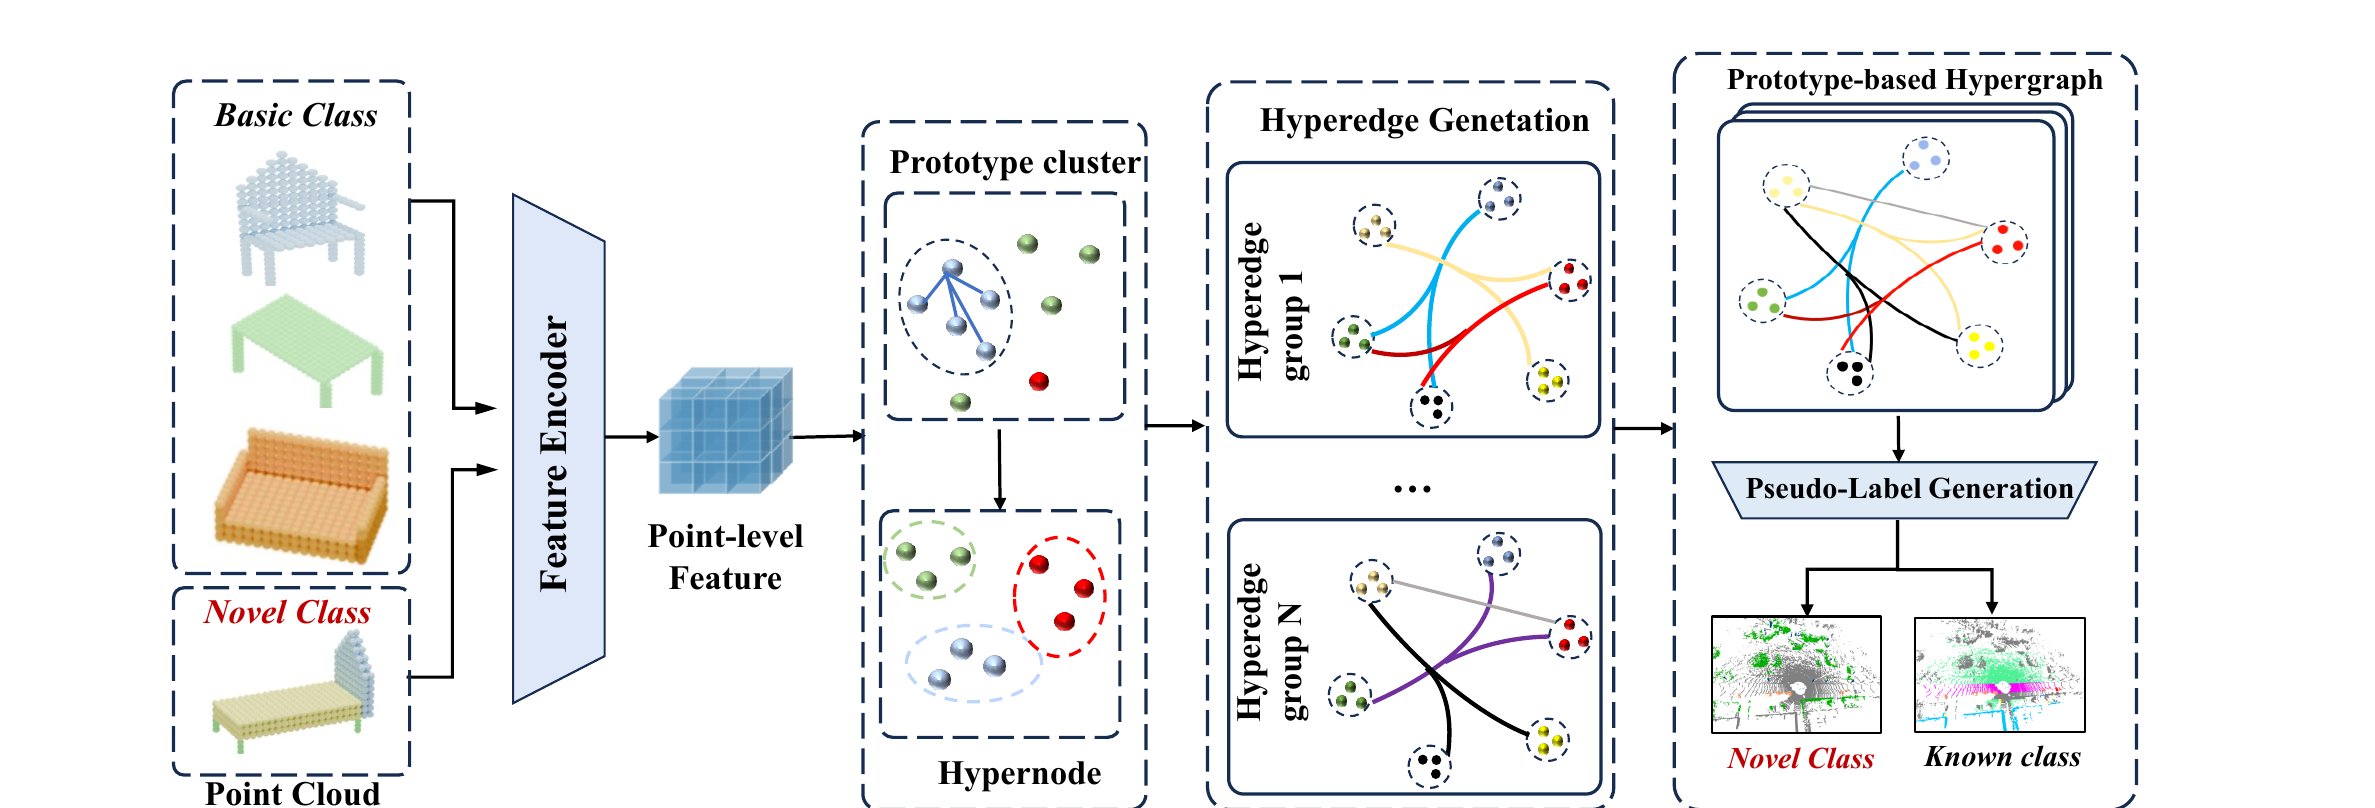
\includegraphics[width=\linewidth]{imagenes/arq_hyperncd_paper.png}
\caption[Arquitectura de HyperNCD]{Arquitectura de HyperNCD. Fuente: Zhang et al.~\cite{zhang2026hyperncd},
Fig.~2.}
\label{fig:arq-hyperncd-paper}
\end{figure}

HyperNCD~\cite{zhang2026hyperncd} resuelve el NCD en cuatro etapas, que la
Figura~\ref{fig:arq-hyperncd-paper} presenta de izquierda a derecha:

\begin{enumerate}\setlength{\itemsep}{2pt}
\item \textbf{Codificador de características} (\emph{Feature Encoder}). La nube,
con puntos de clases conocidas y novedosas mezclados, entra a una red troncal que
asigna a cada punto un vector de características (\emph{point-level feature}).
En la implementación es la MinkowskiUNet-34C que produce $f_{\mathrm{sem}}$.
\item \textbf{Agrupamiento en prototipos} (\emph{Prototype cluster}). Una
convolución unidimensional seguida de \emph{softmax} reparte los puntos entre $K$
prototipos (Sección~\ref{sec:prototipo}); cada prototipo pasa a ser un nodo del
hipergrafo (\emph{hypernode}).
\item \textbf{Generación de hiperaristas} (\emph{Hyperedge generation}). Cada
prototipo se une a sus $M$ más afines según la afinidad $S_b$ de la
Ec.~\eqref{eq:afinidad}, que combina parecido geométrico y semántico. En cada
lote se forma un grupo de hiperaristas.
\item \textbf{Hipergrafo de prototipos y pseudo-etiquetas}
(\emph{Prototype-based hypergraph}). Las hiperaristas se reajustan a medida que
llegan lotes nuevos. Un prototipo cuya afinidad con uno conocido supera un umbral
recibe la etiqueta de esa clase; si no, se considera novedoso y recibe una
etiqueta nueva. Esas pseudo-etiquetas vuelven al entrenamiento.
\end{enumerate}

La figura corresponde a la formulación del artículo. La implementación publicada
que este trabajo ejecuta realiza las tres primeras etapas, pero no el reajuste
dinámico de la cuarta, y asigna las pseudo-etiquetas con Sinkhorn-Knopp en lugar
del umbral (Anexo~D). Además, en la implementación los nodos del hipergrafo son
regiones y no prototipos (Sección~\ref{sec:hiperarista}); este trabajo adopta esa
formulación.

\subsection{Arquitectura de Sonata}
\label{sec:arq-sonata-paper}

\begin{figure}[H]
\centering
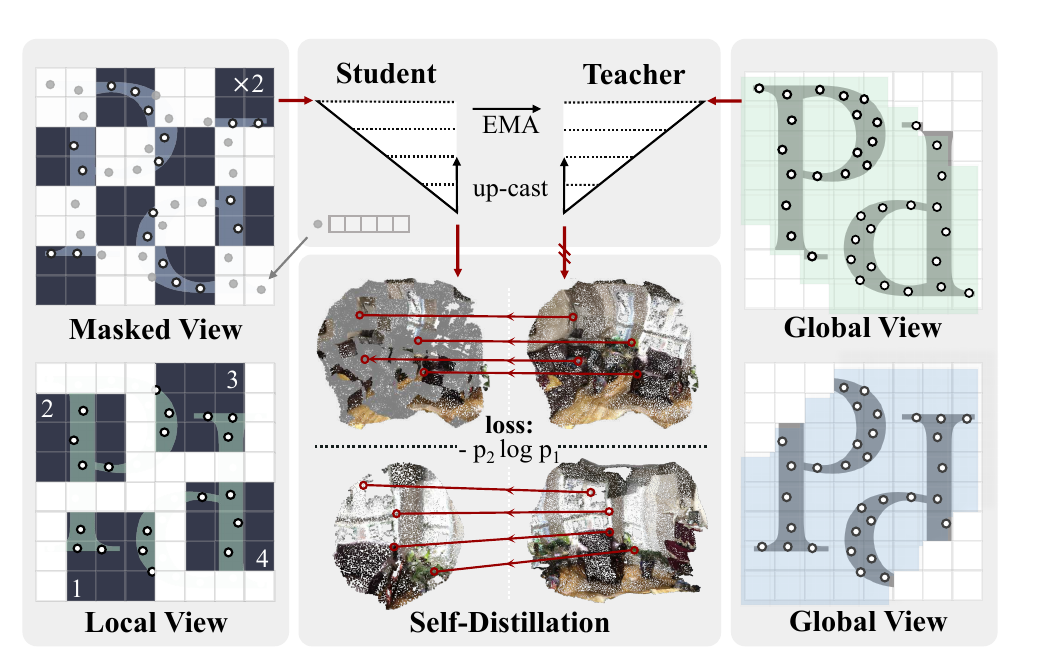
\includegraphics[width=0.82\linewidth]{imagenes/arq_sonata_paper.png}
\caption[Auto-destilación de Sonata]{Marco de auto-destilación de Sonata. Fuente: Wu et
al.~\cite{wu2025sonata}, Fig.~5.}
\label{fig:arq-sonata-paper}
\end{figure}

Sonata~\cite{wu2025sonata} no es un clasificador, sino un método para preentrenar
un codificador sin etiquetas. La Figura~\ref{fig:arq-sonata-paper} muestra cómo se
entrenó; este trabajo usa únicamente el codificador resultante, congelado. El
entrenamiento es una auto-destilación entre dos copias de la misma red:

\begin{itemize}\setlength{\itemsep}{2pt}
\item \textbf{Tres tipos de vista.} De cada escena se generan vistas globales,
amplias y completas (derecha); vistas locales, recortes pequeños (abajo a la
izquierda); y vistas enmascaradas, en las que se ocultan parches de una rejilla
(arriba a la izquierda).
\item \textbf{Estudiante y maestro} (\emph{student}, \emph{teacher}). El
estudiante procesa las vistas locales y enmascaradas; el maestro, las globales.
El maestro no se entrena directamente. Sus pesos son una media móvil
exponencial (EMA) de los del estudiante, lo que lo hace más estable.
\item \textbf{Destilación.} Cada punto de una vista local o enmascarada se
empareja con el punto de la vista global que ocupa la misma posición, y el
estudiante aprende a reproducir lo que el maestro dice de ese punto. La pérdida
$-p_2\log p_1$ es una entropía cruzada que toma la distribución del maestro
($p_2$) como objetivo para la del estudiante ($p_1$). Como el estudiante ve menos
contexto que el maestro, para acertar tiene que aprender qué es el punto y no
solo su geometría local.
\item \textbf{Codificador sin decodificador y \emph{up-cast}.} La red es un PTv3
al que se le quitó el decodificador, porque este favorecía el atajo geométrico
(Sección~\ref{sec:atajo}); para conservar información de varias escalas, las
características se devuelven a la resolución de las etapas anteriores mediante
el \emph{up-cast} (Sección~\ref{sec:upcast}).
\end{itemize}

% =====================================================================
\section{Métricas de Evaluación de Modelos}
\label{sec:metricas}

Para evaluar la efectividad del modelo se utilizan las métricas siguientes.

\subsection{Intersection over Union (IoU)}
\label{sec:iou}

Para una clase $c$, la intersección sobre unión se define como:
\begin{equation}
\mathrm{IoU}_c=\frac{TP_c}{TP_c+FP_c+FN_c},
\label{eq:iou}
\end{equation}
donde $TP_c$, $FP_c$ y $FN_c$ son los puntos verdaderos positivos, falsos
positivos y falsos negativos de esa clase.

\subsection{IoU Media (mIoU)}
\label{sec:miou}

La métrica agregada es el promedio de la anterior sobre un conjunto de clases:
\begin{equation}
\mathrm{mIoU}(\mathcal{S})=\frac{1}{|\mathcal{S}|}\sum_{c\in\mathcal{S}}\mathrm{IoU}_c,
\qquad
\mathcal{S}\in\{\mathcal{C}_k,\;\mathcal{C}_n,\;\mathcal{C}\}.
\label{eq:miou}
\end{equation}
Se reporta por separado como mIoU \emph{known}, mIoU \emph{novel} y mIoU
\emph{all}.

\subsection{Análisis de Dominancia}
\label{sec:dominancia}

La Ec.~\eqref{eq:miou} es una media aritmética no ponderada, por lo que
\begin{equation}
\frac{\partial\,\mathrm{mIoU}}{\partial\,\mathrm{IoU}_c}=\frac{1}{|\mathcal{S}|}
\qquad \forall\, c\in\mathcal{S}.
\label{eq:dominancia}
\end{equation}
Cada clase pesa igual con independencia de su número de puntos. Por ello el
valor agregado se acompaña siempre de la clase dominante:
\begin{equation}
c^{*}=\arg\max_{c\in\mathcal{S}}\bigl|\mathrm{IoU}_c-\mathrm{mIoU}(\mathcal{S})\bigr|.
\label{eq:dominante}
\end{equation}

\subsection{Emparejamiento Húngaro}
\label{sec:hungaro}

Como las clases de $\mathcal{C}_n$ se descubren sin etiqueta, la correspondencia
entre agrupaciones predichas y clases reales se resuelve por asignación óptima:
\begin{equation}
\sigma^{*}=\arg\max_{\sigma\in\mathfrak{S}_{|\mathcal{C}_n|}}
\sum_{c\in\mathcal{C}_n}\mathrm{IoU}\bigl(\hat{y}=\sigma(c),\;y=c\bigr).
\label{eq:hungaro}
\end{equation}

\subsection{Índice de Rand Ajustado (ARI)}
\label{sec:ari}

Mide la coincidencia entre la agrupación descubierta y la real con independencia
del emparejamiento:
\begin{equation}
\mathrm{ARI}=
\frac{\sum_{ij}\binom{n_{ij}}{2}
-\Bigl[\sum_i\binom{a_i}{2}\sum_j\binom{b_j}{2}\Bigr]\big/\binom{n}{2}}
{\tfrac{1}{2}\Bigl[\sum_i\binom{a_i}{2}+\sum_j\binom{b_j}{2}\Bigr]
-\Bigl[\sum_i\binom{a_i}{2}\sum_j\binom{b_j}{2}\Bigr]\big/\binom{n}{2}},
\label{eq:ari}
\end{equation}
donde $n_{ij}$ es el número de puntos comunes entre la agrupación $i$ y la clase
$j$, y $a_i$ y $b_j$ sus marginales.

\subsection{Información Mutua Normalizada (NMI)}
\label{sec:nmi}

Complementa al ARI midiendo la información que una agrupación aporta sobre la
otra:
\begin{equation}
\mathrm{NMI}(U,V)=\frac{2\,I(U;V)}{H(U)+H(V)},
\label{eq:nmi}
\end{equation}
donde $I$ es la información mutua y $H$ la entropía.

\subsection{Linear Probing}
\label{sec:probing}

Protocolo de evaluación de un descriptor congelado, en el que se entrena únicamente un
clasificador lineal $W$ sobre él,
\begin{equation}
\hat{y}_i=\arg\max\left(W^{\top}f_{\mathrm{ssl}}(x^i)+b\right),
\label{eq:probe}
\end{equation}
de modo que el desempeño resultante queda atribuido a la representación y no al
clasificador.

\subsection{Ganancia Absoluta}
\label{sec:ganancia}

Diferencia de mIoU sobre las clases novedosas entre el modelo híbrido y la línea
base:
\begin{equation}
\Delta\mathrm{mIoU}^{\mathrm{novel}}=
\mathrm{mIoU}^{\mathrm{novel}}_{\mathrm{hib}}-\mathrm{mIoU}^{\mathrm{novel}}_{\mathrm{base}}.
\label{eq:delta}
\end{equation}

\subsection{Brecha Cerrada}
\label{sec:brecha}

La ganancia absoluta no es interpretable por sí sola, porque el techo alcanzable
depende de la sección. Esta métrica, propuesta en el presente trabajo, la
normaliza por la brecha que separa a la línea base de su propio desempeño sobre
las clases que sí vio etiquetadas:
\begin{equation}
G=\frac{\mathrm{mIoU}^{\mathrm{novel}}_{\mathrm{hib}}-\mathrm{mIoU}^{\mathrm{novel}}_{\mathrm{base}}}
{\mathrm{mIoU}^{\mathrm{known}}_{\mathrm{base}}-\mathrm{mIoU}^{\mathrm{novel}}_{\mathrm{base}}}.
\label{eq:G}
\end{equation}
$G$ es adimensional. $G=0$ indica que la sustitución no aporta, $G=1$ que las
clases novedosas alcanzan la calidad con que el modelo segmenta las conocidas y
$G<0$ degradación.

\subsection{Atribución por Etapas}
\label{sec:metricas-hibrido}

Como el proceso es separable en dos etapas, la métrica se reporta también en el
punto intermedio y no solo al final, con \emph{linear probing} sobre el descriptor
(Ec.~\eqref{eq:probe}) antes de la formación de prototipos y mIoU
(Ec.~\eqref{eq:miou}) después. Esa separación permite atribuir una mejora a la
representación o al razonamiento, y no al sistema tratado como caja negra.

% =====================================================================
\section{Diseño de la Tesis}
\label{sec:diseno-teorico}

La Figura~\ref{fig:diseno} organiza el sistema en cinco módulos, de izquierda a
derecha; sobre cada flecha se indica lo que pasa de un módulo al siguiente. Cada
paso remite al concepto que lo define en las secciones anteriores.

\begin{landscape}
\begin{figure}[H]
\centering
{\hypersetup{linkcolor=blue!55!black}\fuentediagrama
\adjustbox{max width=\linewidth, max totalheight=12.9cm}{% Diagrama de diseno: cinco modulos; el Modulo 4 contiene sus cuatro operaciones.
% Cada linea y cada formula enlaza con el marco teorico (correspondencia uno a uno).
% La incluyen la tesis (capitulo2.tex) y diagrama_diseno.tex (PDF/PNG).
\definecolor{cEnt}{RGB}{31,78,121}
\definecolor{cSem}{RGB}{31,110,60}
\definecolor{cEnc}{RGB}{101,60,140}
\definecolor{cFus}{RGB}{176,32,42}
\definecolor{cSal}{RGB}{191,110,20}
\pgfdeclarelayer{background}
\pgfsetlayers{background,main}
\begin{tikzpicture}[
  font=\scriptsize,
  execute at begin node={\hyphenpenalty=10000\exhyphenpenalty=10000},
  mod/.style={rounded corners=3pt, draw, thick, align=center, inner sep=5pt},
  tab/.style={rounded corners=2pt, text=white, font=\scriptsize\bfseries, inner sep=3pt, anchor=center},
  tarj/.style={rounded corners=2.5pt, draw=black!40, fill=white, semithick,
               align=left, inner sep=4pt, text width=4.3cm, minimum height=3.4cm, anchor=north},
  chico/.style={font=\tiny, text=black!65},
  fl/.style={-{Latex[length=2.1mm]}, thick, black!65}
]
%% ---------- semantica y encoder ----------
\node[mod, draw=cSem, fill=cSem!6, text width=3.9cm, anchor=south] (M2) at (6.25,0.25)
 {{\rule{0pt}{8pt}\scriptsize\bfseries\itshape \hyperref[sec:arq-hyperncd-paper]{\textcolor{cSem}{HyperNCD}}}\\[4pt]
  \tikz[baseline=0, every node/.style={anchor=center, align=center, text width={}, minimum height=0pt, minimum width=0pt, inner sep=1pt}]{
    \foreach \i/\h in {0/0.95, 1/0.72, 2/0.50, 3/0.32}
      \fill[cSem!35, draw=cSem] (\i*0.24,0.5-\h/2) rectangle (\i*0.24+0.16,0.5+\h/2);
    \foreach \i/\h in {0/0.32, 1/0.50, 2/0.72, 3/0.95}
      \fill[cSem!65, draw=cSem] (1.1+\i*0.24,0.5-\h/2) rectangle (1.1+\i*0.24+0.16,0.5+\h/2);
    \foreach \a/\b/\h in {0/3/0.95, 1/2/0.72, 2/1/0.50}
      \draw[cSem!80, densely dashed, -{Latex[length=1mm]}] (\a*0.24+0.16,0.5+\h/2+0.05) -- (1.1+\b*0.24,0.5+\h/2+0.05);
    \draw[-{Latex[length=1.2mm]}, cSem!80, semithick] (0.88,0.5) -- (1.08,0.5);}\\[5pt]
  \begin{minipage}{\linewidth}\raggedright\scriptsize
  \textbf{1.} \hyperref[sec:rejilla]{Indexa en rejilla dispersa}\\
  \textbf{2.} \hyperref[sec:fsem]{Red MinkowskiUNet-34C}~\logo{pytorch.png}\\
  \textbf{3.} \hyperref[sec:clases]{Entrena con clases conocidas}\\
  \textbf{4.} \hyperref[sec:fsem]{Se reentrena cada época}\end{minipage}\\[3pt]
  \hyperref[sec:fsem]{\textbf{$\rightarrow f_{\mathrm{sem}}(x^i)$: 96 números}}};

\node[mod, draw=cEnc, fill=cEnc!6, text width=3.9cm, anchor=north] (M3) at (6.25,-0.25)
 {{\rule{0pt}{8pt}\scriptsize\bfseries\itshape \hyperref[sec:arq-sonata-paper]{\textcolor{cEnc}{Sonata}}}\\[4pt]
  \tikz[baseline=0, every node/.style={anchor=center, align=center, text width={}, minimum height=0pt, minimum width=0pt, inner sep=1pt}]{
    \foreach \i/\w in {0/1.15, 1/0.97, 2/0.79, 3/0.61, 4/0.43}
      \fill[rounded corners=1pt, cEnc!45, draw=cEnc] (0,\i*0.19) rectangle (\w,\i*0.19+0.13);
    \begin{scope}[shift={(1.55,0.5)}]
      \foreach \a in {0,60,120}{
        \draw[cyan!65!black, thick] ({\a}:-0.26) -- ({\a}:0.26);
        \foreach \s in {1,-1}{ \draw[cyan!65!black, semithick] ({\a}:0.17*\s) -- ++({\a+40*\s}:0.08); \draw[cyan!65!black, semithick] ({\a}:0.17*\s) -- ++({\a-40*\s}:0.08);}}
    \end{scope}}\\[5pt]
  \begin{minipage}{\linewidth}\raggedright\scriptsize
  \textbf{1.} \hyperref[sec:serializacion]{Ordena por serialización}\\
  \textbf{2.} \hyperref[sec:ssl]{PTv3 auto-supervisado}\\
  \textbf{3.} \hyperref[sec:atajo]{Sin decoder: sin atajo geom.}\\
  \textbf{4.} \hyperref[sec:congelado]{Congelado: 1 vez, a disco}~\logo{numpy.png}\\
  \textbf{5.} \hyperref[sec:upcast]{\emph{Up-cast} a resolución original}\\
  \textbf{6.} \hyperref[sec:probing]{Calidad: \emph{linear probing}}\end{minipage}\\[3pt]
  \hyperref[sec:fssl]{\textbf{$\rightarrow f_{\mathrm{ssl}}(x^i)$: 1088 números}}\\[1pt]
  {\tiny\hyperref[sec:congelado]{costo: 108\,M parámetros · 4{,}2\,GB de memoria GPU}}};

%% ---------- preprocesamiento ----------
\node[mod, draw=cEnt, fill=cEnt!6, text width=4.3cm, anchor=center] (M1) at (0.0,0)
 {{\rule{0pt}{8pt}\scriptsize\bfseries\itshape \hyperref[sec:tls]{\textcolor{cEnt}{levantamiento TLS}} · \hyperref[sec:modulo1]{\textcolor{cEnt}{hasta 1\,TB}}}\\[4pt]
  \tikz[baseline=0, every node/.style={anchor=center, align=center, text width={}, minimum height=0pt, minimum width=0pt, inner sep=1pt}]{
    \draw[black!35] (0.34,0.23) rectangle (1.59,1.28);
    \draw[black!35] (0,0) -- (0.34,0.23) (1.25,0) -- (1.59,0.23) (1.25,1.05) -- (1.59,1.28) (0,1.05) -- (0.34,1.28);
    \foreach \x/\y/\t in {0.097/0.087/95, 0.089/0.121/98, 0.080/0.175/97, 0.104/0.235/93, 0.139/0.278/89, 0.129/0.332/87, 0.129/0.372/89, 0.106/0.408/92, 0.135/0.448/87, 0.142/0.512/86, 0.117/0.540/93, 0.159/0.598/85, 0.104/0.595/97, 0.101/0.671/94, 0.121/0.703/92, 0.118/0.750/91, 0.132/0.815/89, 0.168/0.875/84, 0.148/0.892/86, 0.139/0.944/90, 0.148/0.980/87, 0.087/0.988/98, 0.163/0.103/93, 0.165/0.134/93, 0.198/0.218/83, 0.129/0.216/96, 0.215/0.297/82, 0.233/0.353/79, 0.179/0.362/87, 0.155/0.397/91, 0.150/0.427/95, 0.226/0.521/80, 0.191/0.543/88, 0.187/0.597/87, 0.213/0.657/81, 0.195/0.685/85, 0.204/0.736/81, 0.145/0.742/95, 0.141/0.786/95, 0.152/0.835/94, 0.197/0.904/85, 0.191/0.955/85, 0.174/0.976/87, 0.193/1.022/88, 0.235/0.109/86, 0.242/0.163/83, 0.254/0.215/81, 0.241/0.260/82, 0.257/0.300/80, 0.227/0.325/86, 0.236/0.364/86, 0.231/0.430/85, 0.243/0.456/86, 0.244/0.522/85, 0.234/0.547/84, 0.255/0.623/80, 0.252/0.651/80, 0.236/0.690/86, 0.249/0.738/81, 0.227/0.767/86, 0.269/0.837/78, 0.261/0.870/78, 0.251/0.920/84, 0.239/0.953/87, 0.263/1.014/81, 0.231/1.026/86, 0.300/0.122/80, 0.263/0.160/88, 0.349/0.247/73, 0.323/0.279/78, 0.262/0.294/86, 0.298/0.354/81, 0.308/0.410/79, 0.324/0.447/75, 0.292/0.482/83, 0.315/0.539/76, 0.322/0.595/75, 0.279/0.600/87, 0.276/0.645/87, 0.297/0.694/81, 0.320/0.756/76, 0.258/0.755/87, 0.324/0.841/74, 0.317/0.867/80, 0.286/0.906/83, 0.299/0.960/82, 0.265/0.982/87, 0.297/1.051/82, 0.340/0.125/80, 0.359/0.188/79, 0.369/0.231/78, 0.374/0.282/74, 0.358/0.320/78, 0.369/0.370/75, 0.343/0.396/79, 0.368/0.456/78, 0.361/0.491/80, 0.385/0.541/72, 0.390/0.605/72, 0.374/0.634/76, 0.314/0.644/85, 0.318/0.694/85, 0.376/0.760/72, 0.377/0.801/73, 0.363/0.858/75, 0.381/0.904/75, 0.394/0.933/72, 0.336/0.961/83, 0.341/1.010/83, 0.381/1.078/72, 0.395/0.130/78, 0.418/0.197/75, 0.407/0.228/77, 0.419/0.271/74, 0.456/0.339/70, 0.429/0.386/71, 0.427/0.415/74, 0.402/0.452/79, 0.438/0.526/69, 0.438/0.555/71, 0.390/0.567/79, 0.406/0.616/78, 0.414/0.680/77, 0.455/0.737/68, 0.405/0.745/78, 0.397/0.800/77, 0.398/0.838/77, 0.467/0.912/66, 0.419/0.941/75, 0.438/0.997/73, 0.447/1.050/69, 0.452/1.099/67, 0.458/0.140/76, 0.518/0.231/64, 0.468/0.227/76, 0.485/0.291/69, 0.472/0.335/75, 0.485/0.372/72, 0.457/0.393/77, 0.479/0.455/73, 0.445/0.491/79, 0.472/0.551/72, 0.501/0.620/65, 0.447/0.624/77, 0.443/0.670/78, 0.462/0.722/77, 0.512/0.785/67, 0.499/0.821/69, 0.467/0.858/75, 0.499/0.926/69, 0.479/0.938/72, 0.486/1.006/69, 0.491/1.035/69, 0.511/1.090/65, 0.568/0.177/63, 0.537/0.215/67, 0.546/0.262/67, 0.507/0.277/74, 0.537/0.358/66, 0.523/0.385/72, 0.551/0.443/64, 0.499/0.459/74, 0.528/0.506/72, 0.549/0.574/66, 0.499/0.594/75, 0.497/0.618/76, 0.518/0.683/74, 0.540/0.744/66, 0.549/0.791/68, 0.499/0.805/74, 0.511/0.855/74, 0.490/0.895/77, 0.574/0.987/62, 0.534/1.003/68, 0.550/1.064/67, 0.525/1.094/70, 0.550/0.153/75, 0.590/0.219/68, 0.562/0.243/73, 0.584/0.290/68, 0.592/0.348/67, 0.570/0.383/73, 0.559/0.416/75, 0.548/0.450/74, 0.571/0.524/71, 0.568/0.553/73, 0.624/0.633/61, 0.578/0.652/70, 0.618/0.726/62, 0.580/0.746/68, 0.541/0.751/75, 0.574/0.818/68, 0.583/0.869/69, 0.585/0.909/68, 0.568/0.942/73, 0.585/1.003/70, 0.586/1.052/67, 0.554/1.063/73, 0.607/0.721/73, 0.602/0.781/71, 0.670/0.851/61, 0.609/0.856/71, 0.629/0.914/69, 0.653/0.989/60, 0.600/0.970/74, 0.586/1.018/74, 0.647/1.116/61, 0.652/0.765/72, 0.697/0.844/64, 0.648/0.858/72, 0.679/0.905/68, 0.654/0.948/73, 0.679/1.022/65, 0.682/1.057/68, 0.674/1.092/70, 0.757/0.840/62, 0.688/0.860/71, 0.736/0.927/65, 0.692/0.985/73, 0.749/1.066/63, 0.708/1.092/68, 0.799/0.847/61, 0.797/0.884/62, 0.766/0.915/65, 0.719/0.937/75, 0.751/0.988/71, 0.747/1.041/72, 0.741/1.081/70, 0.813/0.847/66, 0.780/0.836/75, 0.783/0.986/71, 0.783/1.026/71, 0.825/1.108/64, 0.822/0.776/73, 0.822/0.794/76, 0.852/0.872/67, 0.840/0.917/71, 0.816/0.949/72, 0.851/1.015/66, 0.809/1.033/74, 0.860/1.109/66, 0.848/0.757/75, 0.820/0.786/81, 0.827/0.845/80, 0.900/0.906/68, 0.834/0.922/81, 0.826/0.974/79, 0.878/1.052/69, 0.851/1.084/74, 0.881/0.706/79, 0.865/0.745/83, 0.913/0.823/73, 0.905/0.869/73, 0.859/0.864/82, 0.872/0.938/79, 0.857/0.934/86, 0.927/1.043/72, 0.908/1.070/75, 0.902/0.128/82, 0.895/0.167/84, 0.900/0.202/85, 0.945/0.285/74, 0.944/0.325/78, 0.893/0.349/85, 0.924/0.403/77, 0.895/0.428/85, 0.919/0.472/83, 0.949/0.554/75, 0.922/0.569/80, 0.931/0.626/76, 0.943/0.656/77, 0.902/0.703/84, 0.936/0.762/75, 0.927/0.804/78, 0.911/0.824/81, 0.922/0.876/79, 0.894/0.898/88, 0.917/0.963/79, 0.894/0.986/84, 0.912/1.038/81, 0.963/0.124/83, 0.974/0.185/80, 0.911/0.189/91, 0.943/0.239/87, 0.923/0.267/91, 0.914/0.314/93, 0.896/0.353/92, 0.928/0.400/90, 0.932/0.463/86, 0.936/0.509/87, 0.947/0.578/82, 0.951/0.610/81, 0.911/0.602/94, 0.967/0.701/80, 0.938/0.717/88, 0.919/0.767/90, 0.948/0.812/83, 0.933/0.876/84, 0.921/0.879/90, 0.941/0.959/85, 0.947/1.013/83, 0.925/1.017/89, 0.972/0.091/90, 0.985/0.154/86, 0.987/0.207/87, 0.955/0.221/90, 0.988/0.289/83, 0.991/0.353/82, 0.951/0.374/90, 0.927/0.381/96, 0.989/0.466/84, 0.962/0.477/92, 0.945/0.521/93, 0.949/0.583/91, 0.954/0.621/89, 0.980/0.674/87, 0.968/0.727/87, 0.952/0.763/90, 0.974/0.811/88, 0.984/0.849/85, 0.975/0.891/89, 0.974/0.956/86, 0.995/1.012/82, 0.961/1.036/89, 0.973/0.090/95, 0.964/0.115/100, 0.988/0.185/94, 0.986/0.227/94, 1.012/0.282/89, 1.003/0.313/89, 1.018/0.365/88, 1.030/0.418/87, 0.979/0.434/97, 0.999/0.503/89, 0.992/0.531/92, 0.990/0.581/92, 0.991/0.608/92, 0.963/0.650/98, 0.981/0.691/95, 0.958/0.714/100, 0.989/0.783/93, 0.987/0.828/92, 0.996/0.885/94, 0.971/0.900/97, 0.959/0.960/99, 0.991/1.002/96, 0.988/0.076/100, 0.993/0.106/100, 1.031/0.193/92, 0.989/0.198/100, 0.997/0.244/100, 1.001/0.300/100, 1.030/0.337/96, 1.001/0.379/99, 1.020/0.431/98, 1.039/0.482/93, 1.016/0.522/96, 0.989/0.532/100, 1.035/0.606/94, 1.039/0.675/92, 0.985/0.663/100, 1.045/0.760/91, 1.044/0.794/90, 1.035/0.831/94, 1.021/0.877/94, 0.989/0.882/100, 0.990/0.945/100, 1.027/1.003/92, 1.074/0.088/94, 1.056/0.111/98, 1.046/0.159/97, 1.036/0.187/100, 1.008/0.234/100, 1.066/0.293/97, 1.026/0.324/100, 1.057/0.386/96, 1.031/0.405/100, 1.039/0.460/99, 1.025/0.495/100, 1.021/0.530/100, 1.018/0.583/100, 1.055/0.643/99, 1.038/0.673/100, 1.058/0.726/96, 1.070/0.775/95, 1.037/0.809/100, 1.010/0.853/100, 1.010/0.893/100, 1.021/0.928/100, 1.011/0.956/100, 1.081/0.050/100, 1.040/0.083/100, 1.067/0.133/100, 1.037/0.163/100, 1.102/0.239/98, 1.037/0.272/100, 1.062/0.327/100, 1.080/0.364/100, 1.061/0.411/100, 1.043/0.411/100, 1.064/0.497/100, 1.062/0.530/100, 1.032/0.559/100, 1.046/0.618/100, 1.056/0.653/100, 1.102/0.737/98, 1.054/0.738/100, 1.065/0.798/100, 1.045/0.819/100, 1.060/0.880/100, 1.067/0.944/100, 1.031/0.950/100, 1.089/0.041/100, 1.079/0.066/100, 1.098/0.129/100, 1.069/0.160/100, 1.091/0.210/100, 1.073/0.245/100, 1.108/0.320/100, 1.130/0.358/100, 1.135/0.420/100, 1.117/0.465/100, 1.120/0.507/100, 1.120/0.555/100, 1.073/0.546/100, 1.087/0.599/100, 1.076/0.656/100, 1.073/0.706/100, 1.077/0.746/100, 1.069/0.788/100, 1.070/0.831/100, 1.088/0.859/100, 1.094/0.924/100, 1.079/0.954/100, 1.150/0.055/100, 1.113/0.052/100, 1.153/0.136/100, 1.137/0.177/100, 1.086/0.187/100, 1.118/0.234/100, 1.164/0.307/100, 1.093/0.327/100, 1.122/0.372/100, 1.110/0.417/100, 1.084/0.453/100, 1.108/0.494/100, 1.109/0.541/100, 1.114/0.592/100, 1.141/0.661/100, 1.123/0.697/100, 1.143/0.744/100, 1.126/0.776/100, 1.122/0.810/100, 1.126/0.856/100, 1.121/0.907/100, 1.102/0.944/100} \fill[cEnt!\t] (\x,\y) circle (0.013);
    \draw[black!55, semithick] (0,0) rectangle (1.25,1.05);}\\[5pt]
  \begin{minipage}{\linewidth}\raggedright\scriptsize
  \textbf{1.} \hyperref[sec:las]{Lectura por bloques del .LAS}\\
  \textbf{2.} \hyperref[sec:seccion]{Corte en 5 secciones $S_j$}~\logo{numpy.png}\\
  \textbf{3.} \hyperref[sec:sor]{Limpieza de ruido (SOR)}~\logo{open3d.png}\\
  \textbf{4.} \hyperref[sec:voxel]{Voxelización a 5\,cm}~\logo{open3d.png}\\
  \textbf{5.} \hyperref[sec:normales]{Normales por vecindad}~\logo{open3d.png}\end{minipage}};

%% ---------- fusion ----------
\node[align=center, anchor=north, text width=9cm] (M4h) at (15.8,4.4)
 {{\rule{0pt}{8pt}\scriptsize\bfseries\itshape \hyperref[sec:arq-hyperncd-paper]{\textcolor{cFus}{HyperNCD}} · \hyperref[sec:ncd]{\textcolor{cFus}{descubre clases novedosas}}}};

\node[tarj] (T1) at ($(M4h.south)+(-3.0,-0.3)$)
 {\enlace{sec:concat}{\textbf{\textcircled{\scriptsize 1} Concatenación}}\\[3pt]
  \centering
  \tikz[baseline=0, every node/.style={anchor=center, align=center, text width={}, minimum height=0pt, minimum width=0pt, inner sep=1pt}]{
    \fill[cSem!45, draw=cSem] (0,0) rectangle (0.36,0.22);
    \fill[cEnc!45, draw=cEnc] (0.36,0) rectangle (2.2,0.22);
    \node[font=\tiny] at (0.18,0.11) {\hyperref[sec:fsem]{96}};
    \node[font=\tiny] at (1.28,0.11) {\hyperref[sec:fssl]{1088}};
    \fill[cSem!45, draw=cSem] (2.45,0) rectangle (2.81,0.22);
    \fill[red!30, draw=cFus] (2.81,0) rectangle (2.93,0.22);
    \node[font=\tiny, text=black!60] at (2.69,-0.16) {\hyperref[sec:fgeo]{antes}};}\\[5pt]
  \centering \enlaceec{eq:hibrido}{$F_i=\left[\,f_{\mathrm{sem}};\,f_{\mathrm{ssl}}\,\right]$}\\[5pt]
  \raggedright
  \textbf{1.} \hyperref[sec:fsem]{$f_{\mathrm{sem}}$: 96 valores semánticos}\\
  \textbf{2.} \hyperref[sec:fssl]{$f_{\mathrm{ssl}}$: 1088, auto-supervisado}\\
  \textbf{3.} \hyperref[sec:descriptor]{Descriptor $F_i$: 1184 valores}\\
  \textbf{4.} \hyperref[sec:fgeo]{Sustituye a $f_{\mathrm{geo}}$ (6, manual)}};

\node[tarj] (T2) at ($(M4h.south)+(3.0,-0.3)$)
 {\enlace{sec:formproto}{\textbf{\textcircled{\scriptsize 2} Prototipos}}~\logo{pytorch.png}\\[3pt]
  \centering
  \tikz[baseline=0, every node/.style={anchor=center, align=center, text width={}, minimum height=0pt, minimum width=0pt, inner sep=1pt}]{\begin{scope}[scale=0.85]
    \foreach \x/\y/\c in {0.222/0.339/cSem, 0.457/0.245/cSem, 0.212/0.293/cSem, 0.401/0.416/cSem, 0.234/0.177/cSem, 0.429/0.353/cSem, 0.494/0.392/cSem, 0.330/0.247/cSem, 1.343/0.558/cEnc, 1.069/0.463/cEnc, 1.179/0.624/cEnc, 1.092/0.570/cEnc, 1.182/0.660/cEnc, 1.267/0.602/cEnc, 0.986/0.644/cEnc, 1.005/0.562/cEnc, 1.651/0.120/cSal, 1.712/0.144/cSal, 1.999/0.117/cSal, 1.884/-0.012/cSal, 1.766/0.197/cSal, 1.785/0.179/cSal, 1.811/0.011/cSal, 1.862/0.031/cSal} \fill[\c!55] (\x,\y) circle (0.035);
    \foreach \x/\y/\c in {0.35/0.30/cSem, 1.15/0.58/cEnc, 1.80/0.12/cSal}
      \node[star, star points=5, star point ratio=2.2, draw=\c, fill=\c!35, inner sep=0.6pt] at (\x,\y) {};
    \fill[black] (0.80,0.20) circle (0.042);
    \draw[dashed, black!55] (0.80,0.20) -- (0.35,0.30);
    \draw[dashed, black!55] (0.80,0.20) -- (1.15,0.58);
    \node[font=\tiny, text=black!60] at (0.52,0.02) {\hyperref[sec:formproto]{70\,\%}};
    \node[font=\tiny, text=black!60] at (1.22,0.20) {\hyperref[sec:formproto]{30\,\%}};\end{scope}}\\[5pt]
  \centering \enlaceec{eq:softmax}{$s_{i,k}=\frac{e^{z_{i,k}}}{\sum_{j}e^{z_{i,j}}}$}\\[5pt]
  \raggedright
  \textbf{1.} \hyperref[sec:formproto]{Puntuación $z_{i,k}$ por grupo}\\
  \textbf{2.} \hyperref[sec:formproto]{\emph{Softmax}: reparto $s_{i,k}$, suma 1}\\
  \textbf{3.} \hyperref[sec:prototipo]{Prototipo $P_k$: media ponderada}\\
  \textbf{4.} \hyperref[sec:formproto]{$K$ = número de clases}};

\node[tarj] (T3) at ($(T2.south)+(0,-0.8)$)
 {\enlace{sec:afinhiper}{\textbf{\textcircled{\scriptsize 3} Afinidad e hiperaristas}}\\[3pt]
  \centering
  \tikz[baseline=0, every node/.style={anchor=center, align=center, text width={}, minimum height=0pt, minimum width=0pt, inner sep=1pt}]{\begin{scope}[scale=0.85]
    \fill[cSem!25, draw=cSem!60, rotate=20] (0.72,0.26) ellipse (0.80 and 0.34);
    \fill[cEnc!25, draw=cEnc!60, rotate=-15] (1.42,0.52) ellipse (0.74 and 0.32);
    \foreach \x/\y in {0.25/0.20, 0.72/0.46, 1.05/0.14, 1.55/0.40, 1.98/0.12, 1.62/0.70}
      \fill[black!75] (\x,\y) circle (0.05);\end{scope}}\\[5pt]
  \centering \enlaceec{eq:afinidad}{$S_b=\alpha S_g+(1-\alpha)S_s$}\\[5pt]
  \raggedright
  \textbf{1.} \hyperref[eq:gauss]{$S_g$: forma de la región, $\tau=0{,}1$}\\
  \textbf{2.} \hyperref[eq:coseno]{$S_s$: parecido de significado}\\
  \textbf{3.} \hyperref[sec:afinidad]{$\alpha$: peso forma vs. significado}\\
  \textbf{4.} \hyperref[sec:hiperarista]{Hiperarista: $M=8$ regiones}};

\node[tarj] (T4) at ($(T1.south)+(0,-0.8)$)
 {\enlace{sec:pseudoetq}{\textbf{\textcircled{\scriptsize 4} Pseudo-etiquetas}}\\[3pt]
  \centering
  \tikz[baseline=0, every node/.style={anchor=center, align=center, text width={}, minimum height=0pt, minimum width=0pt, inner sep=1pt}]{
    \foreach \i/\h/\c in {0/0.62/cSem, 1/0.16/cEnc, 2/0.08/cSal}
      \fill[\c!55, draw=\c] (\i*0.26,0) rectangle (\i*0.26+0.2,\h);
    \draw[-{Latex[length=1.3mm]}, black!55] (0.95,0.28) -- (1.4,0.28);
    \foreach \i/\c in {0/cSem, 1/cEnc, 2/cSal}
      \fill[\c!55, draw=\c] (1.6+\i*0.26,0) rectangle (1.6+\i*0.26+0.2,0.28);}\\[5pt]
  \raggedright
  \textbf{1.} \hyperref[sec:pseudo]{Pseudo-etiqueta por grupo}\\
  \textbf{2.} \hyperref[sec:sinkhorn]{Sinkhorn-Knopp: equilibra}\\
  \textbf{3.} \hyperref[sec:pseudoetq]{Suavizado $\epsilon=0{,}15$}\\
  \textbf{4.} \hyperref[sec:pseudoetq]{Vuelven al entrenamiento}};

\begin{pgfonlayer}{background}
\node[fit=(M4h)(T1)(T2)(T3)(T4), draw=cFus, very thick, fill=cFus!5,
      rounded corners=3pt, inner sep=7pt] (M4) {};
\end{pgfonlayer}
\draw[fl] (T1.east |- T2.west) -- (T2.west)
  node[midway, above=0.3mm, chico, fill=cFus!5, inner sep=1pt, align=center]
  {\hyperref[eq:hibrido]{$F_i$}\\por \hyperref[sec:region]{región}};
\draw[fl] (T2.south) -- (T3.north)
  node[midway, right=0.4mm, chico, fill=cFus!5, inner sep=1pt] {\hyperref[sec:region]{regiones} y \hyperref[eq:prototipo]{$P_k$}};
\draw[fl] (T3.west |- T4.east) -- (T4.east)
  node[midway, above=0.3mm, chico, fill=cFus!5, inner sep=1pt, align=center]
  {\hyperref[sec:hipergrafo]{hipergrafo}\\\hyperref[sec:hipergrafo]{$\mathcal{H}$}};

%% ---------- salida ----------
\node[mod, draw=cSal, fill=cSal!6, text width=4.6cm, anchor=west] (M5) at ($(M4.east)+(1.35,0)$)
 {{\rule{0pt}{8pt}\scriptsize\bfseries\itshape \hyperref[sec:modulo5]{\textcolor{cSal}{evaluación y plataforma}}}\\[4pt]
  \tikz[baseline=0, every node/.style={anchor=center, align=center, text width={}, minimum height=0pt, minimum width=0pt, inner sep=1pt}]{
    \draw[black!35] (0.34,0.23) rectangle (1.59,1.28);
    \draw[black!35] (0,0) -- (0.34,0.23) (1.25,0) -- (1.59,0.23) (1.25,1.05) -- (1.59,1.28) (0,1.05) -- (0.34,1.28);
    \foreach \x/\y/\c in {0.097/0.087/cSal, 0.089/0.121/cSal, 0.080/0.175/cSem, 0.104/0.235/cSem, 0.139/0.278/cSem, 0.129/0.332/cSem, 0.129/0.372/cSem, 0.106/0.408/cSem, 0.135/0.448/cSem, 0.142/0.512/cSem, 0.117/0.540/cSem, 0.159/0.598/cSem, 0.104/0.595/cSem, 0.101/0.671/cSem, 0.121/0.703/cSem, 0.118/0.750/cSem, 0.132/0.815/cSem, 0.168/0.875/cSem, 0.148/0.892/cSem, 0.139/0.944/cSem, 0.148/0.980/cSem, 0.087/0.988/cSem, 0.163/0.103/cSal, 0.165/0.134/cSal, 0.198/0.218/cSem, 0.129/0.216/cSem, 0.215/0.297/cSem, 0.233/0.353/cSem, 0.179/0.362/cSem, 0.155/0.397/cSem, 0.150/0.427/cSem, 0.226/0.521/cSem, 0.191/0.543/cSem, 0.187/0.597/cSem, 0.213/0.657/cSem, 0.195/0.685/cSem, 0.204/0.736/cSem, 0.145/0.742/cSem, 0.141/0.786/cSem, 0.152/0.835/cSem, 0.197/0.904/cSem, 0.191/0.955/cSem, 0.174/0.976/cSem, 0.193/1.022/cSem, 0.235/0.109/cSal, 0.242/0.163/cSal, 0.254/0.215/cSem, 0.241/0.260/cSem, 0.257/0.300/cSem, 0.227/0.325/cSem, 0.236/0.364/cSem, 0.231/0.430/cSem, 0.243/0.456/cSem, 0.244/0.522/cSem, 0.234/0.547/cSem, 0.255/0.623/cSem, 0.252/0.651/cSem, 0.236/0.690/cSem, 0.249/0.738/cSem, 0.227/0.767/cSem, 0.269/0.837/cSem, 0.261/0.870/cSem, 0.251/0.920/cSem, 0.239/0.953/cSem, 0.263/1.014/cSem, 0.231/1.026/cSem, 0.300/0.122/cSal, 0.263/0.160/cSal, 0.349/0.247/cSem, 0.323/0.279/cSem, 0.262/0.294/cSem, 0.298/0.354/cSem, 0.308/0.410/cSem, 0.324/0.447/cSem, 0.292/0.482/cSem, 0.315/0.539/cSem, 0.322/0.595/cSem, 0.279/0.600/cSem, 0.276/0.645/cSem, 0.297/0.694/cSem, 0.320/0.756/cSem, 0.258/0.755/cSem, 0.324/0.841/cSem, 0.317/0.867/cSem, 0.286/0.906/cSem, 0.299/0.960/cSem, 0.265/0.982/cSem, 0.297/1.051/cSem, 0.340/0.125/cSal, 0.359/0.188/cSal, 0.369/0.231/cSem, 0.374/0.282/cSem, 0.358/0.320/cSem, 0.369/0.370/cSem, 0.343/0.396/cSem, 0.368/0.456/cSem, 0.361/0.491/cSem, 0.385/0.541/cSem, 0.390/0.605/cSem, 0.374/0.634/cSem, 0.314/0.644/cSem, 0.318/0.694/cSem, 0.376/0.760/cSem, 0.377/0.801/cSem, 0.363/0.858/cSem, 0.381/0.904/cSem, 0.394/0.933/cSem, 0.336/0.961/cSem, 0.341/1.010/cSem, 0.381/1.078/cSem, 0.395/0.130/cSal, 0.418/0.197/cSal, 0.407/0.228/cSem, 0.419/0.271/cSem, 0.456/0.339/cSem, 0.429/0.386/cSem, 0.427/0.415/cSem, 0.402/0.452/cSem, 0.438/0.526/cSem, 0.438/0.555/cSem, 0.390/0.567/cSem, 0.406/0.616/cSem, 0.414/0.680/cSem, 0.455/0.737/cSem, 0.405/0.745/cSem, 0.397/0.800/cSem, 0.398/0.838/cSem, 0.467/0.912/cSem, 0.419/0.941/cSem, 0.438/0.997/cSem, 0.447/1.050/cSem, 0.452/1.099/cSem, 0.458/0.140/cSal, 0.518/0.231/cSal, 0.468/0.227/cSal, 0.485/0.291/cEnc, 0.472/0.335/cEnc, 0.485/0.372/cEnc, 0.457/0.393/cEnc, 0.479/0.455/cEnc, 0.445/0.491/cEnc, 0.472/0.551/cEnc, 0.501/0.620/cEnc, 0.447/0.624/cEnc, 0.443/0.670/cEnc, 0.462/0.722/cEnc, 0.512/0.785/cEnc, 0.499/0.821/cEnc, 0.467/0.858/cEnc, 0.499/0.926/cEnc, 0.479/0.938/cEnc, 0.486/1.006/cEnc, 0.491/1.035/cEnc, 0.511/1.090/cEnc, 0.568/0.177/cSal, 0.537/0.215/cSal, 0.546/0.262/cEnc, 0.507/0.277/cEnc, 0.537/0.358/cEnc, 0.523/0.385/cEnc, 0.551/0.443/cEnc, 0.499/0.459/cEnc, 0.528/0.506/cEnc, 0.549/0.574/cEnc, 0.499/0.594/cEnc, 0.497/0.618/cEnc, 0.518/0.683/cEnc, 0.540/0.744/cEnc, 0.549/0.791/cEnc, 0.499/0.805/cEnc, 0.511/0.855/cEnc, 0.490/0.895/cEnc, 0.574/0.987/cEnc, 0.534/1.003/cEnc, 0.550/1.064/cEnc, 0.525/1.094/cEnc, 0.550/0.153/cSal, 0.590/0.219/cSal, 0.562/0.243/cEnc, 0.584/0.290/cEnc, 0.592/0.348/cEnc, 0.570/0.383/cEnc, 0.559/0.416/cEnc, 0.548/0.450/cEnc, 0.571/0.524/cEnc, 0.568/0.553/cEnc, 0.624/0.633/cEnc, 0.578/0.652/cEnc, 0.618/0.726/cEnc, 0.580/0.746/cEnc, 0.541/0.751/cEnc, 0.574/0.818/cEnc, 0.583/0.869/cEnc, 0.585/0.909/cEnc, 0.568/0.942/cEnc, 0.585/1.003/cEnc, 0.586/1.052/cEnc, 0.554/1.063/cEnc, 0.607/0.721/cEnc, 0.602/0.781/cEnc, 0.670/0.851/cEnc, 0.609/0.856/cEnc, 0.629/0.914/cEnc, 0.653/0.989/cEnc, 0.600/0.970/cEnc, 0.586/1.018/cEnc, 0.647/1.116/cEnc, 0.652/0.765/cEnc, 0.697/0.844/cEnc, 0.648/0.858/cEnc, 0.679/0.905/cEnc, 0.654/0.948/cFus, 0.679/1.022/cEnc, 0.682/1.057/cEnc, 0.674/1.092/cEnc, 0.757/0.840/cEnc, 0.688/0.860/cEnc, 0.736/0.927/cFus, 0.692/0.985/cFus, 0.749/1.066/cEnc, 0.708/1.092/cEnc, 0.799/0.847/cEnc, 0.797/0.884/cEnc, 0.766/0.915/cFus, 0.719/0.937/cFus, 0.751/0.988/cFus, 0.747/1.041/cEnc, 0.741/1.081/cEnc, 0.813/0.847/cEnc, 0.780/0.836/cEnc, 0.783/0.986/cFus, 0.783/1.026/cFus, 0.825/1.108/cEnc, 0.822/0.776/cEnc, 0.822/0.794/cEnc, 0.852/0.872/cEnc, 0.840/0.917/cFus, 0.816/0.949/cFus, 0.851/1.015/cFus, 0.809/1.033/cEnc, 0.860/1.109/cEnc, 0.848/0.757/cEnc, 0.820/0.786/cEnc, 0.827/0.845/cEnc, 0.900/0.906/cEnc, 0.834/0.922/cEnc, 0.826/0.974/cEnc, 0.878/1.052/cEnc, 0.851/1.084/cEnc, 0.881/0.706/cEnc, 0.865/0.745/cEnc, 0.913/0.823/cEnc, 0.905/0.869/cEnc, 0.859/0.864/cEnc, 0.872/0.938/cEnc, 0.857/0.934/cEnc, 0.927/1.043/cEnc, 0.908/1.070/cEnc, 0.902/0.128/cSal, 0.895/0.167/cSal, 0.900/0.202/cEnc, 0.945/0.285/cEnc, 0.944/0.325/cEnc, 0.893/0.349/cEnc, 0.924/0.403/cEnc, 0.895/0.428/cEnc, 0.919/0.472/cEnc, 0.949/0.554/cEnc, 0.922/0.569/cEnc, 0.931/0.626/cEnc, 0.943/0.656/cEnc, 0.902/0.703/cEnc, 0.936/0.762/cEnc, 0.927/0.804/cEnc, 0.911/0.824/cEnc, 0.922/0.876/cEnc, 0.894/0.898/cEnc, 0.917/0.963/cEnc, 0.894/0.986/cEnc, 0.912/1.038/cEnc, 0.963/0.124/cSal, 0.974/0.185/cSal, 0.911/0.189/cEnc, 0.943/0.239/cEnc, 0.923/0.267/cEnc, 0.914/0.314/cEnc, 0.896/0.353/cEnc, 0.928/0.400/cEnc, 0.932/0.463/cEnc, 0.936/0.509/cEnc, 0.947/0.578/cEnc, 0.951/0.610/cEnc, 0.911/0.602/cEnc, 0.967/0.701/cEnc, 0.938/0.717/cEnc, 0.919/0.767/cEnc, 0.948/0.812/cEnc, 0.933/0.876/cEnc, 0.921/0.879/cEnc, 0.941/0.959/cEnc, 0.947/1.013/cEnc, 0.925/1.017/cEnc, 0.972/0.091/cSal, 0.985/0.154/cSal, 0.987/0.207/cEnc, 0.955/0.221/cEnc, 0.988/0.289/cEnc, 0.991/0.353/cEnc, 0.951/0.374/cEnc, 0.927/0.381/cEnc, 0.989/0.466/cEnc, 0.962/0.477/cEnc, 0.945/0.521/cEnc, 0.949/0.583/cEnc, 0.954/0.621/cEnc, 0.980/0.674/cEnc, 0.968/0.727/cEnc, 0.952/0.763/cEnc, 0.974/0.811/cEnc, 0.984/0.849/cEnc, 0.975/0.891/cEnc, 0.974/0.956/cEnc, 0.995/1.012/cEnc, 0.961/1.036/cEnc, 0.973/0.090/cSal, 0.964/0.115/cSal, 0.988/0.185/cSem, 0.986/0.227/cSem, 1.012/0.282/cSem, 1.003/0.313/cSem, 1.018/0.365/cSem, 1.030/0.418/cSem, 0.979/0.434/cSem, 0.999/0.503/cSem, 0.992/0.531/cSem, 0.990/0.581/cSem, 0.991/0.608/cSem, 0.963/0.650/cSem, 0.981/0.691/cSem, 0.958/0.714/cSem, 0.989/0.783/cSem, 0.987/0.828/cSem, 0.996/0.885/cSem, 0.971/0.900/cSem, 0.959/0.960/cSem, 0.991/1.002/cSem, 0.988/0.076/cSal, 0.993/0.106/cSal, 1.031/0.193/cSem, 0.989/0.198/cSem, 0.997/0.244/cSem, 1.001/0.300/cSem, 1.030/0.337/cSem, 1.001/0.379/cSem, 1.020/0.431/cSem, 1.039/0.482/cSem, 1.016/0.522/cSem, 0.989/0.532/cSem, 1.035/0.606/cSem, 1.039/0.675/cSem, 0.985/0.663/cSem, 1.045/0.760/cSem, 1.044/0.794/cSem, 1.035/0.831/cSem, 1.021/0.877/cSem, 0.989/0.882/cSem, 0.990/0.945/cSem, 1.027/1.003/cSem, 1.074/0.088/cSal, 1.056/0.111/cSal, 1.046/0.159/cSal, 1.036/0.187/cSem, 1.008/0.234/cSem, 1.066/0.293/cSem, 1.026/0.324/cSem, 1.057/0.386/cSem, 1.031/0.405/cSem, 1.039/0.460/cSem, 1.025/0.495/cSem, 1.021/0.530/cSem, 1.018/0.583/cSem, 1.055/0.643/cSem, 1.038/0.673/cSem, 1.058/0.726/cSem, 1.070/0.775/cSem, 1.037/0.809/cSem, 1.010/0.853/cSem, 1.010/0.893/cSem, 1.021/0.928/cSem, 1.011/0.956/cSem, 1.081/0.050/cSal, 1.040/0.083/cSal, 1.067/0.133/cSal, 1.037/0.163/cSem, 1.102/0.239/cSem, 1.037/0.272/cSem, 1.062/0.327/cSem, 1.080/0.364/cSem, 1.061/0.411/cSem, 1.043/0.411/cSem, 1.064/0.497/cSem, 1.062/0.530/cSem, 1.032/0.559/cSem, 1.046/0.618/cSem, 1.056/0.653/cSem, 1.102/0.737/cSem, 1.054/0.738/cSem, 1.065/0.798/cSem, 1.045/0.819/cSem, 1.060/0.880/cSem, 1.067/0.944/cSem, 1.031/0.950/cSem, 1.089/0.041/cSal, 1.079/0.066/cSal, 1.098/0.129/cSal, 1.069/0.160/cSem, 1.091/0.210/cSem, 1.073/0.245/cSem, 1.108/0.320/cSem, 1.130/0.358/cSem, 1.135/0.420/cSem, 1.117/0.465/cSem, 1.120/0.507/cSem, 1.120/0.555/cSem, 1.073/0.546/cSem, 1.087/0.599/cSem, 1.076/0.656/cSem, 1.073/0.706/cSem, 1.077/0.746/cSem, 1.069/0.788/cSem, 1.070/0.831/cSem, 1.088/0.859/cSem, 1.094/0.924/cSem, 1.079/0.954/cSem, 1.150/0.055/cSal, 1.113/0.052/cSal, 1.153/0.136/cSal, 1.137/0.177/cSem, 1.086/0.187/cSem, 1.118/0.234/cSem, 1.164/0.307/cSem, 1.093/0.327/cSem, 1.122/0.372/cSem, 1.110/0.417/cSem, 1.084/0.453/cSem, 1.108/0.494/cSem, 1.109/0.541/cSem, 1.114/0.592/cSem, 1.141/0.661/cSem, 1.123/0.697/cSem, 1.143/0.744/cSem, 1.126/0.776/cSem, 1.122/0.810/cSem, 1.126/0.856/cSem, 1.121/0.907/cSem, 1.102/0.944/cSem} \fill[\c] (\x,\y) circle (0.013);
    \draw[black!55, semithick] (0,0) rectangle (1.25,1.05);}\\[5pt]
  \begin{minipage}{\linewidth}\raggedright\scriptsize
  \hyperref[sec:metricas]{\textbf{Evaluación}}\\
  \textbf{1.} \hyperref[sec:segsem]{Segmentación semántica}\\
  \textbf{2.} \hyperref[sec:hungaro]{Húngaro: nombra los grupos}\\
  \textbf{3.} \hyperref[sec:iou]{IoU} · \hyperref[sec:miou]{mIoU \emph{known}/\emph{novel}/\emph{all}}\\
  \textbf{4.} \hyperref[sec:dominancia]{Clase dominante del mIoU}\\
  \textbf{5.} \hyperref[sec:ari]{ARI} · \hyperref[sec:nmi]{NMI}: calidad de grupos\\
  \textbf{6.} \hyperref[sec:ganancia]{$\Delta$mIoU frente a la línea base}\\
  \textbf{7.} \hyperref[sec:brecha]{Brecha cerrada $G$}\\
  \textbf{8.} \hyperref[sec:metricas-hibrido]{Atribución por etapas}\\
  \hyperref[sec:modulo5]{\textbf{Plataforma}}\\
  \textbf{9.} \hyperref[sec:caja]{Caja de sección y cortes}\\
  \textbf{10.} \hyperref[sec:modulo5]{Lista: columnas, vigas, techos}\\
  \textbf{11.} \hyperref[sec:modulo5]{Clic: elemento resaltado}\\
  \textbf{12.} \hyperref[sec:poisson]{Sólido 3D (Poisson)}~\logo{open3d.png}\end{minipage}};

%% ---------- pestanas con el nombre de cada modulo ----------
\node[tab, fill=cEnt] at (M1.north) {\tabmod{sec:modulo1}{MÓDULO 1: PREPROCESAMIENTO}};
\node[tab, fill=cSem] at (M2.north) {\tabmod{sec:modulo2}{MÓDULO 2: SEMÁNTICA}};
\node[tab, fill=cEnc] at (M3.north) {\tabmod{sec:modulo3}{MÓDULO 3: ENCODER}};
\node[tab, fill=cFus] at (M4.north) {\tabmod{sec:modulo4}{MÓDULO 4: FUSIÓN}};
\node[tab, fill=cSal] at (M5.north) {\tabmod{sec:modulo5}{MÓDULO 5: SALIDA}};

%% ---------- flechas entre modulos: que entra y que sale ----------
\draw[fl] ($(M1.west)+(-1.6,0)$) -- (M1.west)
  node[midway, above=0.5mm, chico, align=center]
  {\hyperref[sec:nube]{nube de}\\\hyperref[sec:nube]{puntos}\\en \hyperref[sec:las]{.LAS}};
\draw[fl] (M1.east) to[out=25, in=180, looseness=0.9]
  node[pos=0.42, above=0.8mm, chico, align=center, fill=white, inner sep=1pt]
  {\hyperref[sec:seccion]{$S_j$}\\\hyperref[sec:seccion]{voxelizada}} (M2.west);
\draw[fl] (M1.east) to[out=-25, in=180, looseness=0.9]
  node[pos=0.42, below=0.8mm, chico, align=center, fill=white, inner sep=1pt]
  {\hyperref[sec:seccion]{$S_j$:}\\\hyperref[sec:seccion]{9 canales}} (M3.west);
\draw[fl] (M2.east) -- (M4.west |- M2.east)
  node[midway, above=0.5mm, chico, align=center, fill=white, inner sep=1pt]
  {\hyperref[sec:fsem]{$f_{\mathrm{sem}}$}\\\hyperref[sec:fsem]{96 por punto}};
\draw[fl] (M3.east) -- (M4.west |- M3.east)
  node[midway, above=0.5mm, chico, align=center, fill=white, inner sep=1pt]
  {\hyperref[sec:fssl]{$f_{\mathrm{ssl}}$}\\\hyperref[sec:fssl]{1088 por punto}};
\draw[fl] (M4.east |- M5.west) -- (M5.west)
  node[midway, above=0.5mm, chico, align=center, fill=white, inner sep=1pt]
  {\hyperref[sec:ncd]{etiquetas}\\\hyperref[sec:ncd]{$\hat{y}_i$}};
\end{tikzpicture}
}}
\caption[Diseño del modelo híbrido propuesto]{Diseño del modelo híbrido propuesto. Los Módulos~2 y~4 provienen de
HyperNCD y el Módulo~3 de Sonata; el Módulo~4 muestra sus operaciones en cuatro
recuadros, con el agrupamiento en regiones sobre la flecha que une los dos primeros.
Cada término y cada fórmula enlazan con la sección o ecuación donde se definen.
Elaboración propia.}
\label{fig:diseno}
\end{figure}
\end{landscape}

\subsection{Módulo 1: Preprocesamiento}
\label{sec:modulo1}

Recibe el levantamiento en bruto en formato LAS, de hasta 1\,TB, y entrega las
secciones $S_j$ (Sección~\ref{sec:seccion}).
\begin{enumerate}\setlength{\itemsep}{1pt}
\item Lectura por bloques del archivo LAS: coordenadas $(x,y,z)$ y color
(Sección~\ref{sec:las}). El archivo no se carga completo en memoria.
\item Corte en cinco secciones $S_j$ (Sección~\ref{sec:seccion}).
\item Limpieza de ruido por SOR, con $q=20$ y $\lambda=2$
(Ec.~\eqref{eq:sor}).
\item Voxelización a 5\,cm (Sección~\ref{sec:voxel}).
\item Normales por vecindad (Ec.~\eqref{eq:normal}).
\end{enumerate}
La limpieza precede a la voxelización para que los puntos espurios no se
promedien con los válidos.

\subsection{Módulo 2: Semántica}
\label{sec:modulo2}

Recibe $S_j$ voxelizada y entrega $f_{\mathrm{sem}}(x^i)$, 96 números por punto
(Sección~\ref{sec:fsem}).
\begin{enumerate}\setlength{\itemsep}{1pt}
\item Indexa la sección en una rejilla dispersa
(Sección~\ref{sec:rejilla}).
\item Aplica la red MinkowskiUNet-34C (Sección~\ref{sec:fsem}).
\item Entrena con las clases conocidas (Sección~\ref{sec:clases}).
\item Se reentrena en cada época (Sección~\ref{sec:fsem}).
\end{enumerate}

\subsection{Módulo 3: \emph{Encoder}}
\label{sec:modulo3}

Recibe $S_j$ con sus 9 canales y entrega $f_{\mathrm{ssl}}(x^i)$, 1088 números
por punto (Sección~\ref{sec:fssl}).
\begin{enumerate}\setlength{\itemsep}{1pt}
\item Ordena los puntos por serialización
(Sección~\ref{sec:serializacion}).
\item Aplica el PTv3 de Sonata, preentrenado de forma auto-supervisada
(Secciones~\ref{sec:ssl} y~\ref{sec:arq-sonata-paper}).
\item Prescinde del decodificador para evitar el atajo geométrico
(Sección~\ref{sec:atajo}).
\item Se usa congelado, una vez por sección, con la salida guardada en disco
(Sección~\ref{sec:congelado}).
\item Devuelve la salida a la resolución original mediante \emph{up-cast}
(Sección~\ref{sec:upcast}).
\item Su calidad se mide con \emph{linear probing}
(Sección~\ref{sec:probing}).
\end{enumerate}

\subsection{Módulo 4: Fusión}
\label{sec:modulo4}

Recibe $f_{\mathrm{sem}}$ y $f_{\mathrm{ssl}}$ y entrega la etiqueta
$\hat{y}_i$ de cada punto (Sección~\ref{sec:ncd}). Es el único módulo que este
trabajo modifica. Realiza cinco operaciones. La figura las muestra en cuatro
recuadros y coloca el agrupamiento en regiones sobre la flecha que une el primero
con el segundo.
\begin{enumerate}\setlength{\itemsep}{1pt}
\item Concatenación de los descriptores en $F_i$ (Ec.~\eqref{eq:hibrido}).
\item Agrupamiento en regiones (Sección~\ref{sec:region}).
\item Formación de prototipos (Ecs.~\eqref{eq:softmax}
y~\eqref{eq:prototipo}).
\item Construcción del hipergrafo por afinidad
(Ec.~\eqref{eq:afinidad} y Sección~\ref{sec:hiperarista}).
\item Asignación de pseudo-etiquetas equilibradas
(Secciones~\ref{sec:pseudo} y~\ref{sec:sinkhorn}).
\end{enumerate}

\subsection{Módulo 5: Salida}
\label{sec:modulo5}

Recibe $\hat{y}_i$, mide su calidad y la pone a disposición del ingeniero en una
plataforma.

\paragraph*{Evaluación}
\begin{enumerate}\setlength{\itemsep}{1pt}
\item Segmentación semántica por punto (Sección~\ref{sec:segsem}).
\item Emparejamiento húngaro de los grupos nuevos
(Sección~\ref{sec:hungaro}).
\item IoU y mIoU sobre clases conocidas, novedosas y total
(Secciones~\ref{sec:iou} y~\ref{sec:miou}).
\item Clase dominante del mIoU (Sección~\ref{sec:dominancia}).
\item ARI y NMI (Secciones~\ref{sec:ari} y~\ref{sec:nmi}).
\item $\Delta$mIoU frente a la línea base (Sección~\ref{sec:ganancia}).
\item Brecha cerrada $G$ (Sección~\ref{sec:brecha}).
\item Atribución por etapas (Sección~\ref{sec:metricas-hibrido}).
\end{enumerate}

\paragraph*{Plataforma}
\begin{enumerate}\setlength{\itemsep}{1pt}\setcounter{enumi}{8}
\item Caja de sección y cortes (Sección~\ref{sec:caja}).
\item Lista desplegable de elementos: columnas, vigas, techos y las clases
novedosas.
\item Al hacer clic en un elemento, sus puntos se resaltan en la vista.
\item Exportación del elemento como sólido 3D (Sección~\ref{sec:poisson}).
\end{enumerate}

%%\chapter{MARCO METODOLÓGICO}
\label{cap:metodo}

La metodología se organiza en tres unidades que se ejecutan en secuencia y que
cubren los objetivos específicos del proyecto: la preparación de la nube de
puntos, la extracción de descriptores y su fusión, y el entrenamiento,
calibración y evaluación del modelo. A ellas se añaden la delimitación del
dominio del objeto de estudio y el tratamiento de los riesgos. A continuación se
describe el diseño general del sistema y, después, cada una de las unidades.

% =====================================================================
\section{Diseño General del Sistema}
\label{sec:diseno}

El diseño del sistema y el significado de cada módulo, de cada fórmula y de
cada parámetro se describen en la Sección~\ref{sec:diseno-teorico} y se resumen
en la Figura~\ref{fig:diseno}. Esta sección
no repite esa descripción: fija las propiedades de ejecución que el diagrama no
expresa, es decir, qué corre en paralelo, con qué frecuencia y con qué formato
de intercambio.

Las dos ramas están en paralelo porque ninguna consume la salida de la otra:
parten de la misma nube preparada y solo se encuentran en el Módulo~4. Esa
independencia permite ejecutar el Módulo~3 una sola vez, guardar su salida y
reutilizarla en todas las épocas del Módulo~2.

\subsection{Estructura y Contrato de los Módulos}
\label{sec:contrato}

Cada conexión entre módulos transporta un objeto con una forma determinada. La
Tabla~\ref{tab:contrato} declara ese contrato, de modo que cualquier
incompatibilidad de dimensión o de resolución aparezca antes de implementar.

\begin{table}[H]
\centering
\setstretch{1}\small
\setlength{\tabcolsep}{4pt}
\caption{Entrada, salida y régimen de cada módulo. Elaboración propia.}
\label{tab:contrato}
\begin{tabular}{@{}p{1.5cm}p{3.1cm}p{3.1cm}p{1.9cm}p{2.3cm}@{}}
\toprule
\textbf{Módulo} & \textbf{Entrada} & \textbf{Salida} & \textbf{Régimen} & \textbf{Frecuencia} \\
\midrule
1 & Archivo LAS en bruto, $N$ puntos & 5 secciones limpias y voxelizadas: coord., color, normal & Sin modelo & Una vez \\
2 & Sección voxelizada & $f_{\mathrm{sem}}$, 96 dim.\ por punto, rejilla dispersa & Entrenado & Cada época \\
3 & Sección voxelizada, 9 canales & $f_{\mathrm{ssl}}$, 1088 dim.\ por punto, rejilla serializada & Congelado & Una vez por sección \\
4 & $f_{\mathrm{sem}}$ y $f_{\mathrm{ssl}}$ alineados & Prototipos, hipergrafo y pseudo-etiquetas & Entrenado & Cada época \\
5 & Pseudo-etiquetas y verdad de terreno & Etiqueta por punto, mIoU por clase e interfaz de consulta & Evaluación y consulta & Por corrida \\
\bottomrule
\end{tabular}
\end{table}

Las salidas de los Módulos~2 y~3 no viven en la misma estructura espacial. El
Módulo~2 trabaja sobre la rejilla dispersa de Minkowski y el Módulo~3 sobre su
propia rejilla serializada. Conciliarlas exige la propagación inversa del
submuestreo y un mapeo por índice inverso, ambos almacenados junto con las
características para que el Módulo~4 reciba los dos descriptores alineados punto
a punto.

\subsection{Herramientas por Módulo}
\label{sec:herramientas}

La Tabla~\ref{tab:herramientas} indica qué herramienta se usa, para qué y en qué
módulo. Las versiones exactas se recogen en el Anexo~A.

\begin{table}[H]
\centering
\setstretch{1}\small
\caption{Herramientas empleadas y módulo en que interviene cada una.
Elaboración propia.}
\label{tab:herramientas}
\begin{tabular}{@{}p{3.3cm}p{7.2cm}p{1.8cm}@{}}
\toprule
\textbf{Herramienta} & \textbf{Uso} & \textbf{Módulo} \\
\midrule
\texttt{laspy} & Lectura del archivo LAS & 1 \\
Open3D & Filtrado SOR, voxelización y estimación de normales; reconstrucción de Poisson para exportar el sólido & 1, 5 \\
NumPy & Teselado en secciones y almacenamiento de $f_{\mathrm{ssl}}$ en disco & 1, 3 \\
PyTorch & Entrenamiento de la rama semántica y del módulo de prototipos & 2, 4 \\
MinkowskiEngine & Rejilla dispersa y convoluciones de la MinkowskiUNet-34C & 2 \\
Pointcept, \texttt{spconv} & Codificador PTv3 de Sonata con sus pesos públicos & 3 \\
Código oficial de HyperNCD & Prototipos, hipergrafo y pseudo-etiquetas & 2, 4 \\
Weights \& Biases & Registro de métricas por corrida & 5 \\
Clúster Khipu (Slurm) & Ejecución en GPU de los Módulos~2 a~4 & 2--4 \\
\bottomrule
\end{tabular}
\end{table}

% =====================================================================
\section{Unidad 1: Preparación de la Nube de Puntos}
\label{sec:unidad1}

La primera unidad ejecuta el Módulo~1 descrito en la Sección~\ref{sec:modulo1}.
Parte del archivo LAS en bruto de la Catedral de Lima, entregado por la Facultad
de Ingeniería Civil con al menos cuatro clases base anotadas en la sección de
referencia, requisito mínimo de la tarea NCD. Sobre él aplica, en este orden, la
carga con \texttt{laspy}, el teselado en cinco secciones disjuntas, la limpieza
por SOR (Ec.~\eqref{eq:sor}), la voxelización a 5\,cm y la estimación de
normales (Ec.~\eqref{eq:normal}), estas tres últimas con Open3D. La salida de la unidad son las cinco secciones $S_1\ldots S_5$, cada una con
coordenadas, color y normal, que constituyen la unidad indivisible de trabajo
del proyecto: ninguna sección depende de otra, de modo que todas pueden
procesarse de forma independiente.

% =====================================================================
\section{Unidad 2: Extracción de Descriptores y Fusión}
\label{sec:unidad2}

La segunda unidad abarca los Módulos~2, 3 y~4. Las dos ramas de extracción
producen, sobre la misma sección preparada, los dos descriptores que el punto de
fusión concatena.

\subsection{Rama Semántica}

La rama semántica es la red troncal supervisada de HyperNCD, una
MinkowskiUNet-34C que opera sobre la rejilla dispersa y entrega
$f_{\mathrm{sem}}$, de 96 canales por punto. Es un módulo entrenado, de modo que
se ejecuta en cada época.

\subsection{Rama Auto-supervisada Congelada}
\label{sec:rama-ssl}

La rama auto-supervisada es el codificador PTv3 preentrenado de Sonata, usado
con pesos congelados y solo en inferencia. Entrega $f_{\mathrm{ssl}}$, de 1088
dimensiones por punto, y se ejecuta una sola vez por sección: su salida se
escribe en disco y se reutiliza en todas las épocas del entrenamiento.

La ejecución de esta rama produce un conjunto acotado de observables que el
diseño declara por adelantado y que la corrida debe confirmar
(Tabla~\ref{tab:salidas-p2}). Todos se registran en la misma corrida que genera
el almacenamiento intermedio, de modo que no exigen una ejecución adicional.

\begin{table}[H]
\centering
\setstretch{1}\small
\caption{Observables de la inferencia congelada del codificador. Elaboración
propia.}
\label{tab:salidas-p2}
\begin{tabular}{@{}p{3.9cm}p{4.3cm}p{4.3cm}@{}}
\toprule
\textbf{Observable} & \textbf{Para qué sirve} & \textbf{Valor esperado} \\
\midrule
Dimensión de $f_{\mathrm{ssl}}$ & Fija la entrada del Módulo~4 & 1088 \\
Puntos retenidos tras voxelizar & Determina el tamaño del almacenamiento y la resolución efectiva & Por medir \\
VRAM pico & Verifica la cota analítica de memoria & Cota estimada de 4{,}2\,GB \\
Tiempo de inferencia por sección & Sustituye a la estimación de costo & Por medir \\
Rendimiento en puntos por segundo & Permite extrapolar a otras secciones & Por medir \\
Tamaño del archivo de \emph{cache} & Dimensiona el almacenamiento del proyecto & Por medir \\
\bottomrule
\end{tabular}
\end{table}

Dos de estos observables condicionan decisiones de diseño. El tamaño de vóxel
efectivo del codificador no coincide necesariamente con el declarado para la
rejilla dispersa, porque la rutina de preparación de Sonata aplica su propio
submuestreo; verificar cuál es el valor aplicado determina el número de puntos
retenidos, la memoria y la resolución de salida. La disponibilidad de
FlashAttention determina si la matriz de atención se materializa de forma
explícita y, con ello, si el pico de memoria aparece o no.

\subsection{Punto de Fusión}
\label{sec:fusion}

El aporte consiste en conservar íntegro el razonamiento por hipergrafo y
sustituir la rama geométrica manual por la representación auto-supervisada,
según la Ec.~\eqref{eq:hibrido} del marco teórico. Aguas abajo de la fusión nada
cambia: la afinidad entre prototipos sigue combinando componente geométrica y
semántica según la Ec.~\eqref{eq:afinidad}, y cada prototipo conserva sus $M=8$
vecinos al construir el hipergrafo. Esa es la condición que hace interpretable
la ablación.

% =====================================================================
\section{Unidad 3: Entrenamiento, Calibración y Evaluación}
\label{sec:unidad3}

La tercera unidad describe cómo se ejecuta el sistema en el tiempo, con qué
procedimiento se obtienen las mediciones y bajo qué protocolo se repiten.

\subsection{Flujo de Ejecución}
\label{sec:diagrama-flujo}

\begin{figure}[H]
\centering
\begin{tikzpicture}[
  font=\scriptsize,
  paso/.style={draw, rounded corners, minimum width=5.6cm, minimum height=0.62cm,
               align=center, fill=blue!12},
  cong/.style={draw, rounded corners, minimum width=5.6cm, minimum height=0.62cm,
               align=center, fill=purple!14},
  disco/.style={draw, minimum width=5.6cm, minimum height=0.55cm,
                align=center, fill=black!8},
  dec/.style={draw, diamond, aspect=2.8, inner sep=1pt, align=center,
              fill=yellow!22},
  dat/.style={draw, rounded corners, minimum width=5.6cm, minimum height=0.5cm,
              align=center, fill=orange!18},
  fl/.style={-{Latex[length=1.8mm]}, thick},
  ret/.style={-{Latex[length=1.8mm]}, thick, black!60, rounded corners=2mm}
]
\node[dat] (p0) {\textbf{P0.} Nube TLS de la Catedral de Lima};
\node[paso, below=2.2mm of p0] (p1)
  {\textbf{P1.} Teselado, voxelización y normalización\\\emph{salida:} 5 secciones $S_1\ldots S_5$};
\node[cong, below=2.2mm of p1] (p2)
  {\textbf{P2.} Inferencia congelada de Sonata sobre $S_j$\\\emph{entorno CUDA 12.4}, una vez por sección};
\node[disco, below=2.2mm of p2] (cache)
  {\textbf{Frontera de disco:} \emph{cache} de $f_{\mathrm{ssl}}$ en \texttt{.npz}};
\node[paso, below=2.2mm of cache] (p3)
  {\textbf{P3.} Fusión y entrenamiento de HyperNCD sobre $S_j$\\\emph{entorno CUDA 11.8}, en cada época};
\node[dec, below=3.4mm of p3] (d1) {¿3 repeticiones\\completas?};
\node[dec, below=3.4mm of d1] (d2) {¿quedan\\secciones?};
\node[paso, below=3.4mm of d2] (p4)
  {\textbf{P4.} Agregación de métricas y análisis de dominancia};
\node[dat, below=2.2mm of p4] (p5)
  {\textbf{P5.} $\Delta$mIoU, brecha cerrada $G$ y ablación};

\foreach \a/\b in {p0/p1, p1/p2, p2/cache, cache/p3, p3/d1}
  \draw[fl] (\a) -- (\b);
\draw[fl] (d1) -- node[left=0.6mm, font=\tiny] {sí} (d2);
\draw[fl] (d2) -- node[left=0.6mm, font=\tiny] {no} (p4);
\draw[fl] (p4) -- (p5);

\coordinate (car) at ($(p2.east)+(0.8,0)$);
\coordinate (ciz) at ($(p1.west)+(-0.8,0)$);

\draw[ret] (d1.east) -- node[above, pos=0.7, font=\tiny, text=black!70] {no}
  (d1.east -| car) -- (car) -- (p2.east);
\node[font=\tiny, text=black!70, rotate=-90]
  at ($(car)!0.5!(d1.east -| car)+(0.3,0)$) {bucle interno};

\draw[ret] (d2.west) -- node[above, pos=0.7, font=\tiny, text=black!70] {sí}
  (d2.west -| ciz) -- (ciz) -- (p1.west);
\node[font=\tiny, text=black!70, rotate=90]
  at ($(ciz)!0.5!(d2.west -| ciz)+(-0.3,0)$) {bucle externo};

\node[below=3mm of p5, align=center, font=\tiny, text=black!70]
  {\tikz\node[draw,rounded corners,fill=purple!14,minimum height=2.4mm,minimum width=3.4mm]{};\ etapa congelada\quad
   \tikz\node[draw,rounded corners,fill=blue!12,minimum height=2.4mm,minimum width=3.4mm]{};\ etapa entrenable\quad
   \tikz\node[draw,fill=black!8,minimum height=2.4mm,minimum width=3.4mm]{};\ persistencia en disco\quad
   \tikz\node[draw,diamond,aspect=1.6,fill=yellow!22,minimum height=2.4mm,minimum width=3.4mm,inner sep=0.3pt]{};\ decisión};
\end{tikzpicture}
\caption{Flujo de ejecución del sistema. Elaboración propia.}
\label{fig:flujo}
\end{figure}

El flujo muestra tres elementos que la arquitectura no representa. El primero es
la frontera de disco: PTv3 requiere CUDA 12.4 y MinkowskiEngine la versión 11.x,
que no coexisten en un mismo proceso, por lo que $f_{\mathrm{ssl}}$ se escribe en
un archivo \texttt{.npz} y se lee desde el otro entorno. El segundo es la
asimetría de frecuencia: P2 se ejecuta una vez por sección y P3 en cada época,
lo que justifica el almacenamiento intermedio. El tercero son los dos bucles, el
de repeticiones y el de recorrido de secciones.

La diferencia con la Figura~\ref{fig:diseno} es de naturaleza. La
Figura~\ref{fig:flujo} es un diagrama de flujo porque describe una secuencia
temporal con decisiones y bucles; el diagrama de diseño describe componentes y
dependencias sin comprometerse con el orden de ejecución.
Si todo fuera secuencial bastaría el primero, pero los Módulos~2 y~3 son ramas
concurrentes, y esa concurrencia es una propiedad estructural que el flujo no
expresa.

\subsection{Procedimiento Experimental}
\label{sec:procedimiento}

El procedimiento se ejecuta en seis pasos reproducibles, correspondientes a los
rótulos P0 a P5 de la Figura~\ref{fig:flujo}. Los dos primeros son insumo de la
revisión crítica y fijan la línea base; los restantes corresponden a los
objetivos específicos:

\begin{enumerate}\setlength{\itemsep}{2pt}
\item \textbf{P0. Recepción.} Nube TLS con al menos cuatro clases base anotadas
en la sección de referencia, requisito mínimo de la tarea NCD.
\item \textbf{P1. Preparación y línea base.} Teselado en cinco secciones
disjuntas, voxelización a 5\,cm y normalización; ejecución de HyperNCD sin
modificaciones con tres semillas distintas para fijar el punto de partida contra
el que se compara el híbrido. El cambio de esquema de normalización fue ensayado
y descartado como resultado negativo.
\item \textbf{P2. Inferencia congelada (OE1).} Ejecución del codificador sobre
cada sección, con \emph{cache} de características y \emph{up-cast} para
conciliar la resolución del \emph{encoder} PTv3 con la rejilla de Minkowski, y
escritura de $f_{\mathrm{ssl}}$ en disco.
\item \textbf{P3. Fusión y entrenamiento (OE1).} Sustitución del descriptor
según la Ec.~\eqref{eq:hibrido} y verificación de funcionamiento de extremo a
extremo sobre una sección de control. Se comprueba que el mIoU de las clases
conocidas no caiga respecto de la línea base.
\item \textbf{P4. Calibración (OE2).} Búsqueda por grilla acotada sobre
$\alpha$, $M$ y $\epsilon$ en la sección de referencia; la configuración
ganadora se congela y se aplica sin reajuste al resto de secciones.
\item \textbf{P5. Análisis (OE3).} Cómputo de $\Delta$mIoU \emph{novel}
(Ec.~\eqref{eq:delta}), de la brecha cerrada $G$ (Ec.~\eqref{eq:G}) y del
análisis de dominancia (Ec.~\eqref{eq:dominante}), más la ablación de las tres
variantes del descriptor: la línea base
$F_i=[f_{\mathrm{sem}};f_{\mathrm{geo}}]$, el modelo híbrido
$F_i=[f_{\mathrm{sem}};f_{\mathrm{ssl}}]$ y la variante completa
$F_i=[f_{\mathrm{sem}};f_{\mathrm{geo}};f_{\mathrm{ssl}}]$ del Plan~B
(Sección~\ref{sec:riesgos}). En las tres la afinidad geométrica del hipergrafo
se calcula igual, de modo que la única diferencia entre ellas es el descriptor.
\end{enumerate}

\subsection{Protocolo de Repetición}
\label{sec:repeticiones}

Las secciones son independientes: ninguna necesita información de otra, de modo
que cada una constituye una medición separada y todas pueden ejecutarse de forma
simultánea.

Cada configuración se ejecuta tres veces sobre cada sección y se reporta la
media y la desviación entre repeticiones. La razón no es solo la variabilidad
del entrenamiento: el submuestreo que precede al codificador elige al azar el
punto representante de cada vóxel, por lo que dos ejecuciones sobre la misma
sección no producen la misma $f_{\mathrm{ssl}}$. Las tres repeticiones abarcan
por ello el procedimiento completo, P2 y P3, y no solo el entrenamiento.

\subsection{Trazabilidad de la Métrica}
\label{sec:trazabilidad}

Como el \emph{pipeline} es separable en dos etapas, la inferencia congelada de
Sonata y luego el razonamiento de HyperNCD, la métrica se reporta también en el
punto intermedio y no solo al final: \emph{linear probing} sobre el descriptor
antes de la formación de prototipos (Ec.~\eqref{eq:probe}) y mIoU después
(Ec.~\eqref{eq:miou}). Esa separación es la que permite atribuir una mejora a la
representación o al razonamiento, y no al sistema tratado como caja negra
(Sección~\ref{sec:metricas-hibrido}).

\subsection{Verificación Empírica del Entorno de Cómputo}
\label{sec:entorno-computo}

Antes de poder ejecutar el procedimiento de la Sección~\ref{sec:procedimiento}
fue necesario dejar operativo el entorno de HyperNCD en el clúster Khipu, tarea
que no se limitó a instalar un conjunto declarado de dependencias porque el
repositorio original no las declara de forma exhaustiva. El esfuerzo se
concentró en tres frentes: la configuración del conjunto de datos, la
resolución del entorno de ejecución de Python, y la compilación del respaldo
disperso de la rama semántica.

El repositorio de HyperNCD remite, para su instalación, al esquema del trabajo
antecedente NOPS, del cual heredó también el formato de los archivos que
declaran la ubicación del conjunto de datos y el mapeo de clases, pero no
incluyó esos archivos. Fue necesario localizarlos en el repositorio de NOPS y
adaptar en ellos la ruta del conjunto de datos al proyecto. El conjunto de
datos en sí, SemanticPOSS, tampoco estaba disponible, y su adquisición se
automatizó en un programa que lo descarga y lo ordena en la estructura de
carpetas exigida por esos archivos de configuración, de modo que el paso quede
reproducible para cualquier corrida futura o para otro integrante del
proyecto.

La resolución del entorno de Python avanzó por descubrimiento sucesivo,
guiada por el rastro de excepciones que cada intento de ejecución producía.
Una primera instalación de PyTorch quedó incompleta sin señal de error visible
en el registro, condición que solo se hizo evidente al fallar la importación
de una dependencia posterior, por lo que se verificó explícitamente la
presencia del paquete antes de continuar. A esa instalación le siguió la de
las bibliotecas de entrenamiento declaradas en la propuesta, además de un
número de dependencias menores que la propuesta no anticipaba y que la
ejecución fue revelando una por una.

La ejecución del Módulo~2 depende además de MinkowskiEngine, el respaldo
disperso de la rama semántica, que no se distribuye como paquete binario sino
que exige compilación contra el compilador de CUDA disponible en el clúster.
Esa compilación reveló una restricción no documentada en la propuesta
original: el compilador GNU por defecto del nodo de acceso excede la versión
máxima admitida por el compilador de CUDA 11.8, de modo que fue necesario
fijar explícitamente un compilador GNU anterior para completar el proceso.

Se determinó además que la compilación no requiere una unidad de
procesamiento gráfico físicamente presente, condición que solo aplica a la
ejecución del modelo ya compilado. Esa distinción permitió trasladar el paso
de compilación al nodo de acceso, con salida a internet, en lugar de un nodo
de cómputo, que carece de ella por política del clúster, y evitó así una
dependencia circular entre disponibilidad de red y disponibilidad de unidad
de procesamiento gráfico. Como la asignación de nodo por parte del gestor de
colas no se conoce por adelantado y el clúster combina tres arquitecturas de
unidad de procesamiento gráfico distintas, la compilación se dirigió a un
rango de arquitecturas de cómputo compatible con las tres, de modo que el
mismo binario sirve sin importar cuál asigne el gestor. Se verificó también
que la biblioteca de enlace dinámico del compilador empleado en la
compilación debe estar disponible igualmente en el nodo de cómputo donde
corre el entrenamiento, y no solo en el nodo donde se compiló, porque el
símbolo de versión que exige la extensión compilada excede el que trae el
sistema por defecto.

Completado el entorno, se alcanzó una corrida de entrenamiento hasta la carga
del primer lote de datos, con el modelo construido según la arquitectura
MinkUnet declarada en el diseño y la unidad de procesamiento gráfico
correctamente reconocida por el gestor de colas, lo que confirma el
funcionamiento de extremo a extremo del entorno de ejecución antes de iniciar
las mediciones del protocolo experimental de la
Sección~\ref{sec:procedimiento}. Cabe precisar que todos los ajustes descritos
en esta sección corrigen incompatibilidades de herramientas de compilación y
de enlazado, no del cómputo que realiza la unidad de procesamiento gráfico, de
modo que ninguno de ellos incide en la validez de las métricas reportadas en
el capítulo siguiente.

% =====================================================================
\section{Ventaja de Dominio del Objeto de Estudio}

Sonata se preentrenó sobre escenas interiores densas (ScanNet, S3DIS,
Structured3D, HM3D). En LiDAR urbano exterior su \emph{linear probing} queda por
debajo de PTv3 entrenado desde cero (62,0 frente a 69,1 mIoU en SemanticKITTI),
pero en interiores arquitectónicos densos alcanza 72,5 mIoU en ScanNet y 72,3 en
S3DIS Área~5, a la par de modelos supervisados completos. El levantamiento de una
catedral, estático, denso y de geometría arquitectónica, cae del lado
favorable de esa frontera, lo que reduce sustancialmente el principal riesgo de
transferencia de dominio.

% =====================================================================
\section{Riesgos y Mitigación}
\label{sec:riesgos}

\paragraph*{(i) Disponibilidad de la nube anotada.} NCD exige al menos las clases
conocidas etiquetadas. Se asume la anotación manual de una sección de referencia
con $\geq$4 clases base; si el levantamiento llega sin etiquetas, esa anotación
se vuelve tarea previa del cronograma y condiciona el inicio de OE1.

\paragraph*{(ii) Acceso y configuración del clúster.} La configuración de GPU de
Khipu ha cambiado respecto de la documentada previamente. Por ello el proyecto no
estima tiempos de calendario: verifica empíricamente el hardware asignado
(Tabla~\ref{tab:hardware}) y fija a partir de esa verificación el tamaño de
ventana y el esquema de \emph{cache}. El seccionamiento de la catedral es el
mecanismo que sostiene el respaldo: ninguna etapa requiere la nube completa en
memoria. La Sección~\ref{sec:entorno-computo} documenta esa verificación,
extendida además al entorno de compilación del Módulo~2.

\paragraph*{(iii) Sustitución frente a concatenación (Plan~B).} Si el reemplazo
directo degrada el rendimiento, la variante es concatenar
$F_i=[f_{\mathrm{sem}};f_{\mathrm{geo}};f_{\mathrm{ssl}}]$, dejando que el módulo
de prototipos pondere las tres fuentes. Cualquier resultado, sea mejora, paridad o
degradación, documentado con ablación es reportable.

% =====================================================================
\section{Conclusión del Marco Metodológico}

Las tres unidades encadenan la preparación de la nube, la extracción de los dos
descriptores y su evaluación en un procedimiento que aísla una sola variable: el
descriptor que entra al módulo de prototipos. El contrato de la
Tabla~\ref{tab:contrato} fija las formas que cada módulo entrega, el flujo de la
Figura~\ref{fig:flujo} ordena las etapas en el tiempo y el protocolo de
repetición acota la variabilidad de las mediciones. De este modo, cualquier
diferencia observada en las métricas del Capítulo siguiente queda atribuida al
reemplazo de $f_{\mathrm{geo}}$ por $f_{\mathrm{ssl}}$ y no a la configuración
experimental.
  % Marco metodologico: oculto por ahora
%%\chapter{RESULTADOS}
\label{cap:resultados}

\section{Experimentos y Resultados}

Los resultados se organizan según los objetivos específicos: \textbf{dos
resultados computacionales} (OE1 y OE2) y una \textbf{salida analítica} (OE3) que
los integra. El punto de partida contra el que se comparan es la línea base
reproducida en la Sección~\ref{sec:linea-base}.

\subsection{Resultado de OE1: modelo híbrido funcional}

Un modelo híbrido verificado de extremo a extremo sobre una sección de control:
la sustitución de $f_{\mathrm{geo}}$ por $f_{\mathrm{ssl}}$ opera dentro del
módulo de prototipos sin romper el razonamiento por hipergrafo y sin degradar el
mIoU \emph{known} respecto de la línea base de la Tabla~\ref{tab:base}. El
entregable incluye la \emph{prueba de funcionamiento} y no solo el código:
inferencia completa, dimensiones documentadas de ambas ramas y verificación de la
compatibilidad de resolución entre el \emph{encoder} PTv3 y la rejilla de
Minkowski.

\subsection{Resultado de OE2: configuración calibrada}

Curvas de sensibilidad de $\alpha$, $M$ y $\epsilon$ sobre la sección de
referencia y una configuración fijada que se aplica sin reajuste al resto de
secciones (Tabla~\ref{tab:sensibilidad}). La lectura esperada es identificar cuál
de los tres parámetros domina el comportamiento del híbrido; en particular, el
valor de $\alpha$ que maximiza el mIoU \emph{novel} indica cuánto peso conserva
la componente geométrica una vez que el descriptor manual ha sido reemplazado.

\begin{table}[H]
\centering
\caption{Sensibilidad de la configuración del híbrido sobre la sección de
referencia.}
\label{tab:sensibilidad}
\begin{tabular}{@{}lccc@{}}
\toprule
\textbf{Parámetro} & \textbf{Rango explorado} & \textbf{Valor fijado} & \textbf{mIoU \emph{novel}} \\
\midrule
$\alpha$   & $[0,\,1]$            & & \\
$M$        & $\{4,\,8,\,16\}$     & & \\
$\epsilon$ & \emph{[por definir]} & & \\
\bottomrule
\end{tabular}
\end{table}

\subsection{Salida analítica de OE3: comparación y ablación}

El resultado central es un incremento medible del mIoU sobre las clases novedosas
respecto de HyperNCD sin modificar, sin degradación de las clases conocidas. La
Tabla~\ref{tab:comparativa} organiza la comparación y la ablación de las tres
variantes del descriptor, aislando la contribución del \emph{encoder}.

\begin{table}[H]
\centering
\caption{Comparación y ablación de las tres variantes del descriptor. Cada fila
reporta además el vector completo de IoU por clase, no solo el agregado
(Sección~\ref{sec:metricas}).}
\label{tab:comparativa}
\begin{tabular}{@{}lcccc@{}}
\toprule
\textbf{Variante del descriptor} & \textbf{mIoU \emph{novel}} & \textbf{mIoU \emph{known}} & $\Delta$\textbf{mIoU} & $G$ \\
\midrule
$[f_{\mathrm{sem}};f_{\mathrm{geo}}]$ (línea base) & & & & 0 \\
$[f_{\mathrm{sem}};f_{\mathrm{ssl}}]$ (propuesto) & & & & \\
$[f_{\mathrm{sem}};f_{\mathrm{geo}};f_{\mathrm{ssl}}]$ (Plan~B) & & & & \\
\bottomrule
\end{tabular}
\end{table}

\subsection{Entregables}

\begin{enumerate}
\item Línea base reproducida con desviación estándar reportada y análisis de sus
causas, junto con el resultado negativo del Módulo~1
(Sección~\ref{sec:linea-base}).
\item Implementación del modelo híbrido, con prueba de funcionamiento y
repositorio público (OE1).
\item Curvas de sensibilidad de $\alpha$, $M$ y $\epsilon$ y configuración fijada
(OE2).
\item Tablas comparativas, ablación de tres variantes, valores de $G$ y frontera
de operación declarada (OE3).
\end{enumerate}

\section{Discusión}

\paragraph*{Lectura de la métrica.} Un valor de $G$ (Ec.~\eqref{eq:G}) no se
reporta solo. Se acompaña de los tres términos que lo componen y del análisis de
dominancia de la Ec.~\eqref{eq:dominante}, que indica qué clase concreta explica el agregado
y si la ganancia es homogénea entre secciones o está concentrada en una tipología
de elemento. Una mejora que provenga de una sola clase abundante no es el mismo
resultado que una mejora repartida, aunque el mIoU coincida.

\paragraph*{Atribución.} La comparación del \emph{linear probing}
(Ec.~\eqref{eq:probe}) antes de la formación de prototipos con el mIoU final
determina si la ganancia se origina en la representación o en el razonamiento por
hipergrafo. Esa separación es posible porque el \emph{pipeline} es secuencial; si
el sistema fuese unificado, habría que discutir la adecuación misma de la métrica
elegida antes de interpretar el resultado.

\paragraph*{Frontera de operación.} Barriendo densidad de puntos, tamaño de
sección y número de clases novedosas se determina empíricamente la frontera entre
el rango favorable y el desfavorable declarados en el alcance, y se contrasta con
el comportamiento observado en la línea base.

\paragraph*{Realimentación.} Si el análisis muestra que la mejora no se sostiene,
el ajuste se realiza sobre OE1 (esquema de fusión) y OE2 (calibración), no sobre
este capítulo, porque OE3 es salida analítica y no trabajo computacional independiente.

\paragraph*{Valor para el usuario.} Cada punto de mIoU adicional sobre clases
novedosas es trabajo manual de corrección que deja de realizarse. Los usuarios
están conformes con la precisión que obtienen hoy por vía manual, de modo que la
propuesta de valor no es igualarla sino automatizarla a una precisión suficiente;
sin mejora demostrada sobre el estado del arte, la herramienta no tiene caso.

\paragraph*{Contribución esperada al estado del arte.} La contribución no es una
arquitectura nueva, sino establecer si un hallazgo demostrado en régimen
supervisado, la nocividad del \emph{geometric shortcut}, se transfiere al
régimen de descubrimiento de clases novedosas, donde la calidad de la
representación es más crítica porque no hay supervisión sobre las clases
objetivo. Bajo el Plan~B descrito en la Sección~\ref{sec:riesgos}, incluso un
resultado nulo o negativo, documentado con ablación, constituye un hallazgo
reportable.

%%\customchapter{CONCLUSIONES}

Las conclusiones se enuncian en correspondencia con los dos objetivos específicos
que incorporan trabajo computacional, precedidas del diagnóstico que fundamenta
el proyecto y seguidas de la lectura analítica que los integra.

\begin{enumerate}
\item \textbf{Diagnóstico.} La clasificación de elementos estructurales sobre
levantamientos TLS de patrimonio arquitectónico carece hoy de solución
automatizada. La segmentación semántica 3D de conjunto cerrado no puede cubrirla
porque fuerza todo elemento no previsto hacia una clase conocida, y el marco que
sí levanta ese supuesto, el NCD, rinde entre 11,8 y 47,5 mIoU en clases
novedosas, por debajo del umbral de utilidad práctica. La revisión crítica
localiza la causa plausible en el descriptor geométrico calculado a mano del
módulo de prototipos, y la reproducción de la línea base
(Sección~\ref{sec:linea-base}) fija el punto de partida sobre datos reales, con
el resultado negativo del cambio de normalización descartando una explicación
alternativa.

\item \textbf{Conclusión asociada a OE1 (integración).} La sustitución de
$f_{\mathrm{geo}}$ por la representación auto-supervisada congelada
$f_{\mathrm{ssl}}$ es \emph{[viable / viable bajo condiciones / no viable]}
dentro del módulo de prototipos de HyperNCD, conservando intacto el razonamiento
por hipergrafo. La compatibilidad de resolución entre el \emph{encoder} PTv3 y la
rejilla de Minkowski se resuelve mediante \emph{up-cast} y \emph{cache} por
sección, y la prueba de funcionamiento sobre la sección de control confirma que
el mIoU \emph{known} no se degrada respecto de la línea base.

\item \textbf{Conclusión asociada a OE2 (calibración del híbrido).} El parámetro
que domina el comportamiento del modelo combinado es \emph{[por determinar]}; el
valor de $\alpha$ que maximiza el mIoU \emph{novel} indica cuánto peso conserva
la componente geométrica una vez reemplazado el descriptor manual. La atribución
por etapas muestra que la ganancia se origina principalmente en \emph{[la
representación / el razonamiento por hipergrafo]}, resultado que no sería
observable si el híbrido se evaluara como caja negra.

\item \textbf{Lectura integrada (OE3).} La mejora se cuantifica mediante
$\Delta$mIoU \emph{novel} y la brecha cerrada $G$, reportando siempre los tres
términos que componen esa métrica y la clase que domina el agregado. El diseño
aísla el reemplazo en un único punto de fusión, lo que hace que cualquier
variación de la métrica sea atribuible al cambio y convierte el estudio de
ablación en la evidencia central del trabajo.

\item \textbf{Alcance y límites.} El estudio se realiza sobre un edificio
nombrado y un levantamiento de de 1 a 2\,GB organizado en cinco secciones, con
rangos de operación declarados por adelantado y verificados empíricamente. El
proyecto está limitado por cómputo y su ejecución depende del hardware
efectivamente asignado en el clúster Khipu, cuya configuración se verifica y no
se estima, lo que hace el proyecto ejecutable con los recursos disponibles y
verificable en sus límites.
\end{enumerate}

%%\customchapter{TRABAJOS FUTUROS}

\begin{itemize}
\item \textbf{Extensión a otras tipologías patrimoniales.} Validar el modelo
híbrido sobre edificaciones de tipología distinta a la de catedral colonial
(conventos, huacas, arquitectura republicana) para medir la pérdida de
rendimiento fuera de la generalización declarada.

\item \textbf{Segmentación de instancias.} Pasar del etiquetado por punto a la
individualización de elementos (columna~1, columna~2), requisito para la
generación automática del modelo BIM.

\item \textbf{Ornamento fino.} Explorar esquemas de resolución adaptativa que
levanten la limitación del vóxel de 5\,cm sobre elementos decorativos por debajo
de esa escala.

\item \textbf{Preentrenamiento específico de dominio.} Evaluar si un
preentrenamiento auto-supervisado sobre un corpus de levantamientos
patrimoniales mejora las representaciones respecto de los pesos públicos de
Sonata, entrenados sobre escenas interiores genéricas.

\item \textbf{Vocabulario abierto.} Integrar modelos de lenguaje-visión para
nombrar automáticamente las clases descubiertas, en lugar de dejarlas como
agrupaciones sin etiqueta semántica.
\end{itemize}
 % sección opcional

%% ============================================================================
\renewcommand{\bibname}{\hfill\Large\bf{REFERENCIAS BIBLIOGRÁFICAS}\hfill}

\bibliographystyle{IEEEtran} % Estableciendo el estilo de citas IEEEtram.

\bibliography{referencias} % Recibe las referencias de IEEE

\appendix
\customchapter{ANEXOS}

\section*{Anexo A. Configuración de \emph{software}}

Python 3.10, \texttt{laspy}, Open3D, NumPy, PyTorch, MinkowskiEngine,
\texttt{spconv}, Pointcept, código oficial de HyperNCD y pesos públicos de Sonata. Seguimiento de experimentos con
Weights~\&~Biases.

\section*{Anexo B. Nomenclatura}

\begin{table}[H]
\centering
\setstretch{1}\small
\begin{tabular}{@{}p{2.2cm}p{7.3cm}p{3.2cm}@{}}
\toprule
\textbf{Símbolo} & \textbf{Significado} & \textbf{Valor} \\
\midrule
$P$ & Nube de puntos del levantamiento & Catedral de Lima, TLS \\
$N$ & Número de puntos & $\sim$2$\times$10$^{7}$ tras voxelizar \\
$S_j$ & Sección preprocesada: posición, color y normal & 9 canales por punto \\
-- & Tamaño de vóxel & 5\,cm \\
$q$ & Vecinos para SOR y normales & 20 \\
$\lambda$ & Desviaciones toleradas en SOR & 2 \\
$\mathcal{C}_k$ & Conjunto de clases conocidas (etiquetadas) & Por sección \\
$\mathcal{C}_n$ & Conjunto de clases novedosas (sin etiqueta) & Hasta 6 por sección \\
$f_{\mathrm{sem}}$ & Descriptor semántico (MinkowskiUNet-34C) & 96 dimensiones \\
$f_{\mathrm{geo}}$ & Descriptor geométrico calculado a mano & 6 dimensiones \\
$f_{\mathrm{ssl}}$ & Descriptor auto-supervisado (Sonata, congelado) & 1088 dimensiones \\
$F_i$ & Descriptor compuesto del punto $i$ & 1184 dimensiones \\
$K$ & Número de prototipos & Igual al de clases \\
$z_{i,k}$ & Puntuación del punto $i$ para el prototipo $k$ & Número real \\
$s_{i,k}$ & Peso de pertenencia del punto $i$ al prototipo $k$ & Entre 0 y 1 \\
$S_p$ & Matriz de asignación suave, formada por los $s_{i,k}$ & -- \\
$P_k$ & Prototipo $k$ & Ec.~\eqref{eq:prototipo} \\
$\mathcal{H}$ & Hipergrafo de regiones & -- \\
$S_g$ & Afinidad geométrica entre regiones & Núcleo gaussiano \\
$S_s$ & Afinidad semántica entre regiones & Coseno \\
$S_b$ & Afinidad combinada & Ec.~\eqref{eq:afinidad} \\
$\alpha$ & Balance geométrico-semántico en $S_b$ & $[0,1]$; se calibra \\
$\tau$ & Temperatura del núcleo gaussiano & 0{,}1 \\
$M$ & Vecinos por hiperarista & 8 \\
$\epsilon$ & Suavizado de pseudo-etiquetas & 0{,}15 \\
$\hat{y}_i$ & Etiqueta asignada al punto $i$ & Clase conocida o novedosa \\
$G$ & Brecha cerrada & Ec.~\eqref{eq:G} \\
\bottomrule
\end{tabular}
\end{table}

\section*{Anexo C. Glosario de términos}

\begin{center}
\setstretch{1}\small
\begin{longtable}{@{}p{4.0cm}p{8.7cm}@{}}
\toprule
\textbf{Término} & \textbf{Definición} \\
\midrule
\endfirsthead
\toprule
\textbf{Término} & \textbf{Definición} \\
\midrule
\endhead
\bottomrule
\endlastfoot
Afinidad & Semejanza entre dos regiones; combina una componente geométrica y una semántica. \\
Análisis de dominancia & Identificación de la clase que más se aparta del mIoU y explica su valor. \\
Aprendizaje auto-supervisado & Entrenamiento cuya señal de supervisión procede de los propios datos y no de etiquetas humanas. \\
ARI & Índice de Rand ajustado: coincidencia entre la agrupación descubierta y la real. \\
Atajo geométrico & Colapso de la representación sobre pistas geométricas simples en lugar de aprender semántica. \\
Atribución por etapas & Medición intermedia y final que separa el aporte de la representación del del razonamiento. \\
Brecha cerrada & Ganancia en clases novedosas normalizada por la distancia a las conocidas. \\
Caja de sección & Paralelepípedo que muestra solo los puntos de la nube que quedan dentro. \\
Clase conocida & Clase con puntos etiquetados durante el entrenamiento. \\
Clase novedosa & Clase presente en la nube pero sin ninguna etiqueta. \\
Codificador congelado & Red usada solo en inferencia, cuyos pesos no se actualizan. \\
Corte & Plano que oculta la parte de la nube que queda a un lado. \\
Descriptor & Vector numérico que resume el contenido de un punto o de una región. \\
Descriptor auto-supervisado & Descriptor de Sonata aprendido sin etiquetas; 1088 dimensiones. \\
Descriptor geométrico analítico & Descriptor de forma calculado con una fórmula cerrada; 6 dimensiones. \\
Descriptor semántico & Descriptor de la red supervisada de HyperNCD; 96 dimensiones. \\
Emparejamiento húngaro & Asignación óptima entre agrupaciones descubiertas y clases reales. \\
Formato LAS & Formato binario estándar de la ASPRS para nubes de puntos láser. \\
Ganancia absoluta & Diferencia de mIoU en clases novedosas entre el modelo híbrido y la línea base. \\
Hiperarista & Conjunto formado por una región y sus $M$ regiones más afines. \\
Hipergrafo & Estructura en la que una arista puede conectar más de dos nodos a la vez. \\
IoU & Intersección sobre unión de una clase: aciertos entre la suma de aciertos y errores. \\
\emph{Linear probing} & Evaluación de un descriptor congelado mediante un clasificador lineal. \\
Lectura por bloques & Carga de un archivo LAS en grupos consecutivos de registros, sin cargarlo completo en memoria. \\
mIoU & Promedio del IoU sobre un conjunto de clases. \\
NCD & Descubrimiento de clases novedosas. \\
NMI & Información mutua normalizada entre la agrupación descubierta y la real. \\
Normal & Vector perpendicular a la superficie en un punto, estimado a partir de sus vecinos. \\
Nube de puntos & Conjunto de posiciones tridimensionales medidas con sus atributos. \\
Prototipo & Vector representante de un grupo de puntos o regiones semejantes. \\
Pseudo-etiqueta & Etiqueta asignada por el propio modelo, sin supervisión humana. \\
Reconstrucción de Poisson & Conversión de una nube con normales en una malla cerrada. \\
Región o superpunto & Agrupación de puntos vecinos tratada como una sola unidad. \\
Rejilla dispersa & Indexación por coordenada entera de vóxel que almacena solo los ocupados. \\
Sección & Partición espacial disjunta del levantamiento. \\
Segmentación semántica & Asignación de una etiqueta de clase a cada punto. \\
Serialización & Ordenamiento de los puntos mediante una curva de llenado de espacio. \\
Sinkhorn-Knopp & Normalización iterativa que equilibra el reparto de pseudo-etiquetas. \\
SOR & Filtrado estadístico que elimina los puntos alejados de sus vecinos. \\
TLS & Escaneo láser terrestre desde posiciones fijas. \\
\emph{Up-cast} & Propagación inversa del submuestreo hasta la resolución de entrada. \\
Voxelización & Sustitución por un representante único de los puntos de un mismo cubo. \\
\end{longtable}
\end{center}

% El analisis arquitectonico y computacional entra como Anexo D.
% =====================================================================
% Anexo D: analisis arquitectonico y computacional de los componentes.
% =====================================================================

\section*{Anexo D. Análisis arquitectónico y computacional de los componentes}
\label{sec:analisis-componentes}

% Numeracion propia del anexo: figuras, tablas y ecuaciones como D.n
\setcounter{figure}{0}\renewcommand{\thefigure}{D.\arabic{figure}}
\setcounter{table}{0}\renewcommand{\thetable}{D.\arabic{table}}
\setcounter{equation}{0}\renewcommand{\theequation}{D.\arabic{equation}}

Este anexo examina los dos componentes del modelo en términos de su realización:
qué tipo de capa emplea cada uno, cuántos parámetros concentra, cuánta memoria
exige, en qué régimen opera y hasta dónde admite distribución. Se apoya en la
inspección directa del código liberado por ambos grupos. Sus tres resultados se
emplean en el marco metodológico.

\subsection*{D.1 Revisión de las implementaciones de referencia}
\label{sec:rev-implementaciones}

\paragraph*{Sonata} El repositorio se distribuye como material de inferencia y
visualización, no de preentrenamiento. La arquitectura instanciada reproduce la
configuración descrita, cinco etapas de profundidades $(3,3,3,12,3)$ y anchuras
$(48,96,192,384,512)$, y el recuento analítico de parámetros coincide con el
total que el modelo declara al cargarse (Tabla~\ref{tab:params-sonata}). La
dependencia de FlashAttention es opcional y el código provee una ruta
alternativa explícita.

\paragraph*{HyperNCD} El repositorio contiene dos realizaciones del razonamiento
por hipergrafo. La primera reproduce la formulación del artículo, con matriz de
incidencia, convolución de hipergrafo y actualización dinámica de hiperaristas,
pero su inspección revela que no es invocada desde ninguna ruta de ejecución,
que las matrices de peso de sus capas se instancian dentro de la propia función
en cada llamada y por tanto no reciben gradiente, y que el procedimiento de
actualización dinámica reproduce término por término el de construcción inicial.
La segunda, definida dentro del paso de entrenamiento, es la efectivamente
ejecutada: opera sobre regiones, combina las similitudes de las
Ecs.~\eqref{eq:coseno} y~\eqref{eq:gauss} según la Ec.~\eqref{eq:afinidad},
retiene $M=8$ vecinos y aplica una única agregación normalizada, sin pesos
entrenables ni convolución de hipergrafo en el sentido del artículo.

De ahí la decisión que el trabajo adopta: la línea base es la implementación que
se ejecuta y la sustitución de la Ec.~\eqref{eq:hibrido} se aplica sobre su
descriptor geométrico de seis dimensiones.

\subsection*{D.2 Arquitectura de Sonata}
\label{sec:arq-sonata}

Antes de integrar el \emph{encoder} conviene caracterizarlo, porque de su
estructura se derivan tanto el costo computacional del método como el margen de
optimización disponible. Sonata es un Point Transformer~V3 (PTv3) en
configuración \emph{encoder-only}: cinco etapas jerárquicas, sin decodificador,
con $108{,}46$~M de parámetros. La ausencia de decodificador es deliberada, ya
que el objetivo no es predecir etiquetas sino producir una representación
$f_{\mathrm{ssl}}$, y obliga a reconstruir la escala original mediante la
propagación inversa del submuestreo.

\begin{figure}[H]
\centering
\begin{tikzpicture}[
  font=\scriptsize,
  et/.style={draw, rounded corners, align=center, fill=orange!20,
             minimum height=1.05cm},
  io/.style={draw, rounded corners, align=center, fill=black!6,
             minimum width=8.6cm, minimum height=0.55cm},
  pre/.style={draw, rounded corners, align=center, fill=green!16,
              minimum width=8.6cm, minimum height=0.55cm},
  itf/.style={font=\tiny, text=black!65, fill=white, inner sep=1.5pt},
  anot/.style={font=\tiny, text=black!60},
  fl/.style={-{Latex[length=1.6mm]}, thick},
  tap/.style={-{Latex[length=1.4mm]}, dashed, black!55}
]
\node[io] (in) {\textbf{Interfaz de entrada:} $N$ puntos $\times$ 9 canales (coordenadas, color, normal)};
\node[pre, below=2.6mm of in] (pre)
  {\textbf{Preprocesamiento:} serialización (orden Z / Hilbert) $+$ \emph{embedding} lineal $9\rightarrow48$};

\node[et, minimum width=8.0cm, below=8mm of pre] (e1)
  {\textbf{Etapa 1} $\cdot$ 3 bloques\\48 canales $\cdot$ 3 cabezas $\cdot$ resolución $N$\\{\tiny\textcolor{black!60}{0{,}3\,\% de los parámetros}}};
\node[et, minimum width=7.0cm, below=9mm of e1] (e2)
  {\textbf{Etapa 2} $\cdot$ 3 bloques\\96 canales $\cdot$ 6 cabezas $\cdot$ resolución $N/2$\\{\tiny\textcolor{black!60}{1{,}0\,\% de los parámetros}}};
\node[et, minimum width=6.2cm, below=9mm of e2] (e3)
  {\textbf{Etapa 3} $\cdot$ 3 bloques\\192 canales $\cdot$ 12 cabezas $\cdot$ resolución $N/4$\\{\tiny\textcolor{black!60}{4{,}1\,\% de los parámetros}}};
\node[et, minimum width=5.4cm, below=9mm of e3, fill=orange!36] (e4)
  {\textbf{Etapa 4} $\cdot$ 12 bloques\\384 canales $\cdot$ 24 cabezas $\cdot$ resolución $N/8$\\{\tiny\textcolor{black!70}{\textbf{65{,}3\,\% de los parámetros}}}};
\node[et, minimum width=4.6cm, below=9mm of e4, fill=orange!28] (e5)
  {\textbf{Etapa 5} $\cdot$ 3 bloques\\512 canales $\cdot$ 32 cabezas $\cdot$ resol.\ $N/16$\\{\tiny\textcolor{black!70}{29{,}0\,\% de los parámetros}}};

\draw[fl] (pre) -- (e1);
\draw[fl] (e1) -- node[itf] {\emph{pooling} $\times\tfrac{1}{2}$ $\cdot$ lineal $48\rightarrow96$} (e2);
\draw[fl] (e2) -- node[itf] {\emph{pooling} $\times\tfrac{1}{2}$ $\cdot$ lineal $96\rightarrow192$} (e3);
\draw[fl] (e3) -- node[itf] {\emph{pooling} $\times\tfrac{1}{2}$ $\cdot$ lineal $192\rightarrow384$} (e4);
\draw[fl] (e4) -- node[itf] {\emph{pooling} $\times\tfrac{1}{2}$ $\cdot$ lineal $384\rightarrow512$} (e5);

\node[io, below=8mm of e5] (out)
  {\textbf{Interfaz de salida:} $N/16$ puntos $\times$ 512 canales};
\node[io, fill=purple!12, below=2.6mm of out] (fssl)
  {$f_{\mathrm{ssl}}$: \emph{up-cast} de las etapas 3, 4 y 5, $192+384+512=1088$};
\draw[fl] (e5) -- (out);

\coordinate (bus) at (5.25,0);
\foreach \e in {e3, e4, e5}
  \draw[dashed, black!55] (\e.east) -- (\e.east -| bus);
\draw[dashed, black!55] (e3.east -| bus) -- (fssl.east -| bus);
\draw[tap] (fssl.east -| bus) -- (fssl.east);

\node[anot, rotate=90, anchor=south] at ($(e1.west)!0.5!(e5.west)+(-4.55,0)$)
  {anchura $\uparrow$ \quad resolución $\downarrow$};
\node[anot, align=center, anchor=north] at ($(e1.north west)+(-2.6,0.55)$)
  {cada etapa repite\\el mismo bloque\\(Fig.~\ref{fig:bloque-sonata})};
\draw[tap, black!40] ($(e1.north west)+(-1.1,-0.35)$) -- ($(e1.west)+(0,0.1)$);

\node[below=3mm of fssl, font=\scriptsize] (leg)
  {\tikz\node[draw,rounded corners,fill=orange!20,minimum height=2.6mm,minimum width=3.5mm]{};\ etapa \emph{Transformer}\quad
   \tikz\node[draw,rounded corners,fill=green!16,minimum height=2.6mm,minimum width=3.5mm]{};\ preprocesamiento\quad
   \tikz\node[draw,rounded corners,fill=black!6,minimum height=2.6mm,minimum width=3.5mm]{};\ interfaz\quad
   \tikz\node[draw,rounded corners,fill=purple!12,minimum height=2.6mm,minimum width=3.5mm]{};\ salida usada};
\end{tikzpicture}
\caption{Arquitectura del \emph{encoder} de Sonata: cinco etapas jerárquicas sin
decodificador. Cada etapa es un componente del mismo tipo, formado por bloques
idénticos (Fig.~\ref{fig:bloque-sonata}), y queda caracterizada por tres
magnitudes: resolución, anchura y capacidad. Al descender la jerarquía, la
resolución se divide por dos en cada transición mientras la anchura crece de 48
a 512 canales, de modo que el $94{,}3$\,\% de los parámetros se concentra en las
dos últimas etapas. Las etiquetas sobre los conectores declaran la interfaz
entre componentes. Las líneas discontinuas señalan las tres etapas cuyas salidas
se concatenan durante la propagación inversa del submuestreo para formar
$f_{\mathrm{ssl}}$. Elaboración propia.}
\label{fig:arq-sonata}
\end{figure}

La composición de la Figura~\ref{fig:arq-sonata} impone dos propiedades que se
usan más adelante. La primera es que la dependencia entre etapas es estricta:
cada una consume la salida de la anterior, de modo que la profundidad no admite
reparto entre unidades de cómputo y el paralelismo debe buscarse dentro de cada
bloque. La segunda es que no hay convoluciones densas ni capas recurrentes; el
único componente convolucional es la codificación posicional dispersa interna a
cada bloque, cuya estructura detalla la Figura~\ref{fig:bloque-sonata}.

\begin{figure}[H]
\centering
\begin{tikzpicture}[
  font=\scriptsize,
  op/.style={draw, rounded corners, minimum width=4.6cm, minimum height=0.6cm,
             align=center, fill=orange!18},
  cv/.style={draw, rounded corners, minimum width=4.6cm, minimum height=0.6cm,
             align=center, fill=green!16},
  nm/.style={draw, rounded corners, minimum width=4.6cm, minimum height=0.5cm,
             align=center, fill=yellow!22},
  par/.style={draw, rounded corners, minimum width=1.05cm, minimum height=0.75cm,
              align=center, fill=orange!30},
  fl/.style={-{Latex[length=1.8mm]}, thick}
]
\node[cv] (cpe) {Conv.\ dispersa \emph{submanifold} $3\times3\times3$\\\emph{(codificación posicional)}};
\node[nm, below=2.2mm of cpe] (n1) {Normalización};
\node[op, below=2.2mm of n1] (at) {\textbf{Atención serializada multi-cabeza}};
\node[nm, below=2.2mm of at] (n2) {Normalización};
\node[op, below=2.2mm of n2, fill=blue!14] (mlp) {MLP: $C\rightarrow4C\rightarrow C$};
\foreach \a/\b in {cpe/n1, n1/at, at/n2, n2/mlp} \draw[fl] (\a) -- (\b);

\draw[fl, black!55] ($(cpe.north)+(0,0.35)$) -- (cpe);
\draw[fl, black!55] (mlp) -- ++(0,-0.45);
\draw[black!55, rounded corners]
  ($(cpe.north)+(0,0.2)$) -- ++(-2.75,0) |- ($(at.south)+(0,-0.11)$);
\draw[black!55, rounded corners]
  ($(n2.north)+(0,0.14)$) -- ++(2.75,0) |- ($(mlp.south)+(0,-0.11)$);
\node[left=2.9cm of n1, font=\tiny, text=black!55, align=center, rotate=90, anchor=south]
  {residual};

\node[right=1.4cm of at, par] (p1) {$P_1$};
\node[right=1.5mm of p1, par] (p2) {$P_2$};
\node[right=1.5mm of p2, font=\scriptsize] (pd) {$\cdots$};
\node[right=1.5mm of pd, par] (pm) {$P_m$};
\node[above=1.5mm of p2, font=\tiny, align=center, text=black!70, xshift=6mm]
  {$m=N/K$ parches de $K=1024$ puntos\\\textbf{procesados en paralelo}};
\draw[fl, dashed, black!55] (at.east) -- (p1.west);
\node[below=1.5mm of p2, font=\tiny, align=center, text=black!70, xshift=6mm]
  {cada parche: $H$ cabezas en paralelo};
\end{tikzpicture}
\caption{Bloque elemental, repetido 24 veces. Dentro de cada bloque, la atención
se calcula de forma independiente sobre $m=N/K$ parches contiguos de la secuencia
serializada, y dentro de cada parche sobre $H$ cabezas; ambos niveles se resuelven
en paralelo como una única operación densa por lotes. El paralelismo del modelo
reside en esta anchura, no en la profundidad.}
\label{fig:bloque-sonata}
\end{figure}

\paragraph*{Bloque elemental}
Cada uno de los 24 bloques está compuesto por una codificación posicional
condicional implementada como convolución dispersa submanifold de núcleo
$3\times3\times3$, un módulo de atención serializada y un perceptrón multicapa
con razón de expansión 4. Para una anchura $C$, el número de parámetros por
bloque es
\begin{equation}
\begin{aligned}
P(C)&=\underbrace{27C^{2}+C^{2}}_{\text{cod. posicional}}
     +\underbrace{3C^{2}+C^{2}}_{\text{atención}}
     +\underbrace{8C^{2}}_{\text{MLP}}+17C\\[2pt]
    &=40C^{2}+17C .
\end{aligned}
\label{eq:params-bloque}
\end{equation}
La Ec.~\eqref{eq:params-bloque} reproduce exactamente el total de
$108\,461\,328$ parámetros que declara la implementación, lo que valida el
desglose de la Tabla~\ref{tab:params-sonata}.

\begin{table}[H]
\centering
\caption{Distribución de parámetros del \emph{encoder} de Sonata por etapa.}
\label{tab:params-sonata}
\begin{tabular}{@{}lrrrr@{}}
\toprule
\textbf{Etapa} & \textbf{Canales} & \textbf{Bloques} & \textbf{Parámetros} & \textbf{\%} \\
\midrule
1 & 48 & 3 & $278\,928$ & 0{,}3 \\
2 & 96 & 3 & $1\,110\,816$ & 1{,}0 \\
3 & 192 & 3 & $4\,433\,472$ & 4{,}1 \\
4 & 384 & 12 & $70\,857\,216$ & \textbf{65{,}3} \\
5 & 512 & 3 & $31\,483\,392$ & 29{,}0 \\
\emph{Embedding} y submuestreo & & & $297\,504$ & 0{,}3 \\
\midrule
\textbf{Total} & & & $\mathbf{108\,461\,328}$ & 100{,}0 \\
\bottomrule
\end{tabular}
\end{table}

El $94{,}3$\,\% de la capacidad se concentra en las etapas 4 y 5, donde la
resolución espacial es menor y la representación más abstracta. Los pesos ocupan
$0{,}40$~GB en precisión simple, cifra despreciable frente a la memoria de
activaciones que se analiza a continuación.

\paragraph*{Atención serializada y complejidad}
La propiedad que hace viable el modelo sobre nubes de gran tamaño es que la
atención no se calcula sobre vecindarios geométricos. Los puntos se ordenan
mediante una curva de llenado de espacio, de tipo Z o Hilbert, de modo que la
proximidad en $\mathbb{R}^{3}$ se traduce en proximidad dentro de una secuencia
unidimensional; esa secuencia se divide en parches contiguos de $K=1024$ puntos y
la atención se calcula únicamente dentro de cada parche. El costo pasa así de
$O(N^{2})$ a
\begin{equation}
O(N\cdot K),\qquad K=1024\ \text{constante},
\label{eq:complejidad}
\end{equation}
es decir, lineal en el número de puntos. Esta es la diferencia estructural
respecto de arquitecturas basadas en grafos $k$-NN dinámicos, cuyo costo de
construcción de vecindarios crece de forma superlineal y constituye su principal
limitación de escalabilidad.

\paragraph*{Memoria requerida}
Cuando FlashAttention no está disponible, la matriz de atención se materializa de
forma explícita. Su tamaño para una etapa con $N_{s}$ puntos y $H_{s}$ cabezas es
\begin{equation}
M_{s}=N_{s}\cdot H_{s}\cdot K\cdot b ,
\label{eq:memoria}
\end{equation}
con $b$ el tamaño en \emph{bytes} del tipo de dato. Puesto que cada etapa reduce
$N_{s}$ a la mitad mientras duplica $H_{s}$, el producto $N_{s}H_{s}$ permanece
aproximadamente constante y la memoria se distribuye de manera uniforme entre
etapas, como muestra la Tabla~\ref{tab:vram-sonata}.

\begin{table}[H]
\centering
\caption{Estimación de memoria de vídeo por etapa para una sección de
$3\times10^{5}$ puntos tras voxelización, en precisión simple y sin
FlashAttention.}
\label{tab:vram-sonata}
\begin{tabular}{@{}lrrrr@{}}
\toprule
\textbf{Etapa} & \textbf{Puntos} & \textbf{Cabezas} & \textbf{Atención (GB)} & \textbf{QKV (GB)} \\
\midrule
1 & $300\,000$ & 3 & 3{,}43 & 0{,}16 \\
2 & $150\,000$ & 6 & 3{,}43 & 0{,}16 \\
3 & $75\,000$ & 12 & 3{,}43 & 0{,}16 \\
4 & $37\,500$ & 24 & 3{,}43 & 0{,}16 \\
5 & $18\,750$ & 32 & 2{,}29 & 0{,}11 \\
\midrule
Pico por bloque & & & 3{,}59 & \\
Características persistentes & & & 0{,}25 & \\
Pesos del modelo & & & 0{,}40 & \\
\midrule
\textbf{Total estimado} & & & $\mathbf{\approx 4{,}2}$ & \\
\bottomrule
\end{tabular}
\end{table}

La estimación de $4{,}2$~GB se sitúa muy por debajo de los 48~GB disponibles en
la GPU asignada, lo que confirma que la inferencia del \emph{encoder} no es el
factor limitante del proyecto. Se trata de una cota derivada analíticamente a
partir de la Ec.~\eqref{eq:memoria} y del número de puntos supuesto; el
procedimiento de cacheo registra el consumo real mediante
\texttt{max\_memory\_allocated}, de modo que estas cifras serán sustituidas por
mediciones directas.

\paragraph*{Paralelismo y optimización}
Los parches resultantes de la serialización son independientes entre sí, por lo
que se procesan simultáneamente como una dimensión de lote y la carga se resuelve
en operaciones densas de multiplicación de matrices, favorables a la arquitectura
de la GPU. A ese paralelismo interno se añade uno externo: dado que el
\emph{encoder} opera congelado y cada sección de la catedral se procesa de forma
independiente, no existe sincronización de gradientes y el cacheo admite
distribución directa entre nodos mediante arreglos de trabajos del gestor de
colas; la Fig.~\ref{fig:paralelismo} contrasta ambos esquemas de
ejecución.

\begin{figure}[H]
\centering
\begin{tikzpicture}[
  font=\scriptsize,
  sec/.style={draw, minimum height=0.55cm, align=center, fill=orange!22},
  gpu/.style={font=\scriptsize, anchor=east},
  eje/.style={-{Latex[length=1.6mm]}, black!70}
]

%% ===== (a) Ejecucion actual =====
\node[font=\bfseries\scriptsize, anchor=west] at (0,1.35) {(a) Ejecución actual: secuencial};

\node[gpu] at (-0.15,0.55) {GPU 1};
\node[sec, minimum width=1.5cm] (a1) at (0.75,0.55) {$S_1$};
\node[sec, minimum width=1.5cm, right=0mm of a1] (a2) {$S_2$};
\node[sec, minimum width=1.5cm, right=0mm of a2] (a3) {$S_3$};
\node[sec, minimum width=1.5cm, right=0mm of a3] (a4) {$S_4$};

\draw[eje] (0,0.1) -- (7.4,0.1) node[below left=0.5mm and 0mm, font=\tiny] {tiempo};
\draw[black!55] (0,0.2) -- (0,0.0);
\draw[black!55] (6.0,0.2) -- (6.0,0.0);
\node[font=\tiny, below] at (6.0,0.05) {$4t$};
\node[font=\tiny, right=1mm of a4, text=black!70] {3 GPU ociosas};

%% ===== (b) Ejecucion paralela =====
\node[font=\bfseries\scriptsize, anchor=west] at (0,-0.75) {(b) Con arreglo de trabajos: secciones en paralelo};

\node[gpu] at (-0.15,-1.55) {GPU 1};
\node[sec, minimum width=1.5cm] at (0.75,-1.55) {$S_1$};
\node[gpu] at (-0.15,-2.2) {GPU 2};
\node[sec, minimum width=1.5cm] at (0.75,-2.2) {$S_2$};
\node[gpu] at (-0.15,-2.85) {GPU 3};
\node[sec, minimum width=1.5cm] at (0.75,-2.85) {$S_3$};
\node[gpu] at (-0.15,-3.5) {GPU 4};
\node[sec, minimum width=1.5cm] at (0.75,-3.5) {$S_4$};

\draw[eje] (0,-3.95) -- (7.4,-3.95) node[below left=0.5mm and 0mm, font=\tiny] {tiempo};
\draw[black!55] (0,-3.85) -- (0,-4.05);
\draw[black!55] (1.5,-3.85) -- (1.5,-4.05);
\node[font=\tiny, below] at (1.5,-4.0) {$t$};

\draw[{Latex[length=1.6mm]}-{Latex[length=1.6mm]}, black!60]
  (1.6,-2.5) -- (5.9,-2.5)
  node[midway, above, font=\tiny, text=black!70]
  {aceleración $\approx 4\times$ en tiempo de reloj};

\node[align=left, font=\tiny, text=black!70, anchor=north west] at (0,-4.45)
  {El costo por sección no cambia; lo que se reduce es el tiempo total.\\
   El paralelismo es perfecto: el \emph{encoder} está congelado y no hay
   sincronización de gradientes entre secciones.};
\end{tikzpicture}
\caption{Esquema de ejecución del cacheo de características. En (a) las secciones
se procesan uno tras otra sobre una sola unidad; en (b) se distribuyen mediante un
arreglo de trabajos del gestor de colas. La independencia entre secciones,
consecuencia de mantener el \emph{encoder} congelado, hace que la aceleración sea
proporcional al número de unidades asignadas.}
\label{fig:paralelismo}
\end{figure}

Las vías de optimización disponibles, ordenadas por impacto sobre la
Ec.~\eqref{eq:memoria}, son la habilitación de FlashAttention, que evita
materializar la matriz de atención; la reducción del tamaño de parche $K$, que
disminuye la memoria de forma proporcional a costa de contexto por parche; y el
uso de precisión reducida, que actúa sobre el factor $b$. La reducción del tamaño
de vóxel actúa sobre $N_{s}$, pero compromete la detección de elementos finos y
está acotada por los rangos de operación declarados.

\subsection*{D.3 Arquitectura de HyperNCD}
\label{sec:arq-hyperncd}

El segundo componente del modelo híbrido presenta una naturaleza opuesta a la del
\emph{encoder} auto-supervisado: se entrena, opera sobre convoluciones dispersas
en lugar de atención, y su costo se paga en cada época. Esta subsección
caracteriza su estructura a partir de la implementación de referencia, ya que de
ella dependen tanto el punto exacto de inserción del aporte como las
restricciones de paralelización del experimento.

\paragraph*{Red troncal}
La red troncal es una MinkowskiUNet-34C, arquitectura codificador-decodificador
sobre tensores dispersos con conexiones de salto entre niveles simétricos. A
diferencia de PTv3, el mecanismo de agregación es una convolución dispersa de
núcleo $3\times3\times3$ sobre vecindarios geométricos explícitos, no una
atención sobre secuencias serializadas. La configuración declarada en la
implementación es de cuatro niveles descendentes con profundidades
$(2,3,4,6)$ y anchuras $(32,64,128,256)$, y cuatro ascendentes con
profundidades $(2,2,2,2)$ y anchuras $(256,128,96,96)$, sobre una dimensión
inicial de 32 canales.

\begin{figure}[H]
\centering
\begin{tikzpicture}[
  font=\scriptsize,
  cnv/.style={draw, rounded corners, minimum width=2.5cm, minimum height=0.5cm,
              align=center, fill=green!16},
  hd/.style={draw, rounded corners, minimum width=2.9cm, minimum height=0.5cm,
             align=center, fill=blue!14},
  hg/.style={draw, rounded corners, minimum width=3.4cm, minimum height=0.62cm,
             align=center, fill=purple!16},
  dat/.style={draw, rounded corners, minimum width=2.5cm, minimum height=0.45cm,
              align=center, fill=black!6},
  fl/.style={-{Latex[length=1.7mm]}, thick}
]
\node[dat] (in) {Nube voxelizada};
\node[cnv, below=2mm of in] (d1) {Nivel 1: 32 can.};
\node[cnv, below=1.6mm of d1] (d2) {Nivel 2: 64 can.};
\node[cnv, below=1.6mm of d2] (d3) {Nivel 3: 128 can.};
\node[cnv, below=1.6mm of d3, fill=green!30] (d4) {Nivel 4: 256 can.};
\node[cnv, right=1.6cm of d3] (u3) {Nivel 5: 256 can.};
\node[cnv, above=1.6mm of u3] (u2) {Nivel 6: 128 can.};
\node[cnv, above=1.6mm of u2] (u1) {Nivel 7: 96 can.};
\node[cnv, above=1.6mm of u1] (u0) {Nivel 8: 96 can.};
\node[dat, above=2mm of u0] (fs) {$f_{\mathrm{sem}}$ por punto};

\foreach \a/\b in {in/d1, d1/d2, d2/d3, d3/d4} \draw[fl] (\a) -- (\b);
\draw[fl] (d4.east) -- ++(0.55,0) |- (u3.west);
\foreach \a/\b in {u3/u2, u2/u1, u1/u0, u0/fs} \draw[fl] (\a) -- (\b);
\foreach \a/\b in {d3/u3, d2/u2, d1/u1}
  \draw[dashed, black!45] (\a.east) -- (\b.west);
\node[font=\tiny, text=black!55] at ($(d2.east)!0.5!(u2.west)+(0,0.22)$) {saltos};

\node[hg, right=1.5cm of fs, yshift=-0.1cm] (reg) {Agrupamiento en regiones\\(superpuntos)};
\node[hg, below=2.2mm of reg] (geo) {$f_{\mathrm{geo}}$: linealidad, planaridad,\\dispersión y centroide (6\,dim)};
\node[hg, below=2.2mm of geo, fill=purple!30] (hyp) {Hipergrafo: $S_b=\alpha S_g+(1-\alpha)S_s$\\top-$M$, $M=8$, sin parámetros};
\node[hd, below=2.2mm of hyp] (pro) {Cabezas de prototipos};
\node[dat, below=2.2mm of pro, minimum width=3.4cm] (sk) {Sinkhorn-Knopp\\(pseudo-etiquetas)};

\draw[fl] (fs.east) -- (reg.west);
\foreach \a/\b in {reg/geo, geo/hyp, hyp/pro, pro/sk} \draw[fl] (\a) -- (\b);
\draw[fl, red!65, thick] ($(geo.west)+(-0.8,0)$) -- (geo.west)
  node[midway, above, font=\tiny, text=red!70, align=center] {aporte:\\$f_{\mathrm{ssl}}$};
\end{tikzpicture}
\caption{Estructura de HyperNCD. La red troncal dispersa produce
$f_{\mathrm{sem}}$ por punto; el agrupamiento en regiones y el descriptor
geométrico analítico alimentan el hipergrafo, cuya salida se convierte en
pseudo-etiquetas mediante Sinkhorn-Knopp. La flecha roja indica el punto donde
el presente trabajo sustituye el descriptor analítico.}
\label{fig:arq-hyperncd}
\end{figure}

\paragraph*{Razonamiento por hipergrafo}
El hipergrafo no opera sobre puntos individuales sino sobre regiones obtenidas
por agrupamiento previo, lo que reduce el número de nodos en varios órdenes de
magnitud. Para cada par de regiones se calcula la similitud semántica por coseno
de la Ec.~\eqref{eq:coseno} y la geométrica por núcleo gaussiano de la
Ec.~\eqref{eq:gauss}, esta última sobre el descriptor $f_{\mathrm{geo}}$, y
ambas se combinan según la Ec.~\eqref{eq:afinidad}. Las hiperaristas se forman
reteniendo los $M=8$ vecinos de mayor similitud. La
agregación resultante es una única propagación normalizada, sin pesos
entrenables. El descriptor $f_{\mathrm{geo}}$ está compuesto por los tres
índices de forma derivados de los autovalores de la matriz de covarianza local,
es decir linealidad, planaridad y dispersión, concatenados con el centroide de la
región, de modo que su dimensión total es 6. Es precisamente esta representación
de baja dimensionalidad y construcción manual la que la Ec.~\eqref{eq:hibrido}
sustituye por $f_{\mathrm{ssl}}$.

\paragraph*{Costo de entrenamiento}
A diferencia del \emph{encoder} congelado, esta rama requiere almacenar
gradientes y estados del optimizador. Con AdamW, cada parámetro ocupa cuatro
palabras en precisión simple (peso, gradiente y dos momentos), de modo que la
memoria de estado asciende a $16$~bytes por parámetro, frente a los $4$~bytes que
consume el \emph{encoder} en inferencia. A ello se añaden las activaciones
intermedias de la red troncal, que deben conservarse para la retropropagación y
que dominan el consumo total; la implementación mitiga ese costo mediante
submuestreo a $6\times10^{4}$ puntos por nube y lotes de tamaño reducido. La
pérdida total combina el término por puntos y el término por regiones,
\begin{equation}
\mathcal{L}=\mathcal{L}_{\mathrm{cluster}}+\alpha\,\mathcal{L}_{\mathrm{region}} ,
\label{eq:perdida}
\end{equation}
ambos calculados sobre las asignaciones producidas por Sinkhorn-Knopp.

\paragraph*{Restricciones de paralelización}
La configuración de referencia fija una única unidad de cómputo, y tanto la
precisión mixta como el entrenamiento distribuido aparecen desactivados. Esta
limitación no es incidental. El procedimiento de asignación de pseudo-etiquetas
opera por normalización iterativa sobre el lote completo, de modo que fragmentar
el lote entre unidades altera el significado de la asignación salvo que se
introduzca una sincronización explícita del paso de normalización. En
consecuencia, y a diferencia del cacheo de características descrito en la
Fig.~\ref{fig:paralelismo}, el entrenamiento de esta rama no admite distribución
inmediata. El paralelismo disponible se sitúa en un nivel superior: las
particiones experimentales son independientes entre sí y pueden ejecutarse de
forma simultánea, lo que permite aprovechar varias unidades sin modificar el
procedimiento de optimización.

\begin{table}[H]
\centering
\caption{Contraste entre las dos ramas del modelo híbrido.}
\label{tab:contraste-ramas}
\begin{tabular}{@{}p{3.4cm}p{4.4cm}p{4.4cm}@{}}
\toprule
 & \textbf{Sonata (PTv3)} & \textbf{HyperNCD (MinkUNet-34C)} \\
\midrule
Agregación & Atención sobre secuencia serializada & Convolución dispersa $3\times3\times3$ \\
Estructura & Solo codificador, 5 etapas & Codificador-decodificador con saltos \\
Régimen & Congelado, solo inferencia & Entrenado \\
Memoria por parámetro & 4\,bytes & 16\,bytes (AdamW) \\
Frecuencia del costo & Una vez por sección & En cada época \\
Paralelismo entre unidades & Perfecto, sin sincronización & Acoplado por el lote; solo entre particiones \\
\bottomrule
\end{tabular}
\end{table}

Esta asimetría justifica la estrategia de cacheo adoptada: al desplazar el
\emph{encoder} fuera del bucle de optimización, su costo deja de multiplicarse
por el número de épocas y su paralelismo, que es el favorable de los dos, puede
explotarse por completo.

\subsection*{D.4 Escenarios de ejecución}
\label{sec:escenarios}

La viabilidad del método no depende de una única configuración de cómputo, sino
de un conjunto de escenarios cuyo comportamiento conviene anticipar. La
Tabla~\ref{tab:escenarios} los enumera junto con el factor que limita a cada uno.

\begin{table}[H]
\centering
\caption{Escenarios de ejecución considerados para el cacheo de características.}
\label{tab:escenarios}
\begin{tabular}{@{}p{3.5cm}p{2.2cm}p{5.6cm}@{}}
\toprule
\textbf{Escenario} & \textbf{Viable} & \textbf{Factor limitante} \\
\midrule
Portátil, CPU en un hilo & Sí, inviable en la práctica & Las operaciones densas se serializan; sin paralelismo de datos \\
Portátil, CPU multihilo & Marginal & Ancho de banda de memoria, no cómputo \\
GPU de consumo, 16\,GB & Sí & Holgado frente a la cota estimada \\
Partición MIG de 5\,GB & Al límite & Cercano a la cota de $4{,}2$\,GB; sensible al tamaño de sección \\
Una GPU de 48\,GB & Sí, referencia & Ninguno; margen amplio \\
Varias GPU, una sección & Sin beneficio & La profundidad del modelo es secuencial \\
Varias GPU, arreglo de secciones & Sí, recomendado & Número de secciones disponibles \\
Entrenamiento distribuido & No inmediato & Acoplamiento del lote en la asignación \\
\bottomrule
\end{tabular}
\end{table}

Dos filas requieren precisión. Añadir unidades no acelera una sección, porque
las etapas se ejecutan en orden estricto y el paralelismo aprovechable es
interno a cada capa, en parches y en cabezas, de modo que ya se agota dentro de
una sola unidad: la latencia de una sección es una constante del método. El
beneficio de añadir unidades se manifiesta únicamente en el tiempo total de
procesamiento del conjunto de secciones. Si $S$ es el número de secciones y $G$
el de unidades disponibles, la aceleración respecto de la ejecución secuencial es
\begin{equation}
A(G)=\min(G,\,S),
\label{eq:aceleracion}
\end{equation}
de modo que asignar más unidades que secciones no produce ninguna mejora
adicional. Este límite no proviene de una ineficiencia del método sino de su
granularidad: la sección es la unidad indivisible de trabajo. La consecuencia
práctica es que la partición de la catedral en secciones, adoptada inicialmente
por motivos de memoria, determina también el grado máximo de paralelismo
alcanzable.

\subsection*{D.5 Delimitación del aporte}
\label{sec:sintesis-analisis}

La Tabla~\ref{tab:atribucion} fija qué se modifica, qué se conserva y qué es
atribuible a este trabajo.

\begin{table}[H]
\centering
\caption{Delimitación del aporte a partir del análisis de los componentes.}
\label{tab:atribucion}
\begin{tabular}{@{}p{4.3cm}p{4.1cm}p{4.1cm}@{}}
\toprule
\textbf{Elemento} & \textbf{Origen} & \textbf{Estado en este trabajo} \\
\midrule
Codificador PTv3 y sus pesos & Sonata & Se emplea sin modificación \\
Paralelismo interno por parches y cabezas & PTv3 & Propiedad heredada, no aporte \\
Red troncal dispersa y cabezas de prototipos & HyperNCD & Se emplean sin modificación \\
Razonamiento por hipergrafo & HyperNCD & Se conserva íntegro \\
Descriptor geométrico de 6 dimensiones & HyperNCD & \textbf{Sustituido por $f_{\mathrm{ssl}}$} \\
Desacoplamiento del \emph{pipeline} y cacheo & Este trabajo & \textbf{Decisión propia} \\
Cota de aceleración, Ec.~\eqref{eq:aceleracion} & Este trabajo & \textbf{Formulación propia} \\
\bottomrule
\end{tabular}
\end{table}

El desacoplamiento del \emph{pipeline} merece una precisión: las dos ramas
exigen pilas de dependencias mutuamente excluyentes, de modo que ejecutar el
\emph{encoder} una sola vez por sección y persistir su salida resuelve esa
incompatibilidad, elimina la repetición del costo en cada época y habilita la
distribución sin sincronización de la Ec.~\eqref{eq:aceleracion}. Es una
decisión de ingeniería antes que de método, pero condiciona qué experimentos son
ejecutables con los recursos disponibles.


\end{document}
